\documentclass[10pt,letterpaper]{article}

% ---------- Encoding & fonts ----------
\usepackage[utf8]{inputenc}
\usepackage[T1]{fontenc}
\usepackage{lmodern}
\usepackage{microtype}

% ---------- Page geometry ----------
\usepackage[margin=1in]{geometry}

% ---------- Math ----------
\usepackage{amsmath, amssymb, amsthm, mathtools}
\usepackage{bm}

% ---------- Tables & figures ----------
\usepackage{booktabs}
\usepackage{tabularx}
\usepackage{multirow}
\usepackage{longtable}
\usepackage{caption}
\captionsetup{font=small}
\usepackage{subcaption}
\usepackage{graphicx}

% ---------- Algorithms ----------
\usepackage[ruled,vlined,linesnumbered]{algorithm2e}

% ---------- Code listings ----------
\usepackage{listings}
\usepackage{xcolor}
\definecolor{codegray}{rgb}{0.96,0.96,0.96}
% A restrained, colour-blind-safe figure palette.  Every distinction also
% carries a shape, line-style, or luminance cue so the paper remains legible
% when printed in grayscale.
% Greyscale only.  The figures were drawn so that every distinction also
% carries a shape, line-style or luminance cue, so the palette is a luminance
% ramp: the names are kept so that no figure source has to change, and the
% levels are spaced far enough apart to survive printing and photocopying.
\definecolor{zirenorange}{HTML}{1A1A1A}
\definecolor{zirenblue}{HTML}{4D4D4D}
\definecolor{zirenteal}{HTML}{737373}
\definecolor{zirenslate}{HTML}{999999}
\definecolor{zirengold}{HTML}{B3B3B3}
\definecolor{zirenlight}{HTML}{F2F2F2}
\lstset{
  basicstyle=\ttfamily\footnotesize,
  backgroundcolor=\color{codegray},
  frame=single,
  framerule=0pt,
  breaklines=true,
  numbers=none,
  showstringspaces=false,
  keywordstyle=\color{black}\bfseries,
}

% ---------- TikZ ----------
\usepackage{tikz}
\usepackage{pgfplots}
\usetikzlibrary{patterns}
\pgfplotsset{compat=1.18}
\usetikzlibrary{arrows.meta,positioning,fit,shapes,backgrounds,calc,decorations.pathreplacing}

% ---------- Authors ----------
% `\affil` is authblk's, not the article class's.
\usepackage{authblk}
\renewcommand\Authfont{\normalsize}
\renewcommand\Affilfont{\small}
\setlength{\affilsep}{0.6em}

% ---------- References & hyperlinks ----------
\usepackage[numbers,sort&compress]{natbib}
\usepackage{hyperref}
\hypersetup{
  colorlinks=true,
  linkcolor=black,
  citecolor=black,
  urlcolor=blue,
  pdftitle={Ziren: Succinct Arguments for MIPS32 Execution on GPUs},
  pdfauthor={ZKM Team},
}
\usepackage{url}

% ---------- Theorem environments ----------
\newtheorem{theorem}{Theorem}[section]
\newtheorem{lemma}[theorem]{Lemma}
\newtheorem{proposition}[theorem]{Proposition}
\newtheorem{corollary}[theorem]{Corollary}
\theoremstyle{definition}
\newtheorem{definition}[theorem]{Definition}
\newtheorem{assumption}[theorem]{Assumption}
\theoremstyle{remark}
\newtheorem{remark}[theorem]{Remark}
\newtheorem{protocol}[theorem]{Protocol}
\theoremstyle{plain}

% ---------- Macros ----------
\newcommand{\F}{\ensuremath{\mathbb{F}}}
\newcommand{\EF}{\ensuremath{\mathbb{F}_{p^4}}}
\newcommand{\KB}{\ensuremath{\mathsf{KoalaBear}}}
\newcommand{\Mle}{\ensuremath{\mathsf{MLE}}}
\newcommand{\LogUp}{\ensuremath{\mathsf{LogUp\text{-}GKR}}}
\newcommand{\BaseFold}{\ensuremath{\mathsf{BaseFold}}}
\newcommand{\WHIR}{\ensuremath{\mathsf{WHIR}}}
\newcommand{\Jagged}{\ensuremath{\mathsf{Jagged}}}
\newcommand{\Stacked}{\ensuremath{\mathsf{Stacked}}}
\newcommand{\Poseidon}{\ensuremath{\mathsf{Poseidon2}}}
\newcommand{\zkVM}{zkVM}
\newcommand{\Ziren}{\textsc{Ziren}}
\newcommand{\Zirenver}{\textsc{Ziren}}
\newcommand{\eqf}{\ensuremath{\mathsf{eq}}}
\newcommand{\RS}{\ensuremath{\mathsf{RS}}}
\newcommand{\CRS}{\ensuremath{\mathsf{CRS}}}
\newcommand{\Fold}{\ensuremath{\mathsf{Fold}}}
\newcommand{\Lean}{Lean~4}
\newcommand{\ndetproved}{17}
\newcommand{\ndettotal}{106}
\newcommand{\ndetopen}{22}
\newcommand{\ndetskipped}{41}
\newcommand{\ndetskipacc}{24}
\newcommand{\ndetskipcase}{17}
\newcommand{\ndetpending}{26}

\title{\Zirenver{}: Succinct Arguments for MIPS32 Execution on
GPUs\thanks{Source and artifacts: \url{https://github.com/ProjectZKM/Ziren}, v2.0.0.}}

\author[1, 2]{Stephen Duan\thanks{Corresponding author: \texttt{stephen.d@zkm.io}}}
\author[1]{Jingping Yin}
\author[1]{Blake Hou}
\author[1]{Vangher Pham}
\author[2]{Ethan Zhu}
\author[1]{Ming Guo}
\affil[1]{ZKM Team}
\affil[2]{GOAT Network}

\date{September 2026}

\begin{document}

\maketitle

\begin{abstract}
\Ziren{} is a zero-knowledge virtual machine for MIPS32 (Release~2) execution and the second generation of zkMIPS~\citep{zkmips}, which was the first zkVM for the MIPS32 instruction set itself rather than for a MIPS-like model. It proves the execution of arbitrary MIPS32 programs, and the architecture rewards that choice: Release~2 is finished, so an arithmetisation pinned to it never chases a moving instruction set and the verifying keys derived from it stay valid; its fixed-width encodings in a handful of formats let one row of one chip carry an instruction's whole frame, with no CPU chip to decode into; and every compiler that already targets MIPS32 reaches the guest without a bespoke backend, so Rust, Go and C programs become the same ELF. Its delayed branches make a row's successor data rather than the following address, which shapes everything above.

Four layers carry an execution to a proof: an instruction frame per row, whose state bus balances only if the rows form one chain; one offline-memory-checking argument for registers and memory, carried across shards by an elliptic-curve digest, with one lookup argument and one zerocheck per shard; a jagged reduction of tens of thousands of columns of widely differing heights to one dense-polynomial evaluation that a single batched \WHIR{} proof opens in the unique-decoding regime; and a recursion layer whose verifying keys are enumerated from the machine's declared shapes rather than collected from runs.

Soundness is composed by a union bound over each proof stage's two dozen transcript components rather than quoted as the smallest of them, which leaves every stage above 100 bits and the whole tree of a measured block at $93.5$ once every node in it is charged (\S\ref{sec:iopp-soundness}). All of these bound the \emph{interactive} protocol: Fiat--Shamir subtracts $\log_2 Q$ against an adversary making $Q$ oracle queries, and the cross-shard digest is an assumption rather than an error term. Determinism of the arithmetisation is enforced in \Lean{} rather than argued: theorems extracted mechanically from the constraint system, and an executable \Lean{} model of the instruction set beside them, close \ndetproved{} of the \ndettotal{} generated cases. One NVIDIA RTX~5090 proves a 288-million-cycle Ethereum block at $5.9$\,MHz and four reach $20$\,MHz on 420 million cycles, with each engineering change measured against the configuration it replaced; those timings precede a correction to the $\Poseidon{}$ round schedule, and \S\ref{sec:ipcore} states which claim attaches to which revision.
\end{abstract}

\noindent\textbf{Index terms:} arithmetic circuits, formal verification, GPU acceleration, MIPS32, polynomial commitment schemes, round-by-round soundness, verifiable computation, zero-knowledge virtual machines.

\section{Introduction}
\label{sec:intro}

A \emph{succinct argument for machine execution} lets a prover convince a verifier that a program, run on a given instruction-set architecture, produced a given output, with a proof whose verification cost is essentially independent of the length of the run. Representative RISC-V systems include SP1, OpenVM, ZisK and Jolt~\citep{sp1,openvm,zisk,jolt}; we restrict system-level comparisons to these four. Such systems are commonly called zero-knowledge virtual machines (\zkVM{}s), although the term does not by itself establish that a proof hides its witness, and the proofs studied here, including ours, are succinct but not hiding. Section~\ref{sec:statement} states the public relation, and Theorem~\ref{thm:composition} the conditions under which the implemented protocol is knowledge sound for it.

The benchmark used throughout is an Ethereum block of several hundred million instructions~\citep{ethproofs}. Public block-proving workloads spend much of their work on hashing, for Merkle updates, signatures and content addressing, because a hash commits to data the verifier does not hold; we use the block as a benchmark rather than as the application.

\paragraph{MIPS32, and this project's part in it.} zkMIPS, the first generation of this system, was the first zkVM for the MIPS32 instruction set; earlier proof systems addressed MIPS-\emph{like} models or named MIPS as one mode among several (\S\ref{sec:related}). Three properties of the architecture itself pay for that choice, and none of them is about any one application. \emph{It is finished.} Since its owner moved its own roadmap to RISC-V in 2021~\citep{mips-riscv-2021,mips-at-40} the instruction set does not change, so the specification an argument system implements is fixed, and so are the verifying keys derived from it, since an extension ratified next year cannot invalidate this year's arithmetisation or the artifacts released against it. \emph{It is uniform.} Fixed 32-bit encodings in a handful of formats let one row of one unit carry an instruction's whole frame, with no central control table to decode into and no compressed encodings to widen it. \emph{It is tooled, and that is what carries languages.} Every compiler that already targets MIPS32 reaches the guest without a bespoke backend: Rust, Go and C programs compile to the same MIPS32 little-endian ELF, for which this repository carries the guest runtimes, and the architecture is deployed at a scale few others match~\citep{mips-shipped}. What follows from those properties, rather than motivating them, is that the guest software the fault-proof infrastructure of Ethereum rollups executes, namely Optimism's Cannon and Kona~\citep{cannon,kona}, is in range for this system too, subject to compatible runtime conventions and image formats. We therefore ask:

\begin{center}
\emph{Can the MIPS32 instruction set be given a succinct argument system whose prover cost is attributable to identified arithmetisation and scheduling choices on commodity GPUs, whose soundness is accounted for component by component rather than as a headline number, and whose constraint system is carried by a verification workflow with machine-checked theorem coverage?}
\end{center}

Four properties of the problem make that hard, and they are what the design answers. First, MIPS32 executes the instruction after a branch before control transfers, so an instruction's successor is data rather than the following address, and a machine sequenced by one central table indexed by cycle has to carry that data through the table. Second, the relations that hold such a machine together are multiset relations \emph{across} units, not polynomial identities inside one, so discharging them unit by unit would cost one argument per bus per unit. Third, a shard of the block workload commits about $3.6\cdot10^4$ columns whose heights run from 32 rows to millions, so neither one commitment per column nor padding every column to a common height is affordable. Fourth, soundness of the argument yields a satisfying trace and nothing more: whether that trace is an execution of the advertised machine depends on the arithmetisation admitting one behaviour per input, which the proof system cannot establish about itself.

MIPS proof systems predate \Ziren{}. Zilch implements zMIPS, a MIPS-like processor model~\citep{zilch}, and o1VM documents a prover with MIPS and RISC-V modes~\citep{o1vm}. We cite them to establish the MIPS antecedents, not as systems whose design axes are contrasted below. The first generation of \Ziren{}, zkMIPS~\citep{zkmips}, uses a single CPU table over the Goldilocks field. Cannon~\citep{cannon} executes MIPS inside a fault-proof game but adjudicates one instruction at a time on-chain rather than proving an execution succinctly. This paper describes the second generation of \Ziren{}~\citep{ziren} as an implemented verifiable-execution system: its guest executor produces a MIPS32 execution record; opcode-specific tables and polynomial identities arithmetise that record; Jagged--\WHIR{} commitments and recursion turn it into a succinct proof; and standalone verifiers check the resulting artifact. Section~\ref{sec:ipcore} fixes the implementation and evaluation boundary. Trace cells, proved guest cycles per second and proof bytes are proof-system metrics rather than silicon area, clock frequency or energy.

\paragraph{Contributions.} The paper introduces no new cryptographic
primitive. It describes how a MIPS32 machine is arithmetised,
committed, opened and composed, and what that costs in prover time and in
soundness. Where a component is standard, or is taken from an existing system,
the section that builds it says so and cites it. What follows is what this
paper adds: three constructions, and one discipline in how a result is
reported.

\emph{The instruction frame} (\S\ref{sec:air-frame}) arithmetises MIPS32
without a central control table: each opcode unit fetches its own instruction,
performs its accesses at four fixed sub-cycle positions and passes the machine
state on a bus, so a cycle costs one row of one unit. The architectural delay
slot is what separates this from carrying the same template to another
register machine. The instruction after a branch executes before control
transfers, so a row's successor is data rather than the following address, and
the frame carries it as such. Lemma~\ref{lem:chain} is what the construction
buys: the state bus balances only if the rows form one chain. This project's
first generation proved the same ISA with a control table
(\S\ref{sec:related}), so what is claimed is the arithmetisation and not the
choice of machine.

\emph{Enumerated leaf keys} (\S\ref{sec:recursion}) derive the verifying-key
allowlist from the machine's declared shard shapes rather than collecting the
keys that happened to appear. Quantising the committed geometry into buckets, and making the
padding-column count a function of the bucket alone, renders the set of leaf
programs enumerable: about $6.4 \cdot 10^{3}$ keys, generated without executing
a guest. The alternative, which this system used until recently, is to prove a
corpus and collect the keys that appear, which covers the workload sampled and
leaves the next shard shape one uncollected key away from a refusal.

\emph{The Jagged--\WHIR{} composition} (\S\ref{sec:pcs}, \S\ref{sec:iopp})
opens the published jagged reduction with \WHIR{} rather than BaseFold, under
the concrete \KB{} schedule of Table~\ref{tab:whir-schedule} and with a
recursive verifier for it. Both components are published and the neighbourhood
is populated (\S\ref{sec:related}); the claim is the composition, its schedule
and its verifier, not either part.

\emph{Component-level soundness accounting} (\S\ref{sec:iopp-soundness})
is the discipline rather than a construction: a union bound over components is
standard machinery. What this paper does
is carry it through, stating the bound per profile and again with every node of
a block's tree charged, rather than reporting the smallest component or a
project target. The result is a smaller number than a headline would carry,
which is the point of reporting it that way.

The supporting evidence is reported with its gaps: an executable ISA model
checked against an independent emulator on 770 vectors, extracted determinism
statements with their coverage, and a negative control that rejects forged
trace heights (\S\ref{sec:verification}); and an evaluation of one end-to-end
CPU--GPU prover, on one workload class and one GPU model, that attributes cost
to identified choices and measures what the changes bought
(\S\ref{sec:performance}, with the per-change measurements in
Appendix~\ref{sec:app-levers}).

\begin{theorem}[Conditional argument statement, informal]
\label{thm:main-informal}
Let $\mathsf{Emulate}$ be the MIPS32 execution relation of Section~\ref{sec:isa}. The implemented protocol over the 31-bit field \KB{} consists of one lookup argument and one zerocheck per shard, a jagged multilinear commitment opened through \WHIR{}, and a recursion tree. Supported honest executions within the configured resource limits that halt with exit code zero produce accepting proofs; the arithmetisation admits no other halt (\S\ref{sec:verification}). Suppose that every shard and recursion-node protocol satisfies the round-by-round knowledge-soundness premise of Theorem~\ref{thm:composition}, that child extractors accept the transcripts produced by parent extractors, and that Assumption~\ref{ass:digest} holds. Then the recursion tree is knowledge sound for its satisfying witness rows in the random-oracle model, with the conditional error bound of Theorem~\ref{thm:composition}. Identifying those rows with a unique $\mathsf{Emulate}$ execution additionally requires the unit-determinism and real-row-exhaustiveness premises of Theorem~\ref{thm:unique}; Section~\ref{sec:verification} reports their current coverage.
\end{theorem}

The construction is one reduction per layer. Every executed instruction is one row of the unit that implements its opcode, and the row carries an \emph{instruction frame}, so there is no central control table; registers and memory share one offline multiset argument whose cross-shard part is an elliptic-curve digest; every bus is discharged by one logarithmic-derivative argument per shard and every polynomial identity by one zerocheck; the tens of thousands of columns of a shard, of widely differing heights, are reduced by the jagged sumcheck of Hemo et al.~\citep{jagged-pcs} to one evaluation of one dense polynomial, which a single batched \WHIR{} opening~\citep{whir} authenticates against every root. Section~\ref{sec:argument} states that chain as a protocol over primitives, and the sections after it build each one.

\paragraph{Concrete efficiency.} The argument is not merely asymptotic. The internal measurements are same-hardware and same-input: a per-unit area census with a \emph{(row, interaction)} cost model, the effect of three arithmetisation changes and one configuration change ($-9.4\%$ together), and scaling from one to four GPUs (Section~\ref{sec:performance}). One combined configuration change, the lookup circuit's layer order together with the doubled shard size it makes fit, reduces time by $28\%$ for the pair; the present experiment cannot decompose the two factors. All timings predate the Poseidon2 round correction described in Section~\ref{sec:perf-threats}; they isolate engineering effects but are not measurements of the corrected release.


\paragraph{Beyond proving: verifying the execution semantics.} Soundness of the argument says that an accepting proof implies a satisfying trace. Whether that trace is an execution of the advertised machine is a separate question. So is whether each unit's constraint system admits exactly one behaviour per input. We therefore report a verification flow for these questions. Its central object is extracted from the constraint system itself, but its present theorem coverage is partial.

\begin{theorem}[Unit determinism, informal]
\label{thm:det-informal}
For every unit $U$ of the core machine there is a mechanically extracted \Lean{} theorem stating that two rows of $U$ that satisfy its constraints and agree on their bus inputs agree on their bus outputs. Of the \ndettotal{} such theorems, \ndetproved{} are closed by a tactic that lifts the statement to bounded integer arithmetic and replays the propagation loop of Picus~\citep{picus} inside the proof assistant; the remainder are open and classified in Figure~\ref{fig:verification}. Together with the bus arguments, unit determinism implies that an accepting shard proof determines, up to permutation, every row reachable from the entry state along the state and memory buses (Theorem~\ref{thm:unique}); that this exhausts the real rows is a property of the unit set, which we argue but do not prove.
\end{theorem}

The flow found real defects: the syscall unit's argument half-words were not determined by the reduced argument it received (because $2^{32}$ exceeds the field modulus), and its Linux selector had no input pinning it. Both were fixed by carrying the exact half-words and the selector on the syscall bus, after which the unit's theorem closes (Section~\ref{sec:verification-findings}).

\subsection{The statement being proved}
\label{sec:statement}

Let $\mathsf{Emulate}$ be the deterministic MIPS32 execution relation of Section~\ref{sec:isa}, the relation the emulator realises: given a program image $P$ (code and initial data), an input stream $\mathsf{in}$ and a host-supplied \emph{hint} stream $\mathsf{hint}$, it produces an output stream $\mathsf{out}$ and an exit status $e$, or diverges. \Ziren{} proves the relation
\[
  \mathcal R \;=\; \big\{ \big((\mathsf{vk},\ h),\ (P, \mathsf{in}, \mathsf{hint})\big) \;:\; \mathsf{vk} = \mathsf{Setup}(P) \ \wedge\ \exists\, \mathsf{out} :\ \mathsf{Emulate}(P, \mathsf{in}, \mathsf{hint}) = (\mathsf{out}, 0) \ \wedge\ h = H(\mathsf{out}) \big\},
\]
where $\mathsf{Setup}$ maps a program image to its verifying key, a Merkle commitment to the program ROM and the preprocessed tables of Section~\ref{sec:air}, and $H$ is SHA-256 over the committed output. The program image, input stream and hint stream are witness components, while $(\mathsf{vk},h)$ is the public statement. The verifying key pins the image. The relation admits only executions that halt with exit code zero, because that is the only halt the arithmetisation admits as a valid execution to prove: $\mathsf{Emulate}$ itself accepts a non-zero exit, and one generated test program does exactly that and cannot be proved (\S\ref{sec:verification}). The exit status is therefore not a free public input of $\mathcal R$. Because the protocol applies no blinding and makes no zero-knowledge claim, witness status alone does not imply confidentiality of the input or hint stream. Honest executions \emph{that halt with exit code zero} produce accepting proofs; extraction of $(\mathsf{in},\mathsf{hint})$ from an accepting prover is conditional on the hypotheses of Theorem~\ref{thm:composition} and on the trace-to-execution premises of Theorem~\ref{thm:unique}.

\subsection{Techniques}
\label{sec:techniques}

This section gives an overview of the design and of the arguments behind the two theorems; the sections that follow give the definitions and proofs. Figure~\ref{fig:pipeline} shows the proving pipeline; Protocol~\ref{prot:shard} states the shard argument, and Section~\ref{sec:argument} the argument system as a whole.

\begin{figure}[t]
\centering
\resizebox{\textwidth}{!}{% Ziren proving pipeline: execution, per-shard core proving, recursion tree to the compressed proof.
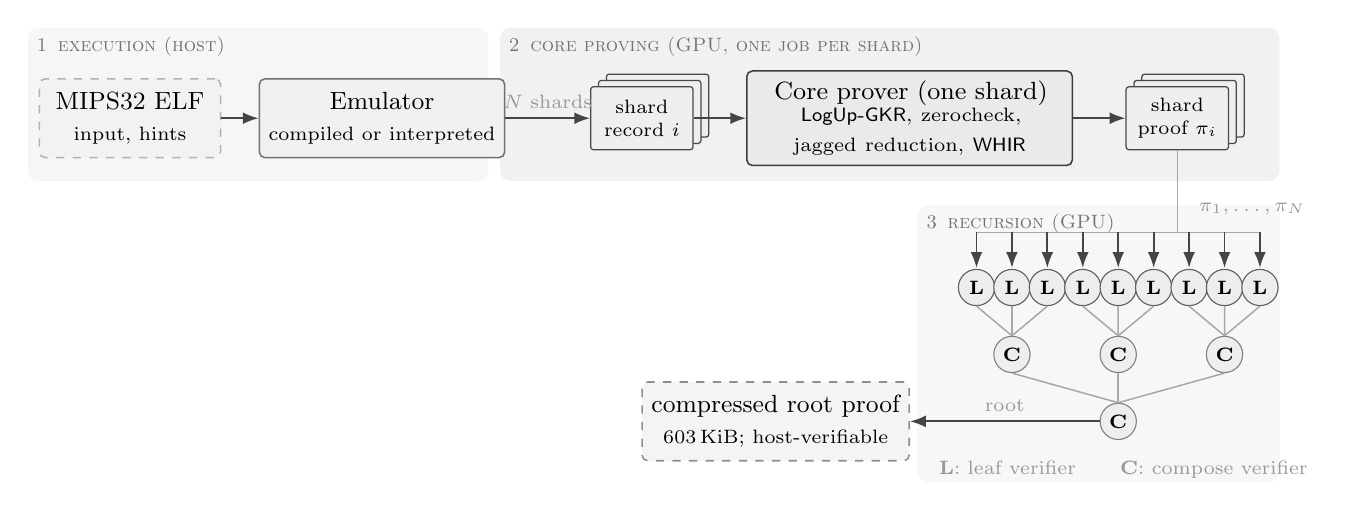
\begin{tikzpicture}[
  font=\small,
  box/.style={rectangle, draw=zirenslate!85, rounded corners=2pt, minimum height=1.0cm, align=center, fill=white, line width=0.55pt},
  host/.style={box, fill=zirenblue!8, draw=zirenblue!80},
  gpu/.style={box, fill=zirenorange!9, draw=zirenorange!85},
  io/.style={box, fill=zirenlight, dashed, draw=zirenslate!75},
  card/.style={rectangle, rounded corners=1pt, draw=zirenorange!80, fill=zirenorange!7, minimum width=1.3cm, minimum height=0.8cm, align=center, font=\scriptsize, line width=0.45pt},
  leaf/.style={circle, draw=zirenblue!90, fill=zirenblue!10, minimum size=0.46cm, inner sep=0pt, font=\scriptsize\bfseries},
  compose/.style={circle, draw=zirenteal!90, fill=zirenteal!12, minimum size=0.46cm, inner sep=0pt, font=\scriptsize\bfseries},
  a/.style={-{Latex[length=2mm]}, line width=0.65pt, zirenblue!90!black},
  ln/.style={zirenslate!85, line width=0.55pt},
  lab/.style={font=\scriptsize, zirenslate},
  bandlab/.style={font=\scriptsize\scshape, black!55, anchor=north west, inner sep=3pt},
]
% ---------------- row 1: execution and core proving (left to right)
\node[io, minimum width=2.3cm] (elf) at (0,0) {MIPS32 ELF\\{\scriptsize input, hints}};
\node[host, minimum width=2.4cm] (exec) at (3.2,0) {Emulator\\{\scriptsize compiled or interpreted}};
\node[card] at (6.7,0.16) {}; \node[card] at (6.6,0.08) {};
\node[card] (rec) at (6.5,0) {shard\\record $i$};
\node[gpu, text width=3.9cm, minimum height=1.2cm] (core) at (9.9,0) {Core prover (one shard)\\{\scriptsize \LogUp{}, zerocheck,\\jagged reduction, \WHIR{}}};
\node[card] at (13.5,0.16) {}; \node[card] at (13.4,0.08) {};
\node[card] (prf) at (13.3,0) {shard\\proof $\pi_i$};
\draw[a] (elf) -- (exec);
\draw[a] (exec) -- node[lab, above] {$N$ shards} (rec);
\draw[a] (rec) -- (core);
\draw[a] (core) -- (prf);
% ---------------- fan-in of shard proofs to the leaves
\draw[ln] (prf.south) -- (13.3,-1.45);
\draw[ln] (10.75,-1.45) -- (14.35,-1.45);
\foreach \k in {0,...,8} {
  \pgfmathsetmacro{\x}{10.75+0.45*\k}
  \draw[a] (\x,-1.45) -- (\x,-1.9);
  \node[leaf] (l\k) at (\x,-2.15) {L};
}
\node[lab, anchor=west] at (13.45,-1.15) {$\pi_1,\dots,\pi_N$};
% ---------------- recursion tree (arity <= 3)
\node[compose] (c0) at (11.2,-3.0) {C};
\node[compose] (c1) at (12.55,-3.0) {C};
\node[compose] (c2) at (13.9,-3.0) {C};
\node[compose] (root) at (12.55,-3.85) {C};
\foreach \k in {0,...,2} { \draw[ln] (l\k.south) -- (c0.north); }
\foreach \k in {3,...,5} { \draw[ln] (l\k.south) -- (c1.north); }
\foreach \k in {6,...,8} { \draw[ln] (l\k.south) -- (c2.north); }
\draw[ln] (c0.south) -- (root.north);
\draw[ln] (c1.south) -- (root.north);
\draw[ln] (c2.south) -- (root.north);
% ---------------- output: the compressed proof
\node[io, minimum width=2.8cm, fill=zirenteal!8, draw=zirenteal!80] (final) at (8.2,-3.85) {compressed root proof\\{\scriptsize 603\,KiB; host-verifiable}};
\draw[a] (root) -- node[lab, above] {root} (final);
\node[lab, anchor=north west] at (10.15,-4.23) {\textbf{L}: leaf verifier\qquad \textbf{C}: compose verifier};
% ---------------- stage bands (background)
\begin{scope}[on background layer]
  \fill[zirenblue!5, rounded corners=4pt]   (-1.3,-0.8) rectangle (4.55,1.15);
  \fill[zirenorange!6, rounded corners=4pt] (4.7,-0.8) rectangle (14.6,1.15);
  \fill[zirenteal!6, rounded corners=4pt] (10.0,-4.62) rectangle (14.6,-1.1);
  \node[bandlab] at (-1.3,1.15) {1\enspace execution (host)};
  \node[bandlab] at (4.7,1.15) {2\enspace core proving (GPU, one job per shard)};
  \node[bandlab] at (10.0,-1.1) {3\enspace recursion (GPU)};
\end{scope}
\end{tikzpicture}
}
\caption{No stage of the pipeline sees the whole run: the proof of a block of any length is assembled from fixed-size pieces. The emulator cuts the run into $N$ shards of a few million cycles and emits one record per shard; each record is proved independently as one Jagged-\WHIR{} shard proof $\pi_i$; leaf programs (L) verify one shard proof each and a range tree of compose programs (C, arity at most three) merges them; the root of the tree is the \emph{compressed proof}, the object measured throughout this paper.}
\label{fig:pipeline}
\end{figure}


The four ideas that carry the design answer those four difficulties in the same order, and are developed in the sections named. The \emph{instruction frame} (\S\ref{sec:air-frame}) removes the central control table this system's first generation used. Each opcode unit fetches its own instruction, performs accesses at fixed sub-cycle positions and passes the machine state on a bus, so a cycle costs one row of one unit. \emph{One lookup and one zerocheck} per shard (\S\ref{sec:air-logup}, \S\ref{sec:air-zerocheck}) discharge every bus and polynomial identity, batched across units and sharing one opening per column. \emph{Stacking and the jagged reduction} (\S\ref{sec:pcs}) preserve separate roots for preprocessed and main data while reducing tens of thousands of columns to one logical multilinear evaluation and one batched opening. The verifier depends only on the committed-area class and fixed column geometry. Finally, \emph{unit determinism} (\S\ref{sec:verification-det}) is the local property used by the conditional trace-uniqueness argument: two satisfying rows that agree on bus inputs must agree on bus outputs.

\subsection{Scope and limitations}
\label{sec:scope}

The proofs are not zero-knowledge. The soundness statement rests on a computational assumption for the cross-shard digest in addition to the information-theoretic bounds of the proximity test. The checked-in soundcalc report describes a schedule with 16 bits of lookup grinding, whereas the performance baseline uses none; Section~\ref{sec:iopp-soundness} therefore does not assign the measured baseline that report's numerical level. The determinism theorems cover the core machine and not the recursion machine, a substantial fraction remain open under the automation's budget, and Theorem~\ref{thm:unique} is stated rather than machine-checked. The evaluation uses one workload class on one GPU model and predates the Poseidon2 round correction. The verifying-key allowlist is enumerated from the machine's declared chip-set clusters, which are curated from the workloads it is built for rather than exhaustive over chip sets, so a guest that produces a shard outside them is refused rather than admitted (\S\ref{sec:recursion}). Timing closure and power have no counterpart in this setting, and area is measured in trace cells rather than gates.

\subsection{Related work}
\label{sec:related}

Table~\ref{tab:related} places the systems discussed along the axes of this introduction: guest instruction set, field, arithmetisation, lookup argument, commitment with its proximity test, and the regime in which each project states its soundness level.

\begin{table}[t]
\centering
\scriptsize\setlength{\tabcolsep}{3pt}
\caption{Design axes of \Ziren{} and four systems it is most often read against, from their public descriptions, read at the release named in the last column and retrieved on 2026-09-24. AIR is an algebraic intermediate representation, PCS a polynomial commitment scheme and IOPP an interactive oracle proof of proximity. The \emph{Regime} column names the basis on which each project states its soundness level; regimes and conjectures differ and levels are not comparable without the accounting of Section~\ref{sec:iopp-soundness}. These projects move quickly, so every row is a dated snapshot rather than a standing description.}
\label{tab:related}
\begin{tabular}{@{}>{\raggedright\arraybackslash}p{0.125\textwidth}
                  >{\raggedright\arraybackslash}p{0.095\textwidth}
                  >{\raggedright\arraybackslash}p{0.090\textwidth}
                  >{\raggedright\arraybackslash}p{0.105\textwidth}
                  >{\raggedright\arraybackslash}p{0.085\textwidth}
                  >{\raggedright\arraybackslash}p{0.120\textwidth}
                  >{\raggedright\arraybackslash}p{0.135\textwidth}
                  >{\raggedright\arraybackslash}p{0.075\textwidth}@{}}
\toprule
System & ISA & Field & Instruction tables & Lookup & Commitment / IOPP & Regime & Release \\
\midrule
\Ziren{} & MIPS32 & KoalaBear ($2^{31}$) & unit per opcode, frames & \LogUp{} & Jagged over \WHIR{} & unique decoding, union bound & this paper \\
SP1 Hypercube~\citep{sp1-hypercube} & RV64IM & KoalaBear & chip per opcode & \LogUp{} & Jagged over BaseFold & unique decoding, no proximity-gap conjecture & v6.8.0 \\
ZisK~\citep{zisk} & RV64IMA & Goldilocks & micro-operations, PIL2 & LogUp & PIL2 (e)STARK & not stated & v1.3.0-alpha \\
OpenVM~\citep{openvm} & own ISA, RV32IM transpiler & BabyBear & modular executor chips & LogUp & SWIRL: stacked \WHIR{} & unique decoding at the leaves, list decoding above & v2.0.2 \\
Jolt~\citep{jolt} & RV64IMAC & BN254 scalar (Dory), 128-bit (Akita) & Twist and Shout, small R1CS & Twist and Shout & Dory (default), Akita (lattice) & not stated & v0.3.0-alpha \\
\bottomrule
\end{tabular}
\end{table}

\paragraph{Chip-decomposed machines.} SP1~\citep{sp1} established the template \Ziren{} follows: one unit per opcode, \LogUp{} and recursive aggregation. SP1 Hypercube~\citep{sp1-hypercube} added the jagged commitment and shard-level lookup and zerocheck shape; its just-in-time executor~\citep{sp1-jit} is the model for ours. \Ziren{} inherits that template, the septic cross-shard digest and the shadow-read device that makes register accesses cheaper than memory accesses. It differs in the guest ISA and its frame, in opening the jagged commitment with \WHIR{} rather than BaseFold, and in reporting a union bound over components rather than a single level; both systems count query soundness in the unique-decoding regime, and SP1 states that it relies on proximity-gap theorems rather than conjectures~\citep{sp1-security} (retrieved 2026-09-24). 

\paragraph{The closest layer-level neighbour.} OpenVM~\citep{openvm} likewise has no central control table; the instruction frame specialises that idea to MIPS.
\paragraph{The closest current overlap.} OpenVM's SWIRL combines stacked \WHIR{}
with \LogUp{} interaction reduction, which is the same pair of ideas as this
paper's Jagged--\WHIR{} layer. Four axes separate them at the snapshot above:
we place columns of differing heights under ordered rounds whose committed
areas, padding included, form one logical dense vector and reduce every column
claim by the jagged sumcheck; our \WHIR{} rounds fold several variables at a
time under the per-round arity and rate schedule of Section~\ref{sec:iopp};
\KB{} rather than BabyBear changes the extension degree available for
challenges and hence the fingerprinting term; and our soundness level is a
union bound over components rather than a project target, which is a different
basis and not numerically comparable. 

\paragraph{And a second.} Ceno is a second point of proximity: its
backend selects a commitment at run time, offering a jagged reduction over
BaseFold by default and \WHIR{} as an alternative, rather than the two in
composition~\citep{ceno} (repository revision \texttt{7c58fdd4}, retrieved
2026-09-24). The composition presented here therefore lies adjacent to
published work, and what is claimed is the composition, its schedule and its
recursive verifier, not either constituent. Where the axes of the table are
design axes, no cross-system performance claim follows from them, and no
same-hardware comparison against any of these systems is attempted here.
Machine-checked constraint-system correctness is an axis the table omits
deliberately: stating where other projects stand would need a dated survey of
each project's artifacts at a fixed revision, which we have not performed, so
we report our own coverage (Section~\ref{sec:verification}) and make no
comparative claim.

\paragraph{Where the prover's work is put.} Jolt~\citep{jolt} evaluates instructions by lookups rather than by per-opcode constraints, moving the dominant cost into the lookup argument and its multiplicities; since v0.2.0 it does so through the Twist and Shout arguments~\citep{twist-shout} in place of the Lasso construction~\citep{lasso} of its original design, with a small R1CS instance for instruction fetch. \Ziren{} uses lookups for byte-granular facts and for buses, and evaluates instructions by polynomial constraints. ZisK~\citep{zisk} instead lowers the RV64IMA execution to micro-operations constrained in PIL2 and commits a STARK trace. The evaluation of Section~\ref{sec:performance} measures this system against itself.

\paragraph{Systems not contrasted above.} The wider field is larger than the
table, and we name it rather than leave it implicit. RISC Zero~\citep{risc0}
proves a RISC-V machine through a control table and a FRI-based STARK with
continuations. Cairo~\citep{cairo} and Valida~\citep{valida} take the opposite
route to \Ziren{} on the ISA question, designing an instruction set for proving
instead of inheriting a hardware one. Ceno~\citep{ceno} builds non-uniform
circuits per basic block and proves them with GKR over parallel segments.
Nexus~\citep{nexus} accumulates execution by folding rather than merging shard
proofs in a tree. Airbender~\citep{airbender} targets Mersenne-31 with a
degree-two arithmetisation and DEEP-FRI, a different point on the trade-off of
Section~\ref{sec:prelim}. Cysic~\citep{cysic} pursues dedicated proving
hardware, outside the CPU--GPU scope of Section~\ref{sec:ipcore}. None is
measured here.

\paragraph{Fields, proximity and commitment.} The field, $\Poseidon{}$ permutation~\citep{poseidon2}, constraint interfaces and transforms come from Plonky3~\citep{plonky3}. Circle STARKs~\citep{circle-starks} reach smooth Mersenne-31 domains through the circle group. \KB{} instead has two-adicity 24 and uses ordinary Reed--Solomon domains, requiring the word splitting of Section~\ref{sec:prelim}; Binius~\citep{binius,fri-binius} avoids that split with binary towers. The proximity line runs from FRI~\citep{ben2018fast} through DEEP-FRI~\citep{deep-fri} and proximity-gap bounds~\citep{proximity-gaps} to BaseFold~\citep{basefold}, STIR~\citep{stir} and \WHIR{}~\citep{whir}. Ligero~\citep{ligero} and Brakedown~\citep{brakedown} are linear-time alternatives not used here. The jagged commitment is from~\citep{jagged-pcs}, with the branching-program evaluation of Holmgren and Rothblum~\citep{hr18}; our contribution at this layer is its composition with \WHIR{} and the measured schedule. The lookup uses Hab\"ock's logarithmic derivative~\citep{haboeck} in its published GKR realisation~\citep{logup-gkr}. Plookup~\citep{plookup} and cq~\citep{cq} are univariate alternatives that do not transfer directly to this multilinear many-bus workload. The memory argument descends from~\citep{blum1994}.

\paragraph{MIPS, embedded verification, and circuit verification.} Zilch's zMIPS verifies a MIPS-like instruction model and composes instruction proofs~\citep{zilch}; o1VM documents a segmented prover intended to run in MIPS and RISC-V modes~\citep{o1vm}. \Ziren{} differs by targeting the MIPS32 execution relation used by the rollup fault-proof ecosystem, by its chip-decomposed AIR and Jagged--\WHIR{} commitment, and by its recursion and verification collateral. Cannon~\citep{cannon} is a single-step MIPS interpreter for interactive fault proofs, and its suite is one of our conformance inputs; Kona~\citep{kona} is the fault-proof program of the same ecosystem. zkMIPS~\citep{zkmips} is the first-generation \Ziren{} prover. Proofs reach constrained devices today as authentication and attestation protocols~\citep{zk-iot-survey,zpie,zekra,zra}, where the statement is small and about the device; a \zkVM{} for the device's instruction set instead makes its software execution the statement and the constrained party the verifier.

Picus~\citep{picus} introduced the determinism formulation of under-constrained circuits and an SMT solver for it; Section~\ref{sec:verification-det} states the same property and discharges it in \Lean{}, because we could not run the public solver at the unit sizes of Table~\ref{tab:chips}. OpenVM's verification project extracts the AIR of its RV32IM and precompile chips and proves refinement to Lean reference specifications~\citep{openvm-fv}; its closed opcode proofs provide a stronger correctness baseline than the partial determinism coverage reported here, while targeting a different ISA and constraint system. The accounting follows the round-by-round methodology of~\citep{whir} and is computed with \texttt{soundcalc}~\citep{soundcalc}; the ethSTARK documentation~\citep{ethstark} provides another published treatment of this style of accounting.

\subsection{Organisation}

Section~\ref{sec:prelim} defines the field, the code, and the unit, bus and determinism notions the rest of the paper is stated over. Section~\ref{sec:isa} defines the execution relation, and Section~\ref{sec:ipcore} fixes what is measured and what is not. Section~\ref{sec:argument} states the argument system as a protocol over four primitives. Sections~\ref{sec:air} to~\ref{sec:iopp} instantiate them: Section~\ref{sec:air} builds the arithmetisation and proves the bus lemmas and the trace-uniqueness theorem, Section~\ref{sec:pcs} builds the jagged commitment, and Section~\ref{sec:iopp} instantiates the opening and accounts for soundness component by component. Section~\ref{sec:recursion} then composes shard proofs into a block proof and states what binds that composition to the advertised machine. Section~\ref{sec:verification} describes the verification flow and its findings, and Section~\ref{sec:performance} the concrete efficiency. Appendix~\ref{sec:executor} gives the just-in-time executor and Appendix~\ref{sec:app-ipcore} specifies the system interfaces, configuration parameters, integration paths and delivered verification artifacts.

\section{Preliminaries}
\label{sec:prelim}

\subsection{Field, polynomials and codes}

\paragraph{Field.} All traces live over the prime field $\F = \KB{}$, $p = 2^{31} - 2^{24} + 1$. Its multiplicative group has two-adicity 24, which bounds the Reed--Solomon domains available to the proximity test: the rate schedule of Section~\ref{sec:iopp} is chosen so that the largest domain stops one bit short of that limit. Random challenges and all sumcheck arithmetic use the degree-four binomial extension $\EF = \F[X]/(X^4 - 3)$; a sumcheck round polynomial of degree $d$ therefore has soundness error $d/|\EF| \approx d \cdot 2^{-124}$ per round. Note that $2^{32} > p$: a 32-bit machine word cannot be represented by a single field element, and every word in the arithmetisation is a vector of four field elements holding its little-endian bytes.

\paragraph{Multilinear extensions and sumcheck.} For $f: \{0,1\}^n \to \F$ the multilinear extension $\widetilde f \in \F[X_1,\dots,X_n]$ is the unique multilinear polynomial agreeing with $f$ on the hypercube, $\widetilde f(\bm z) = \sum_{\bm b} f(\bm b)\,\eqf(\bm b, \bm z)$ with $\eqf(\bm b, \bm z) = \prod_i (b_i z_i + (1-b_i)(1-z_i))$. The sumcheck protocol~\citep{lund1992algebraic} reduces a claim $\sum_{\bm b \in \{0,1\}^n} g(\bm b) = \sigma$ about a low-degree $g$ to a claim $g(\bm r) = \sigma'$ at a random $\bm r \in \EF^n$ in $n$ rounds, each sending a univariate polynomial of degree $\deg g$. We write a claim about a multilinear $\widetilde f$ as the pair $(\bm z, v)$ meaning $\widetilde f(\bm z) = v$.

\paragraph{Reed--Solomon and constrained Reed--Solomon codes.} For a smooth domain $L \subset \F^{*}$ (a coset of a subgroup of order $2^{\ell}$) the code $\RS[\F, L, m]$ is the set of functions $L \to \F$ that agree with a polynomial of degree $< 2^m$; its rate is $\rho = 2^m/|L|$. Identifying the coefficient vector of such a polynomial with a function on $\{0,1\}^m$, a codeword is also the evaluation of an $m$-variate multilinear $\widehat f$ at the points $(x, x^2, x^4, \dots, x^{2^{m-1}})$, $x \in L$. Following~\citep{whir}, the \emph{constrained} code $\CRS[\F, L, m, \widehat w, \sigma]$ is the subset of $\RS[\F, L, m]$ whose multilinear satisfies $\sum_{\bm b \in \{0,1\}^m} \widehat w(\widehat f(\bm b), \bm b) = \sigma$ for a weight polynomial $\widehat w$; the weight $\widehat w(Z, \bm X) = Z \cdot \eqf(\bm X, \bm z)$ expresses the evaluation claim $\widehat f(\bm z) = \sigma$. A \emph{fold} of a codeword by a challenge $\alpha$ maps $f: L \to \F$ to $\Fold(f, \alpha)(x^2) = \tfrac{f(x) + f(-x)}{2} + \alpha \tfrac{f(x) - f(-x)}{2x}$, which is a codeword of $\RS[\F, L^{(2)}, m-1]$ whenever $f$ is a codeword, and equals the partial evaluation of $\widehat f$ at $X_1 = \alpha$.

\paragraph{Hashing and transcripts.} Merkle commitments and the Fiat--Shamir transcript~\citep{fiat-shamir} use the $\Poseidon{}$ permutation~\citep{poseidon2} over $\F$ at width 16 with a 248-bit digest (eight field elements). Its S-box has degree three, so the round schedule is eight full and twenty partial rounds, the parameters tabulated for a 31-bit prime at that width and degree; the same permutation is used by the transcript, the commitment trees and the recursion machine, so a single round schedule fixes all three. Proof-of-work grinding of $b$ bits means the prover searches for a nonce whose absorption yields $b$ leading zero bits in the squeezed challenge; it multiplies the cost of the corresponding cheating strategy by $2^{b}$ and appears additively in the security accounting.

\subsection{Units, buses and determinism}
\label{sec:prelim-chips}

\begin{definition}[Unit]
\label{def:chip}
A \emph{unit} (a \emph{chip} in the implementation and in the literature this design descends from) is a table over $\F$ of a fixed width $w$ together with a set of polynomial constraints of degree at most three in the $w$ columns of one row, a distinguished boolean column $\mathsf{is\_real}$ gating every constraint, and a set of \emph{interactions}. A row is \emph{satisfying} if it satisfies every constraint.
\end{definition}

\begin{definition}[Interaction and bus]
\label{def:bus}
An interaction of a unit is a triple $(\mathsf{bus}, \bm f, m)$ where $\mathsf{bus}$ is a name, $\bm f$ is a tuple of linear expressions in the row's columns and $m$ is a linear expression in the columns (the multiplicity), marked as a \emph{send} or a \emph{receive}. Multiplicities are constrained to small non-negative integers---in the arithmetisation of Section~\ref{sec:air} they are zero, one, or a value range-checked against the byte table---so that a sum of them over the rows of a shard is far below $p$ and is read as an integer. For a set of tables, the \emph{multiset of a bus} is $\{(\bm f(r))\}$ with multiplicity $\sum m(r)$ over the sends of all rows $r$ of all units, and likewise for the receives. A bus \emph{balances} if its send and receive multisets are equal; because the multiplicities stay small, the fraction identity of Section~\ref{sec:air-logup} over $\EF$ is equivalent to this multiset equality.
\end{definition}

\paragraph{Lookups as fractions.} A lookup argument proves that two multisets of field-element tuples agree. In the logarithmic-derivative form of Hab\"ock and its GKR realisation~\citep{haboeck,logup-gkr}---written \LogUp{} throughout---each tuple $\bm f$ on bus $\mathsf{bus}$ with multiplicity $m$ contributes a fraction $m/(\alpha - \mathsf{bus} - \sum_{j \ge 1} \beta^{j} f_j)$ for random $\alpha, \beta \in \EF$, senders and receivers must sum to the same value, and the sum is computed by a layered GKR circuit~\citep{gkr-cmt} whose layers are proved by sumcheck. Section~\ref{sec:air-logup} proves all buses of a shard by one such argument.

\paragraph{Zerocheck.} A \emph{zerocheck} proves that a polynomial vanishes on a set of points: to show $g(\bm b) = 0$ for every $\bm b$ in a subcube, the verifier samples $\bm r$ and the prover runs a sumcheck on $\sum_{\bm b} \eqf(\bm b, \bm r)\, g(\bm b)$, which is zero for every $\bm r$ if and only if $g$ vanishes on the subcube, up to the sumcheck's error. Section~\ref{sec:air-zerocheck} proves all polynomial constraints of a shard by one such check.

\begin{definition}[Shard relation]
\label{def:shard}
A \emph{shard} is a set of tables, one per unit, together with public values $\mathsf{pv}$ (the entry and exit state, the address cursors of the global memory tables and the septic digest, Section~\ref{sec:isa}). It is \emph{valid} if every real row is satisfying and every bus balances, where the public-values table contributes the entry state as a send and the exit state as a receive on the state bus, and the program bus is received by the preprocessed program table with the recorded multiplicities.
\end{definition}

\begin{definition}[Inputs, outputs and determinism of a unit]
\label{def:det}
For a unit $U$, the \emph{inputs} $I_U(r)$ of a row $r$ are the values the row consumes from elsewhere: the tuples of its receives, the program tuple it fetches, and the previous-value part of its memory accesses. The \emph{outputs} $O_U(r)$ are the values it produces for elsewhere: the tuples of its sends other than the fetch, and the new-value part of its memory accesses. Fetch and previous value are sends in the sense of Definition~\ref{def:bus}---the preprocessed table and the earlier access are their sources---but they are inputs of the row, and the direction of a bus interaction is therefore not by itself the direction of the data. $U$ is \emph{deterministic} if for all satisfying real rows $r, r'$,
\[
  I_U(r) = I_U(r') \;\Rightarrow\; O_U(r) = O_U(r').
\]
This is the notion of Picus~\citep{picus} adapted to the interaction language: whatever a row consumes from another table is an input, whatever it produces for another table is an output.
\end{definition}

\paragraph{Cost metrics.} Throughout, the \emph{trace area} of a shard or a block is the sum over units of rows $\times$ columns of the committed main trace, in cells; the \emph{(row, interaction) count} is the number of bus interactions summed over all rows, which is the number of leaves of the lookup circuit; and \emph{throughput} is the number of proved guest cycles per second of wall-clock time. Section~\ref{sec:performance} relates the three to measured prover time.

\section{The machine and its execution relation}
\label{sec:isa}

\subsection{MIPS32 as a guest}

Throughout this paper MIPS32 means Release 2 of the specification, the revision this work targets and the last before Release~6 re-encoded the instruction set incompatibly. The guest machine is a 32-bit MIPS32 core with 32 integer registers (register 0 hard-wired to zero), the \texttt{HI}/\texttt{LO} pair written by multiplication and division, and a little-endian byte-addressed memory. Three features of the ISA shape the arithmetisation more than anything else.

\paragraph{Branch-delay slots.} The instruction that follows a branch or jump is executed before control transfers. The machine state therefore carries a program counter \emph{pair}: the address of the current instruction and the address of the one that follows it. A sequential instruction advances the pair as $(\mathsf{pc}, \mathsf{next\_pc}) \mapsto (\mathsf{next\_pc}, \mathsf{next\_pc} + 4)$; a branch instruction sets $\mathsf{next\_next\_pc}$ to the target or to $\mathsf{next\_pc}+4$. Consequently the successor of a sequential instruction is \emph{data}, not $\mathsf{pc}+4$: when the instruction sits in a delay slot its successor is the branch target. Every instruction row carries $\mathsf{next\_pc}$ as a witnessed column for this reason.

\paragraph{Unaligned and narrow accesses.} \texttt{LB}, \texttt{LBU}, \texttt{LH}, \texttt{LHU}, \texttt{SB}, \texttt{SH} address individual bytes and half-words of a word, and \texttt{LWL}/\texttt{LWR}/\texttt{SWL}/\texttt{SWR} merge the left or right part of an unaligned word with a register. Memory is modelled at word granularity, so these instructions select and merge bytes of a word in-circuit; they get chips of their own (Section~\ref{sec:air-chips}).

\paragraph{Bit manipulation.} \texttt{EXT}, \texttt{INS}, \texttt{WSBH}, \texttt{SEB}/\texttt{SEH}, \texttt{ROTR}, \texttt{CLO}/\texttt{CLZ} and the conditional moves are common in hashing and serialisation code. All of them are supported natively rather than lowered.

\subsection{Syscalls and precompiles}

Guest programs reach the host through \texttt{SYSCALL}. Besides input/output the syscall table exposes \emph{precompiles}: SHA-256, Keccak-f[1600], the $\Poseidon{}$ permutation, curve arithmetic on secp256k1, secp256r1, BN254, BLS12-381 and Ed25519, field arithmetic for BN254 and BLS12-381, 256-bit modular and $256\times 2048$-bit multiplication. A precompile reads and writes guest memory directly; each invocation becomes one or more rows of a dedicated chip whose memory accesses are timestamped at the invoking cycle.

\paragraph{Hash functions.} Hashing is the dominant primitive of the workloads this class of machine is asked to prove, and it motivates the accelerator interface. An unaccelerated guest computing SHA-256 or Keccak in MIPS instructions pays tens of instructions per round, each occupying an instruction-chip row, whereas an accelerator computes a permutation in a handful of wide rows. Three hash families are accelerated. SHA-256 is split into its message-schedule extension and compression rounds, with a control chip sequencing memory accesses. Keccak-f[1600] is a sponge chip with its own controller and, at 2\,637 columns, is one of the two widest chips (Table~\ref{tab:chips}). $\Poseidon{}$ is accelerated for guests that verify proofs of this system. The same permutation also implements Merkle commitments and the Fiat--Shamir transcript (Section~\ref{sec:prelim}) and appears in the recursion machine (Section~\ref{sec:recursion}). Hint data written by the host into untouched memory becomes part of the memory's initial state (Section~\ref{sec:air-memory}), so it remains subject to the argument's range discipline.

\subsection{Clock, shards and the execution record}

Execution is divided into \emph{shards}. Within a shard a clock $\mathsf{clk}$ advances by five per instruction; a syscall additionally advances it by a bounded number of ticks so that the memory accesses of a precompile fit strictly between the calling instruction and its successor. An instruction executes at $\mathsf{clk}$ and its memory and register accesses occupy the four \emph{sub-cycle positions} $\mathsf{clk}+1,\dots,\mathsf{clk}+4$, one per operand role (Section~\ref{sec:air-frame}), so a $(\mathsf{shard}, \mathsf{clk} + \mathsf{pos})$ pair identifies every access uniquely and the memory argument timestamps an access by $\mathsf{clk}+\mathsf{pos}$. The clock is bounded by $2^{25}$, which caps a shard at $2^{25}/5 \approx 6.71$\,M cycles whatever the configured shard size says. The clock is witnessed as a 16-bit limb and a 10-bit high limb, the same decomposition the memory argument range-checks. A shard therefore closes on whichever of three bounds binds first: that fence; the configured shard size, a few million cycles, against which the executor compares $\mathsf{clk} + \mathsf{max\_syscall\_cycles}$ after scaling the configured figure by four, since it is given in cycles and the clock advances by five per instruction; or a chip's height budget. Which one binds depends on the configuration, and Section~\ref{sec:performance} reports the shard counts that result from four of them.

At a shard boundary the emulator emits, for every memory word touched in the shard, the value and timestamp of its first and last access; these are the leaves of the cross-shard memory argument. The prover arithmetises a shard record containing per-chip event lists, the touched-address ledger and public values. Those public values contain the committed-output and deferred-proof digests, entry and exit program-counter pairs and clocks, exit code, shard indices, global-memory cursors and row counts, and the septic digest of Section~\ref{sec:air-global}. They are the interface through which consecutive shards and recursion layers are chained.

\subsection{The execution relation}
\label{sec:isa-emulator}

Write $\mathsf{Emulate}(P, \mathsf{in}, \mathsf{hint}) = (\mathsf{out}, e)$ for the relation this section defines: the machine of \S\ref{sec:isa} started on the program image $P$ with the two streams available to it, run until it halts, produces the output stream $\mathsf{out}$ and the exit status $e$. It is deterministic: no step reads a clock, a random source or any host state other than the streams.

The relation is realised twice, and the two realisations must agree. The reference is an interpreter: it implements every instruction, every syscall and every error path, and it is the only one that emits the event record the prover consumes. A just-in-time compiler serves the two jobs that dominate wall-clock time and need no events, namely running a guest for its output alone and producing, per shard, the descriptor from which a worker replays that shard. Three checks connect them, none of which is a proof of equivalence for every program: the descriptors of a compiled run are byte-identical to an interpreted one on the tested corpus, the specification vectors of Section~\ref{sec:verification} run on both, and continuous integration compares digests of the emitted records. The difference that matters to the rest of the paper is rate, because a host feeding several accelerators is bound by the executor rather than by the accelerator (\S\ref{sec:perf-host}); Appendix~\ref{sec:executor} gives the mechanism.

\section{What is implemented, and what is measured}
\label{sec:ipcore}

The sections that follow describe the proof system from the inside. This section identifies the implemented system boundary, because that boundary determines what can be measured and what those measurements mean. The processor is represented by arithmetic constraints rather than by synthesisable RTL, and what is evaluated here is the proving and verification software stack running on CPUs and GPUs.

\paragraph{Four configurations, and which claim attaches to which.} One
warning belongs here rather than distributed through the sections that make
the claims. No single revision of this system exhibits every property reported
in this paper, and the paper does not pretend otherwise. The commit named on
the title page is the one the construction is described from, and it carries
the corrected $\Poseidon{}$ round schedule. The timings and proof sizes of
Section~\ref{sec:performance} were taken on earlier revisions of the same
branch, before that correction and with the lookup grinding set to zero. The
soundness figures of \S\ref{sec:iopp-soundness} are for the checked-in
configuration, which spends 16 bits on that grinding and which
Section~\ref{sec:performance} therefore does not measure. And the determinism
count of \S\ref{sec:verification-det} is for the constraint system with the
syscall-bus change of \S\ref{sec:verification-findings} applied, which two
chips separate from the system that was timed. Each section states its own
configuration where it reports; the reason to say it once here is that a
reader who takes a number from one section and a number from another is
comparing revisions, not configurations of one revision.

\Ziren{} has three implementation layers. The execution layer runs a MIPS32 program and emits the witness record. The proof layer constrains, commits and recursively compresses that record. The deployment layer schedules the work on host processors and GPUs and exposes standalone and wrapped verifiers. Table~\ref{tab:design-correspondence} maps these layers to the quantities evaluated in this paper and prevents proof-system metrics from being conflated with silicon metrics.

\begin{table}[t]
\centering
\small
\caption{Implemented verifiable-system components and their evaluated quantities. None of the reported quantities is a silicon PPA metric.}
\label{tab:design-correspondence}
\begin{tabular}{>{\raggedright\arraybackslash}p{0.23\textwidth} >{\raggedright\arraybackslash}p{0.42\textwidth} >{\raggedright\arraybackslash}p{0.25\textwidth}}
\toprule
System component & Implementation & Reported quantity \\
\midrule
Guest execution & interpreter or JIT executor for MIPS32 & guest cycles and execution rate \\
Execution relation & opcode-specific trace tables, identities and multiset buses & rows, columns, interactions and trace cells \\
Proof generation & lookup, zerocheck, Jagged--\WHIR{} opening and recursion & proof bytes and soundness terms \\
Verification & standalone compressed-proof verifier or optional outer wrapper & acceptance result and verified public values \\
Deployment runtime & coordinator plus one or more GPU proving workers & wall-clock time and proved guest cycles/s \\
\bottomrule
\end{tabular}
\end{table}

\paragraph{Trace area belongs to the proof relation.}\label{sec:ipcore-platform} The trace area of a chip is its column count times its row count, and both are fixed by the constraint system and the execution rather than by the machine that runs the prover. Trace area determines how many field elements the prover must commit and open, and therefore contributes to proof cost. It is not measured in square millimetres and does not convert into die area. An arithmetisation change can nevertheless be stated once, in cells, and evaluated on different accelerators, which is why the per-chip census of Section~\ref{sec:performance} is given in cells before it is given in seconds.

\paragraph{Throughput belongs to the implementation--accelerator pair.} Proved guest cycles per second is not a property of the execution relation alone. It is what one implementation achieves on a specified accelerator, and a different device, or more of them, changes the figure without altering a constraint. Three things follow. Scaling has to be reported across device counts rather than as a single number. Figures measured on other projects' hardware are context, not comparison. And the transferable part of the performance analysis is the cost model, which predicts prover work from area and interaction count while the implementation and accelerator determine the constants.

\paragraph{Realisation boundary.} This paper evaluates a software proof system deployed on a host processor with one to four GPUs. It reports no RTL synthesis, place-and-route, process node, timing closure, silicon area or energy measurement; every frequency figure is proved guest cycles per second and is not a hardware clock. Section~\ref{sec:verification} reports how the executor, constraint system and recursive verifier are checked, together with the coverage that remains incomplete. Consequently, the results support claims about an implemented verifiable-computation system, its proof cost and heterogeneous-system throughput, but not claims about a fabricated processor or FPGA implementation.

Appendix~\ref{sec:app-ipcore} collects the reference material a deployer needs: interfaces, variable parameters, integration modes and delivered verification artifacts.

\section{The argument system}
\label{sec:argument}

This section states what is proved and how, independently of how any component
is built. A \emph{shard argument} reduces every claim about one shard's
execution to a single evaluation of a single committed polynomial, and one
opening authenticates it. A \emph{block argument} composes shard arguments by
recursion into one proof of the relation $\mathcal R$ of
Section~\ref{sec:statement}. Sections~\ref{sec:air} to~\ref{sec:recursion}
instantiate each component named here, and Section~\ref{sec:verification} asks
whether the instantiation admits only executions of the advertised machine.

\subsection{Parameters}
\label{sec:argument-params}

The protocol is stated over the following parameters, and is symbolic in all of
them: a different choice gives a different instantiation of the same protocol.
Numeric values are fixed where the component is built.
Table~\ref{tab:whir-schedule} fixes the proximity-test schedule of the
checked-in core and compress profiles, \S\ref{sec:pcs-geometry} the stacking
height and the row cube, \S\ref{sec:prelim} the permutation schedule,
\S\ref{sec:isa} the clock fence and \S\ref{sec:recursion} the recursion
arity. The measured baseline of Section~\ref{sec:performance} differs from the
checked-in configuration in two of these parameters, and one of them is a
security parameter: it sets the lookup grinding to zero, and it carries the
degree-seven $\Poseidon{}$ round count rather than the corrected degree-three
schedule (\S\ref{sec:prelim}).

\begin{itemize}
  \item The base field $\F$ and the extension $\EF$ from which challenges are
  drawn. The extension degree bounds every soundness term of the form
  $\deg/|\EF|$.
  \item The permutation used for the transcript and for the commitment trees,
  with its round counts, and the arity of those trees.
  \item The stacking height $H=2^{\ell}$, the row cube $2^{n}$, and the bucket
  rule that maps a round's real area to its committed area
  (\S\ref{sec:pcs-geometry}). These fix the committed geometry, and with it
  the set of recursion programs a prover can produce.
  \item For the proximity test: the initial rate $\rho$, the per-round folding
  factors, the query counts, the number of out-of-domain samples, the grinding
  bits spent on each query phase and on the bus challenges, and the regime in
  which the query soundness is counted.
  \item For recursion: the arity of a compose node and the height of the tree of
  admissible recursion keys (\S\ref{sec:recursion}).
  \item For the machine: the configured shard size, the clock fence and the
  per-unit height budgets, whichever of which binds first closing a shard
  (\S\ref{sec:isa}).
  \item The guest-accelerator set, which fixes the precompile units a shard may
  contain and therefore the unit set itself (\S\ref{sec:ipcore-config}).
  \item For the cross-shard digest: the curve and its extension, the bound
  $N_{\mathrm{int}}$ on the interactions a block proof may contain, and the
  per-interaction multiplicity bound $B$ (\S\ref{sec:air-digest-security}).
\end{itemize}

Two properties of the instantiation are worth stating with the parameters
rather than leaving to a discussion. Query soundness is counted in the
unique-decoding regime, where no conjecture is needed, rather than at the
Johnson bound or towards capacity (\S\ref{sec:iopp-soundness}). And no
blinding is applied anywhere: the protocol is succinct, not hiding, and a proof
reveals what its committed trace reveals.

\subsection{Syntax and components}
\label{sec:argument-components}

We state the shard argument and each primitive it uses as a tuple of
algorithms, so that the protocol of \S\ref{sec:argument-shard} can be read
against interfaces rather than against any one construction. Throughout,
$\mathsf{pp}$ are the public parameters of \S\ref{sec:argument-params} and
$\tau$ is the transcript the Fiat--Shamir transform maintains.

A \emph{shard argument} is a tuple $\mathsf{SA} = (\mathsf{Setup},
\mathsf{Prove}, \mathsf{Verify})$:

\begin{description}
  \item[$\mathsf{Setup}(\mathsf{pp}, P) \to (\mathsf{pk}, \mathsf{vk})$:] on
  input a program image $P$, commits to the program ROM and the preprocessed
  tables and outputs a proving key and a verifying key.
  \item[$\mathsf{Prove}(\mathsf{pk}, T) \to \pi$:] on input the execution
  record $T$ of one shard, outputs a shard proof.
  \item[$\mathsf{Verify}(\mathsf{vk}, \mathsf{pv}, \pi) \to b$:] on input the
  shard's public values, outputs $b \in \{0,1\}$.
\end{description}

It is built from four primitives. A \emph{unit} is a table of columns over
$\F$ with a constraint system and a set of bus interactions
(Definitions~\ref{def:chip} and~\ref{def:bus}), and a shard is a set of units
with a shared public-value row; units are data rather than algorithms, so they
carry no syntax here. The other three do.

A \emph{bus argument} $\mathsf{BA} = (\mathsf{Prove}, \mathsf{Verify})$
certifies that the multiset of tuples sent on each bus equals the multiset
received:

\begin{description}
  \item[$\mathsf{BA.Prove}(\tau, \{U_i\}) \to (\pi_{\mathrm{bus}}, \bm z, \{v_{i,j}\})$:]
  outputs a proof together with the point $\bm z$ and the claimed evaluations
  $v_{i,j}$ of column $j$ of unit $i$ at $\bm z$.
  \item[$\mathsf{BA.Verify}(\tau, \pi_{\mathrm{bus}}) \to (\bm z, \{v_{i,j}\}) \lor \bot$:]
  accepts and outputs the point and the claims it has reduced to, or rejects.
\end{description}

A \emph{constraint argument} $\mathsf{CA} = (\mathsf{Prove}, \mathsf{Verify})$
has the same shape and certifies instead that every unit's constraints vanish
on its real rows, reducing that claim to evaluations at the same point.

A \emph{jagged commitment} $\mathsf{JC} = (\mathsf{Commit}, \mathsf{Reduce},
\mathsf{Open}, \mathsf{VerifyOpen})$ carries columns of differing heights:

\begin{description}
  \item[$\mathsf{JC.Commit}(\mathsf{pp}, (c_1,\dots,c_M)) \to (\mathsf{com}, \mathsf{st})$:]
  on input $M$ columns of arbitrary heights, places them into the committed
  geometry and outputs a commitment and prover state.
  \item[$\mathsf{JC.Reduce}(\mathsf{st}, \{(i, \bm z, v_i)\}) \to (\pi_{\mathrm{jag}}, \bm z^{*}, v^{*})$:]
  reduces any set of column-evaluation claims to a single evaluation
  $v^{*}$ of one dense multilinear polynomial at one point $\bm z^{*}$.
  \item[$\mathsf{JC.Open}(\mathsf{st}, \bm z^{*}) \to \pi_{\mathrm{open}}$] and
  \item[$\mathsf{JC.VerifyOpen}(\mathsf{com}, \bm z^{*}, v^{*}, \pi_{\mathrm{open}}) \to b$:]
  authenticate that single evaluation against the commitment.
\end{description}

Only the last interface constrains the others: because every claim is reduced
to one evaluation of one polynomial, the number of units, their widths and
their heights are invisible to the opening, and a unit may be added, widened or
removed without changing the layer above it.

\subsection{The shard argument}
\label{sec:argument-shard}

Protocol~\ref{prot:shard} states the reduction.
Each step ends with claims of the same kind it began with, evaluations of
committed columns, so the steps compose without the verifier ever reading a
column.

\begin{protocol}[Shard argument]
\label{prot:shard}
\textbf{Statement:} a verifying key committing to the program and the
preprocessed tables, and the public values of one shard.\\
\textbf{Witness:} the shard's execution record.
\begin{enumerate}
  \item \textbf{Commit.} The prover arranges each unit's events into rows,
  places the columns of each commitment round into one dense vector and
  commits to it. Round order is fixed and the per-unit dimensions enter the
  transcript, so the geometry is public before any challenge is drawn
  (Section~\ref{sec:pcs}).
  \item \textbf{Buses.} The verifier draws the bus challenges. The prover runs
  the bus argument, which reduces every send and receive of every unit to
  column evaluations at one point (Section~\ref{sec:air-logup}).
  \item \textbf{Constraints.} The verifier draws the constraint challenges. The
  prover runs the constraint argument on the same point, so each column is
  opened once for both arguments (Section~\ref{sec:air-zerocheck}).
  \item \textbf{Jagged reduction.} The column claims of the two previous steps,
  together with explicit zero claims for the gaps in the committed geometry,
  are batched and reduced to one evaluation of the dense polynomial
  (Section~\ref{sec:pcs-jagged}).
  \item \textbf{Assist.} The verifier does not materialise the weight table the
  previous step reduced against. A second sumcheck over the public column
  boundaries certifies it, and any point-extension coordinates are sampled
  here, in an order that is itself part of the protocol
  (Section~\ref{sec:pcs-jagged-assist}).
  \item \textbf{Opening.} One batched opening authenticates that evaluation
  against every commitment of step~1 (Section~\ref{sec:iopp}).
\end{enumerate}
\textbf{Output:} a shard proof whose public values carry the entry and exit
machine state, the memory-address cursors, the digest of committed output and
the exit code that the relation of Section~\ref{sec:statement} is stated over,
and a digest of the interactions this shard leaves unbalanced.
\end{protocol}

\paragraph{From shards to a block.} A shard argument proves one shard in
isolation. Three things tie the shards of one execution together, and each is
discharged where it arises rather than by the opening: the machine state
chains through the public values, the memory-address cursors tile, and the
interactions that cross a shard boundary accumulate into a digest that must
cancel over the whole execution (Section~\ref{sec:air-global}). A recursion
layer then verifies shard proofs inside the argument system itself and merges
them, so that the verifier of a block reads one proof rather than one per
shard (Section~\ref{sec:recursion}).

\paragraph{What is proved.} Two statements carry the construction, and both are
conditional in ways the paper makes explicit rather than hiding.
Theorem~\ref{thm:composition} bounds a cheating prover for the whole tree by
the number of random-oracle queries times the sum of the per-node errors, plus
the digest term, under a per-node round-by-round premise and a hypothesis about
composed extractors. Theorem~\ref{thm:unique} shows that two satisfying traces for the same
program and public values agree up to permutation, given unit determinism and
the real-row premises that Section~\ref{sec:verification} reports coverage
for; identifying that trace with an execution of the machine needs the
conformance evidence of the same section.
Neither statement is about a particular unit set, a particular field or a
particular proximity test; those are the instantiation, fixed where each
component is built.

\section{The arithmetisation}
\label{sec:air}

Figure~\ref{fig:processor} shows instruction chips connected by buses to a program ROM, memory subsystem and lookup tables. For a chip in the sense of Definition~\ref{def:chip}, the column count is its datapath width and the row count is its activity for an execution. A \emph{bus} is an interconnect on which chips exchange tuples. The lookup argument of Section~\ref{sec:air-logup} acts as the wiring by proving that every tuple driven on a bus is consumed exactly once. The area of the design is the sum over chips of rows $\times$ columns (\emph{trace cells}); Section~\ref{sec:performance} reports it per chip, as a gate-count report would.

\begin{figure}[t]
\centering
\resizebox{\textwidth}{!}{% Ziren as a processor block diagram: units (chips) and buses (interactions).
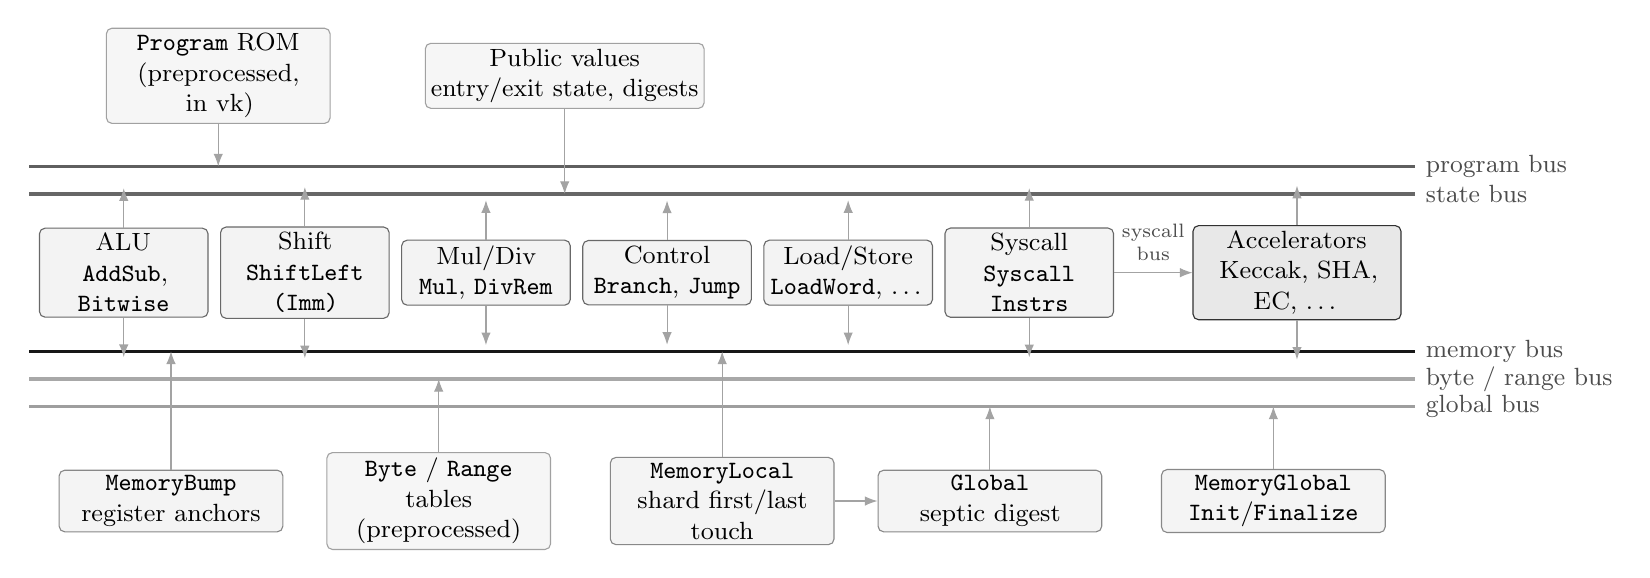
\begin{tikzpicture}[
  every node/.style={font=\small},
  unit/.style={rectangle, draw=zirenblue!85, rounded corners=2pt, text width=2.0cm, minimum height=0.7cm, align=center, fill=zirenblue!7, inner sep=2pt},
  accel/.style={unit, draw=zirenorange!90, fill=zirenorange!10},
  mem/.style={rectangle, rounded corners=2pt, draw=zirenteal!85, text width=2.7cm, minimum height=0.7cm, align=center, fill=zirenteal!8, inner sep=2pt},
  rom/.style={rectangle, rounded corners=2pt, draw=zirengold!90!black, text width=2.7cm, minimum height=0.7cm, align=center, fill=zirengold!12, inner sep=2pt},
  bus/.style={line width=1.15pt, zirenslate!85},
  programbus/.style={bus, zirenblue!90},
  statebus/.style={bus, zirenteal!90!black},
  memorybus/.style={bus, zirenorange!90!black},
  globalbus/.style={bus, zirenslate!95},
  buslab/.style={font=\small, black!70, right},
  tap/.style={-{Latex[length=1.6mm]}, thin, zirenslate!90},
]
  % instruction units (functional units), pitch 2.3 cm
  \node[unit] (alu)   at (0,0)    {ALU\\\texttt{AddSub}, \texttt{Bitwise}};
  \node[unit] (shift) at (2.3,0)  {Shift\\\texttt{ShiftLeft}\\\texttt{(Imm)}};
  \node[unit] (mul)   at (4.6,0)  {Mul/Div\\\texttt{Mul}, \texttt{DivRem}};
  \node[unit] (ctl)   at (6.9,0)  {Control\\\texttt{Branch}, \texttt{Jump}};
  \node[unit] (ld)    at (9.2,0)  {Load/Store\\\texttt{LoadWord}, \ldots};
  \node[unit] (sys)   at (11.5,0) {Syscall\\\texttt{Syscall}\\\texttt{Instrs}};
  \node[accel, text width=2.5cm] (pre) at (14.9,0) {Accelerators\\Keccak, SHA, EC, \ldots};

  % buses
  \draw[programbus] (-1.2,1.35) -- (16.4,1.35) node[buslab] {program bus};
  \draw[statebus] (-1.2,1.0)  -- (16.4,1.0)  node[buslab] {state bus};
  \draw[memorybus] (-1.2,-1.0) -- (16.4,-1.0) node[buslab] {memory bus};
  \draw[bus] (-1.2,-1.35) -- (16.4,-1.35) node[buslab] {byte / range bus};
  \draw[globalbus] (-1.2,-1.7) -- (16.4,-1.7) node[buslab] {global bus};
  \foreach \u in {alu,shift,mul,ctl,ld,sys,pre} {
    \draw[tap] (\u.north) -- ++(0,0.5);
    \draw[tap] (\u.south) -- ++(0,-0.5);
  }
  \draw[tap] (sys.east) -- node[above=1pt, font=\scriptsize, black!70, align=center] {syscall\\bus} (pre.west);

  % tables and memory units
  \node[rom] (prog) at (1.2,2.5)  {\texttt{Program} ROM\\(preprocessed, in vk)};
  \node[rom, text width=3.4cm] (pv)   at (5.6,2.5)  {Public values\\entry/exit state, digests};
  \node[mem] (bump) at (0.6,-2.9)  {\texttt{MemoryBump}\\register anchors};
  \node[rom] (byte) at (4.0,-2.9)  {\texttt{Byte} / \texttt{Range} tables\\(preprocessed)};
  \node[mem] (loc)  at (7.6,-2.9)  {\texttt{MemoryLocal}\\shard first/last touch};
  \node[mem] (glob) at (11.0,-2.9) {\texttt{Global}\\septic digest};
  \node[mem] (init) at (14.6,-2.9) {\texttt{MemoryGlobal}\\\texttt{Init}/\texttt{Finalize}};

  \draw[tap] (prog.south) -- (1.2,1.35);
  \draw[tap] (pv.south) -- (5.6,1.0);
  \draw[tap] (bump.north) -- (0.6,-1.0);
  \draw[tap] (byte.north) -- (4.0,-1.35);
  \draw[tap] (loc.north) -- (7.6,-1.0);
  \draw[tap] (loc.east) -- (glob.west);
  \draw[tap] (glob.north) -- (11.0,-1.7);
  \draw[tap] (init.north) -- (14.6,-1.7);
\end{tikzpicture}
}
\caption{Each executed instruction occupies one opcode-chip row, and every relation between chips crosses a named bus. The program and lookup tables are preprocessed; public values close the state chain and carry the cross-shard digests.}
\label{fig:processor}
\end{figure}

This section defines the constrained execution relation within the system boundary of Section~\ref{sec:ipcore}. The chip widths determine its per-chip trace area (Appendix~\ref{sec:app-chips}), and the buses connect the chips. One row per instruction, one shared memory argument, one lookup and one zerocheck fix the area measured in Section~\ref{sec:performance}. The guest-accelerator set is configuration rather than fixed design: it determines which precompile chips a shard may contain, and adding one changes the chip set and verifying keys (\S\ref{sec:ipcore-config}).

A shard is proved as a set of chips. A chip is a fixed-width table over $\F$ with polynomial constraints of degree at most three on each row and interactions on named buses. Constraints are local to one row and evaluated at a random point of the multilinear domain (Section~\ref{sec:air-zerocheck}), so relations between rows are expressed as bus interactions. Every relation between chips, or between different rows of one chip, is an interaction. This section describes the chip set, instruction frame, register and memory argument, lookup argument and zerocheck.

\subsection{Chip set}
\label{sec:air-chips}

Appendix~\ref{sec:app-chips} catalogues the chips of the machine measured here, with their widths. Three families dominate the trace area of an Ethereum block: the memory-instruction chips (\texttt{LoadWord}, \texttt{StoreWord}, \texttt{MemoryUnaligned}, \texttt{LoadNarrow}, \texttt{StoreNarrow}), the ALU chips, and the \texttt{Global} chip that carries the cross-shard memory argument. The immediate forms of the ALU instructions (\texttt{ADDIU}, \texttt{ANDI}, \texttt{SLTI}, shifts by a constant, \ldots) have chips separate from the register forms: an immediate row has one register read fewer and a narrower frame, and the split saves roughly a tenth of the width of those rows.


Row counts are rounded up to a multiple of 32 rather than to a power of two; the jagged commitment of Section~\ref{sec:pcs} makes the padding cost proportional to the padding, not to the next power of two. Padding rows have $\mathsf{is\_real} = 0$; every constraint and every interaction multiplicity is gated so that padding rows are vacuous.

\subsection{The instruction frame}
\label{sec:air-frame}

A design organised around a central \emph{CPU chip}, as this system's first generation was, has one row per executed cycle that fetches the instruction, performs the register accesses, chains the program counter and forwards a decoded instruction to an opcode chip over a bus; the opcode chip then spends a second row on the same instruction. The current design removes the central table: each instruction chip embeds an \emph{instruction frame} and performs those duties itself, so one executed instruction is exactly one row of one chip. The name is this paper's, not the architecture's: MIPS32 specifies the delay slot but knows nothing of frames, and this one is unrelated to a stack frame. It is the group of columns and interactions that lets a row stand on its own, and it consists of:

\begin{itemize}
  \item \textbf{Program fetch.} The row sends $(\mathsf{pc}, \mathsf{opcode}, \mathsf{op\_a}, \mathsf{op\_b}, \mathsf{op\_c}, \mathsf{imm\_b}, \mathsf{imm\_c})$ on the \emph{program} bus; the preprocessed \texttt{Program} table receives it with the multiplicity recorded at trace generation. The instruction word therefore comes from the program image committed in the verifying key, and the chip's opcode selector is checked against it.
  \item \textbf{Register accesses.} Reads of $\mathsf{op\_b}$ and $\mathsf{op\_c}$ (unless immediate) and the read-modify-write of $\mathsf{op\_a}$ at the sub-cycle positions $1..4$ of the instruction's tick, through the register variant of the memory argument (Section~\ref{sec:air-memory}). A write to register 0 is committed as zero: the frame carries an $\mathsf{op\_a\_0}$ flag and pins the written word to zero when it is set, so chips bind their result through a $(1-\mathsf{op\_a\_0})$ factor rather than a gate.
  \item \textbf{State bus.} The bus that carries the machine state from one row to the next, which OpenVM calls the execution bus. The row receives the tuple $(\mathsf{shard}, \mathsf{clk}, \mathsf{pc}, \mathsf{next\_pc})$ and sends the tuple $(\mathsf{shard}, \mathsf{clk}+\Delta, \mathsf{next\_pc}, \mathsf{next\_next\_pc})$, where the increment $\Delta$ is five for an ordinary instruction, one per sub-cycle position plus one, and a larger bounded value for a syscall, so that the accelerator's memory accesses fit between the calling instruction and its successor (Section~\ref{sec:isa}); the public-values AIR sends the shard's entry state and receives its exit state. Lemma~\ref{lem:chain} is what this buys: the multiset balances only if the rows form a single chain, which is the shard's execution.
  \item \textbf{Clock.} $\mathsf{clk}$ is witnessed as a 16-bit and a 10-bit limb, both range checked, so that clock differences in the memory argument can be decomposed cheaply.
\end{itemize}

\begin{lemma}[State-bus chain]
\label{lem:chain}
In a valid shard (Definition~\ref{def:shard}) with entry state $s_0$ and exit state $s_N$, the real instruction rows can be ordered $r_1, \dots, r_N$ so that $r_i$ receives $s_{i-1}$ and sends $s_i$, with $\mathsf{clk}(s_i) > \mathsf{clk}(s_{i-1})$; every real instruction row is in the chain, and $N$ is the number of real instruction rows.
\end{lemma}
\begin{proof}
Each real instruction row receives exactly one state tuple and sends exactly one, with a strictly larger clock, and the public-values table sends $s_0$ and receives $s_N$. Balance of the state bus means the multiset of sent tuples equals the multiset of received tuples. Consider the directed graph whose vertices are the distinct state tuples and whose edges are the rows (from received tuple to sent tuple). Every vertex other than $s_0$ and $s_N$ has in-degree equal to out-degree, $s_0$ has out-degree one more than in-degree and $s_N$ the reverse, so the edge multiset decomposes into one $s_0 \to s_N$ path and cycles. A cycle is impossible because the clock strictly increases along every edge. Hence the rows form a single path from $s_0$ to $s_N$.
\end{proof}

Figure~\ref{fig:frame} shows three consecutive rows and the buses that bind them. Three frame variants exist: the I-type frame (an immediate as a 4-byte word, used by memory and branch chips), the R-type frame (two register reads), and a \emph{shamt} frame for shifts by a constant, whose immediate is a single scalar. The frame byte-checks the word written to $\mathsf{op\_a}$; this is the single place where a register value is range checked, and it is what lets memory-instruction rows omit byte checks on the words they move (Section~\ref{sec:air-memory}).

\begin{figure}[!tbp]
\centering
\begin{subfigure}{\textwidth}
\centering
\resizebox{\textwidth}{!}{% Panel (a) of the instruction frame: the state chain and the two shared buses
% across three consecutive cycles.  Deliberately carries NO inner datapath
% equations and NO sub-cycle detail -- those are panel (b) -- so that this
% canvas stays narrow enough for its labels to survive scaling to \textwidth.
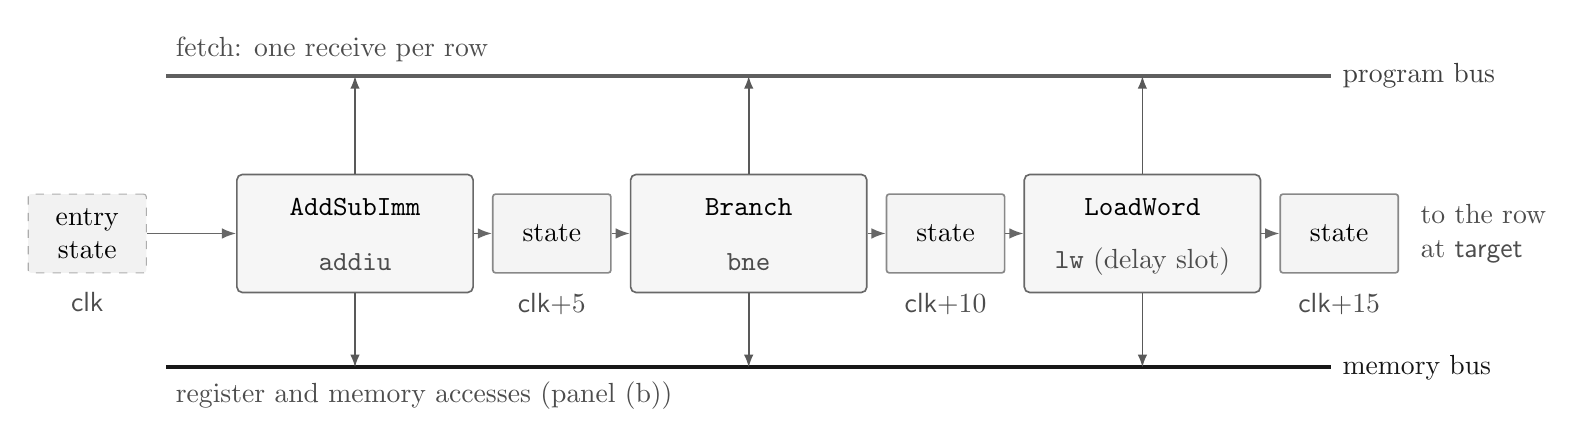
\begin{tikzpicture}[
  font=\large,
  unit/.style={rectangle, rounded corners=2pt, draw=zirenblue!85, line width=0.6pt,
               minimum width=3.0cm, minimum height=1.5cm, fill=zirenblue!5, align=center},
  reg/.style={rectangle, rounded corners=1pt, draw=zirenteal!85, line width=0.6pt,
              minimum width=1.5cm, minimum height=1.0cm, fill=zirenteal!8, align=center,
              font=\normalsize},
  pub/.style={rectangle, rounded corners=1pt, draw=zirenslate!80, dashed,
              minimum width=1.5cm, minimum height=1.0cm, fill=zirenlight, align=center,
              font=\normalsize},
  pbus/.style={line width=1.4pt, zirenblue!90},
  mbus/.style={line width=1.4pt, zirenorange!90!black},
  sig/.style={-{Latex[length=1.8mm]}, line width=0.6pt, zirenteal!90!black},
  tap/.style={-{Latex[length=1.6mm]}, line width=0.6pt, black!65},
  lbl/.style={font=\normalsize, black!70},
  hdr/.style={font=\normalsize\bfseries},
]
% ---------- the two shared buses
\draw[pbus] (-2.4,2.0) -- (12.4,2.0)
  node[right, font=\normalsize, text=zirenblue!80!black] {program bus};
\draw[mbus] (-2.4,-1.7) -- (12.4,-1.7)
  node[right, font=\normalsize, text=zirenorange!80!black] {memory bus};

% ---------- three opcode rows
\node[unit] (u1) at (0,0)    {};
\node[unit] (u2) at (5,0)    {};
\node[unit] (u3) at (10,0)   {};
\node[hdr] at ($(u1.north)+(0,-0.42)$) {\texttt{AddSubImm}};
\node[hdr] at ($(u2.north)+(0,-0.42)$) {\texttt{Branch}};
\node[hdr] at ($(u3.north)+(0,-0.42)$) {\texttt{LoadWord}};
\node[lbl] at ($(u1.south)+(0,0.40)$) {\texttt{addiu}};
\node[lbl] at ($(u2.south)+(0,0.40)$) {\texttt{bne}};
\node[lbl] at ($(u3.south)+(0,0.40)$) {\texttt{lw} (delay slot)};

% ---------- each row fetches from the program ROM and touches the memory bus
\foreach \u in {u1,u2,u3} {
  \draw[tap] (\u.north) -- (\u.north |- 0,2.0);
  \draw[tap] (\u.south) -- (\u.south |- 0,-1.7);
}
\node[lbl, anchor=south west] at (-2.4,2.06) {fetch: one receive per row};
\node[lbl, anchor=north west] at (-2.4,-1.76) {register and memory accesses (panel (b))};

% ---------- the state chain
\node[pub] (s0) at (-3.4,0) {entry\\state};
\node[reg] (s1) at (2.5,0)  {state};
\node[reg] (s2) at (7.5,0)  {state};
\node[reg] (s3) at (12.5,0) {state};
\draw[sig] (s0) -- (u1.west);
\draw[sig] (u1.east) -- (s1);
\draw[sig] (s1) -- (u2.west);
\draw[sig] (u2.east) -- (s2);
\draw[sig] (s2) -- (u3.west);
\draw[sig] (u3.east) -- (s3);
\node[lbl, anchor=north, align=center] at ($(s1.south)+(0,-0.12)$) {$\mathsf{clk}{+}5$};
\node[lbl, anchor=north, align=center] at ($(s2.south)+(0,-0.12)$) {$\mathsf{clk}{+}10$};
\node[lbl, anchor=north, align=center] at ($(s3.south)+(0,-0.12)$) {$\mathsf{clk}{+}15$};
\node[lbl, anchor=north, align=center] at ($(s0.south)+(0,-0.12)$) {$\mathsf{clk}$};
\node[lbl, anchor=west, align=left] at ($(s3.east)+(0.15,0)$) {to the row\\at $\mathsf{target}$};
\end{tikzpicture}
}
\caption{The state chain across three consecutive cycles. Each row receives the machine state of its cycle from the register on its left and sends that of the next to the register on its right, fetches its instruction from the preprocessed \texttt{Program} ROM on the program bus, and places its accesses on the memory bus.}
\label{fig:frame-flow}
\end{subfigure}

\vspace{0.7em}
\begin{subfigure}{0.76\textwidth}
\centering
\resizebox{\textwidth}{!}{% Panel (b) of the instruction frame: ONE row enlarged, showing the four fixed
% sub-cycle access positions.  A narrow canvas, so it scales up rather than down
% and its pin labels are the largest text in the figure.  The pins sit ON the
% row's lower edge with their labels BELOW it, so they cannot collide with the
% datapath lines inside the box.
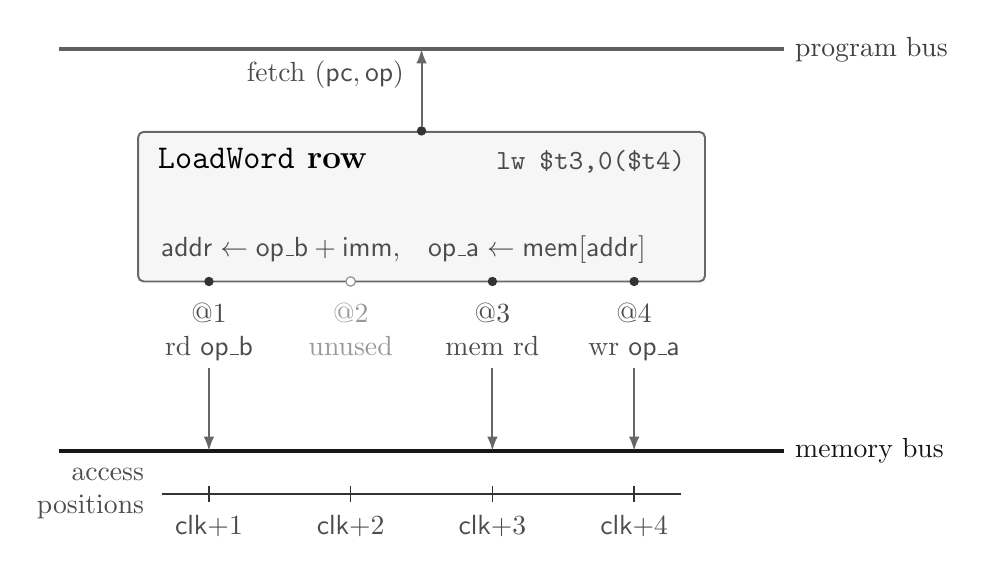
\begin{tikzpicture}[
  font=\large,
  chip/.style={rectangle, rounded corners=2pt, draw=zirenblue!85, line width=0.7pt,
               minimum width=7.2cm, minimum height=1.9cm, fill=zirenblue!5},
  mbus/.style={line width=1.6pt, zirenorange!90!black},
  pbus/.style={line width=1.6pt, zirenblue!90},
  wire/.style={line width=0.5pt, black!80},
  sig/.style={-{Latex[length=1.8mm]}, line width=0.7pt, zirenteal!90!black},
  pin/.style={circle, fill=black!80, inner sep=0pt, minimum size=3.4pt},
  npin/.style={circle, draw=black!45, fill=white, inner sep=0pt, minimum size=3.4pt},
  lbl/.style={font=\normalsize, black!70},
  hdr/.style={font=\large\bfseries},
]
% ---------- the row itself (spans y = -0.95 .. 0.95)
\node[chip] (u) at (0,0) {};
\node[hdr, anchor=north west] at ($(u.north west)+(0.14,-0.10)$) {\texttt{LoadWord} row};
\node[lbl, anchor=north east] at ($(u.north east)+(-0.14,-0.12)$) {\texttt{lw \$t3,0(\$t4)}};
\node[lbl, align=left, anchor=south west] at ($(u.south west)+(0.18,0.12)$)
  {$\mathsf{addr} \leftarrow \mathsf{op\_b} + \mathsf{imm}$,\quad
   $\mathsf{op\_a} \leftarrow \mathsf{mem}[\mathsf{addr}]$};

% ---------- fetch, upward to the program bus
\draw[pbus] (-4.6,2.0) -- (4.6,2.0)
  node[right, font=\normalsize, text=zirenblue!80!black] {program bus};
\node[pin] (uf) at (u.north) {};
\draw[sig] (uf) -- (u.north |- 0,2.0);
\node[lbl, anchor=south east] at ($(uf)+(-0.1,0.42)$) {fetch $(\mathsf{pc},\mathsf{op})$};

% ---------- the four access positions, pinned to the lower edge
\draw[mbus] (-4.6,-3.1) -- (4.6,-3.1)
  node[right, font=\normalsize, text=zirenorange!80!black] {memory bus};
\foreach \k/\t in {1/{rd $\mathsf{op\_b}$},2/{},3/{mem rd},4/{wr $\mathsf{op\_a}$}} {
  \pgfmathsetmacro{\px}{-2.7+1.8*(\k-1)}
  \ifx\t\empty
    \node[npin] (p\k) at (\px,-0.95) {};
    \node[lbl, anchor=north, align=center, black!40] at (\px,-1.10) {@\k\\ unused};
  \else
    \node[pin] (p\k) at (\px,-0.95) {};
    \node[lbl, anchor=north, align=center] at (\px,-1.10) {@\k\\ \t};
    \draw[sig] (\px,-2.05) -- (\px,-3.1);
  \fi
}

% ---------- the sub-cycle ruler under the bus
\draw[wire] (-3.3,-3.65) -- (3.3,-3.65);
\foreach \k in {1,...,4} {
  \pgfmathsetmacro{\px}{-2.7+1.8*(\k-1)}
  \draw[wire] (\px,-3.55) -- (\px,-3.75);
  \node[lbl, anchor=north] at (\px,-3.79) {$\mathsf{clk}{+}\k$};
}
\node[lbl, anchor=east, align=right] at (-3.4,-3.65) {access\\positions};
\end{tikzpicture}
}
\caption{One row enlarged: the four fixed sub-cycle access positions. Filled pins are accesses the opcode uses, hollow pins are unused.}
\label{fig:frame-chip}
\end{subfigure}
\caption{The instruction frame binds consecutive opcode rows into one state chain (panel~\subref{fig:frame-flow}) while assigning register and memory accesses to fixed sub-cycle positions (panel~\subref{fig:frame-chip}). The state tuple is $(\mathsf{shard}, \mathsf{clk}, \mathsf{pc}, \mathsf{next\_pc})$; the program tuple received from the ROM is $(\mathsf{pc}, \mathsf{opcode}, \mathsf{op\_a}, \mathsf{op\_b}, \mathsf{op\_c}, \mathsf{imm}, \ldots)$; each memory access sends the previous tuple $(\mathsf{shard},\, \mathsf{clk}{+}\mathsf{pos},\, \mathsf{addr},\, \mathsf{value})$ and receives the new one. In panel~\subref{fig:frame-flow} the \texttt{LoadWord} row sits in the branch's delay slot, so its successor arrives through the state register as the branch target rather than $\mathsf{pc}{+}4$. The rows compute $\mathsf{op\_a} \leftarrow \mathsf{op\_b} + \mathsf{imm}$ with a byte-checked result and witnessed carries (\texttt{AddSubImm}), $\mathsf{taken} \leftarrow [\mathsf{op\_b} \neq \mathsf{op\_c}]$ with $\mathsf{next\_next\_pc} \leftarrow \mathsf{taken}\,?\,\mathsf{target} : \mathsf{next\_pc}{+}4$ (\texttt{Branch}), and the aligned four-lane load of panel~\subref{fig:frame-chip} (\texttt{LoadWord}).}
\label{fig:frame}
\end{figure}

\subsection{Registers and memory}
\label{sec:air-memory}

Registers and memory share one offline memory-checking argument~\citep{blum1994} in the multiset style used by SP1~\citep{sp1}: the state of address $a$ is the tuple $(\mathsf{shard}, \mathsf{clk}, a, \mathsf{value})$ of its last access. An access at time $(s, c)$ \emph{sends} the previous tuple $(s', c', a, v')$ and \emph{receives} the new tuple $(s, c, a, v)$ on the \emph{memory} bus, with $v = v'$ for a read. The multiset balances if and only if every access consumes exactly the tuple produced by the previous access to the same address, provided timestamps strictly increase along each address's chain; the AIR of every access enforces $(s', c') < (s, c)$ by witnessing $c - c' - 1$, or $s - s' - 1$ when the shards differ, in range-checked limbs that cover a $\mathsf{clk} + \mathsf{pos}$ timestamp under a 25-bit clock fence, as a 16-bit limb and a 10-bit high limb (a one-bit \texttt{compare\_clk} selector chooses the branch). Words are four byte columns; the argument carries them as such.
Figure~\ref{fig:memchain} follows one address through two shards: which of its
tuples the memory bus balances, which are left to the cross-shard digest, and
where the chain begins and ends.

\begin{lemma}[Memory argument]
\label{lem:memory}
In a valid shard, for every address $a$ the accesses to $a$ form a chain ordered by $(\mathsf{shard}, \mathsf{clk})$ in which each access consumes exactly the tuple produced by the previous access to $a$, starting from the tuple supplied by the initial-state row of $a$ and ending at the tuple consumed by its final-state row; in particular every read returns the value of the last write.
\end{lemma}
\begin{proof}
Each access sends its previous tuple and receives its new tuple on the memory bus, and its constraints enforce that the new timestamp strictly exceeds the previous one. Balance of the memory bus, restricted to the tuples with address $a$, gives a graph as in Lemma~\ref{lem:chain} with the initial-state row as source and the final-state row as sink; strictly increasing timestamps exclude cycles, so the accesses form one path, and along the path a read carries its previous value forward unchanged.
\end{proof}

\paragraph{Registers.} The \texttt{MemoryBump} chip inserts, for every register at its first touch in a shard, a shadow read at $(\mathsf{shard}, 0)$. Since $\mathsf{clk}$ restarts at zero in every shard and real accesses sit at positions $1..4$ of a tick, the previous access of a register is always in the current shard. The register variant of the access columns therefore drops $\mathsf{prev\_shard}$, the compare selector and one limb, which is re-derived linearly from the others: 10 columns become 7 on every register access of every instruction.

\paragraph{Shard-local memory.} Within a shard, the first access to a word must consume a tuple that no access in the shard produced, and the last access produces a tuple that nothing in the shard consumes. The \texttt{MemoryLocal} chip records, for every word touched in the shard, its initial and final $(\mathsf{shard}, \mathsf{clk}, \mathsf{value})$; it sends the initial tuple on the memory bus (so the first access can consume it) and receives the final one, and it forwards both as \emph{global} interactions (Section~\ref{sec:air-global}) so that they are matched across shards. On a \texttt{reth} block (the Ethereum execution-client workload of Section~\ref{sec:performance}) a few hundred thousand words are touched per shard, most of them the hot working set touched again in the next shard; the two global rows per touched word are the largest single contribution to trace area, which is why the shard size matters (Section~\ref{sec:performance}).

\paragraph{Whole-execution memory.} \texttt{MemoryGlobalInit} carries the memory's initial contents (the program image and the hint data written into untouched words) and \texttt{MemoryGlobalFinalize} its final contents. Both witness the word as 32 boolean columns, which is what makes every value that enters memory byte-shaped by construction; addresses are 32-bit decomposed and proved strictly increasing along the table through a running comparison against the previous address, with the address cursors published as public values so the recursion can check that consecutive tables tile the address space without overlap. The program image itself is bound by the verifying key: its digest (Section~\ref{sec:air-global}) is a public parameter, and the init table must consume it.

\paragraph{What is byte-checked.} Every value that enters a register is byte-checked by the frame at the write, and every value a precompile writes to memory is byte-checked or bit-decomposed by the precompile chip; memory-instruction rows therefore omit the two additional byte lookups per word that accesses otherwise carry.

\begin{figure}[!tbp]
\centering
\resizebox{\textwidth}{!}{% The memory argument for ONE address: a chain that is shard-local on the
% memory bus and closed across shards only by the septic digest.  Solid edges
% are memory-bus tuples, dashed edges are global interactions.  The two shards
% are stacked rather than placed side by side, so that the canvas stays close
% to 2:1 and the tuple labels survive scaling to \textwidth.
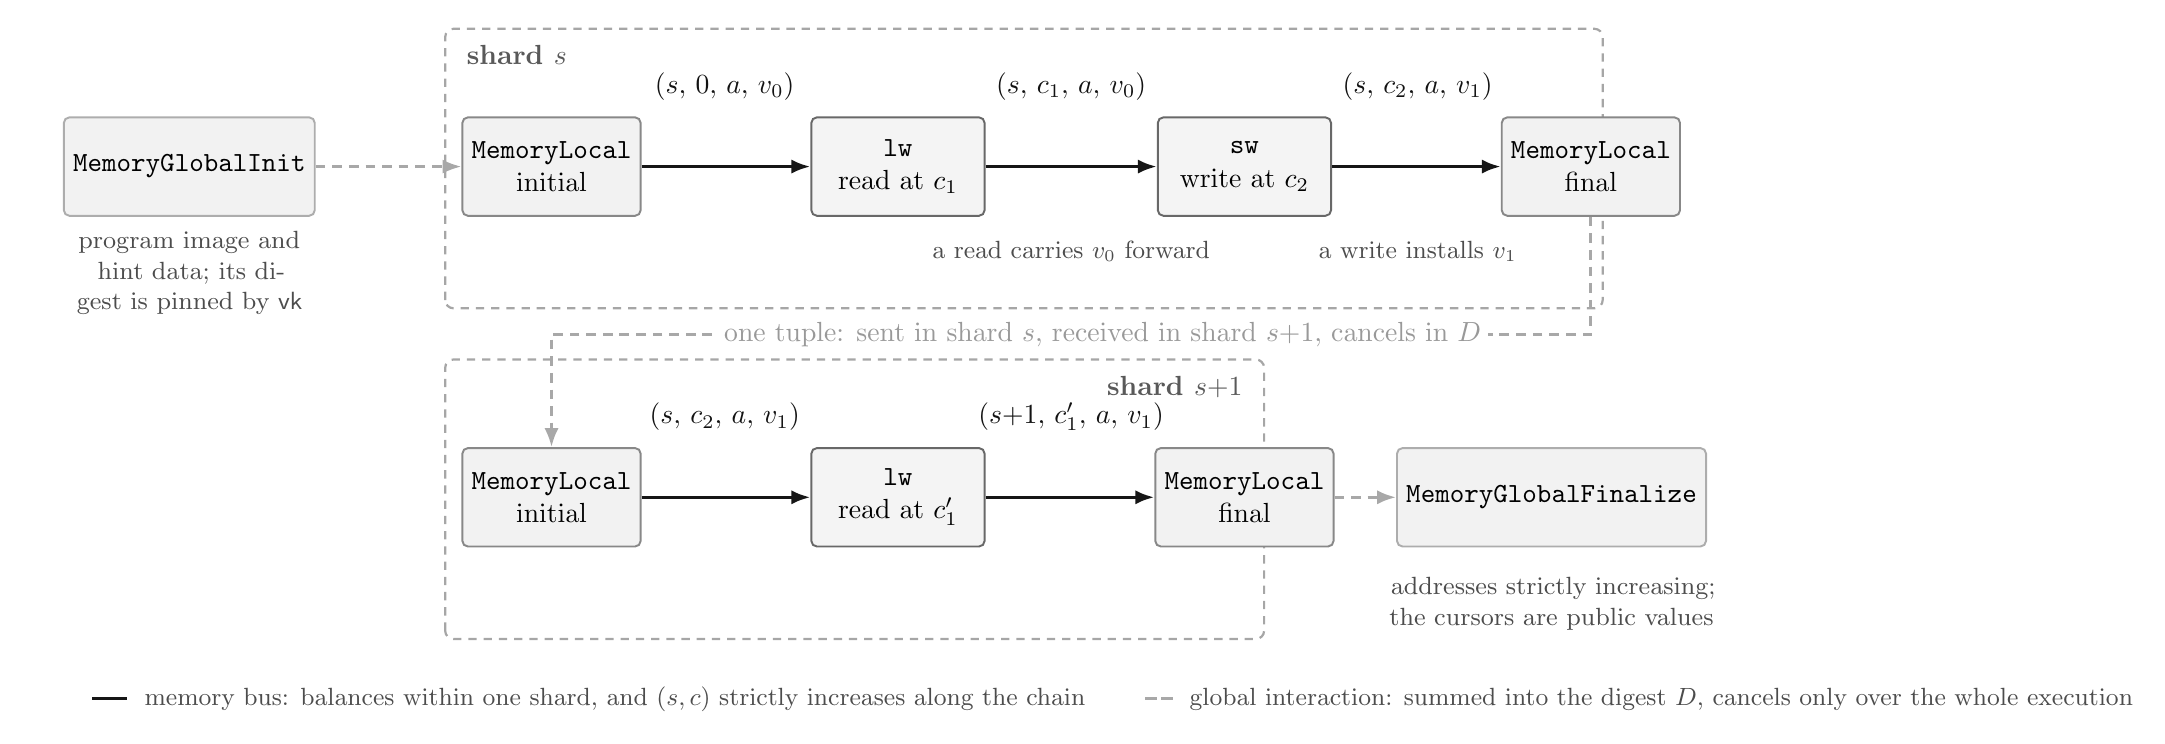
\begin{tikzpicture}[
  font=\large,
  acc/.style={rectangle, rounded corners=2pt, draw=zirenblue!85, fill=zirenblue!6,
              line width=0.7pt, minimum width=2.2cm, minimum height=1.25cm,
              align=center, font=\normalsize},
  loc/.style={rectangle, rounded corners=2pt, draw=zirenteal!85, fill=zirenteal!9,
              line width=0.7pt, minimum width=2.2cm, minimum height=1.25cm,
              align=center, font=\normalsize},
  glob/.style={rectangle, rounded corners=2pt, draw=zirenslate!80, fill=zirenlight,
               line width=0.7pt, minimum width=2.4cm, minimum height=1.25cm,
               align=center, font=\normalsize},
  bus/.style={-{Latex[length=2.4mm]}, line width=1.2pt, zirenorange!85!black},
  gl/.style={-{Latex[length=2.4mm]}, line width=1.1pt, zirenslate!85, dashed,
             dash pattern=on 3.5pt off 2.5pt},
  tup/.style={font=\normalsize, text=zirenorange!70!black, inner sep=1.5pt},
  gtup/.style={font=\normalsize, text=zirenslate, align=center, inner sep=2.5pt,
               fill=white},
  note/.style={font=\small, black!70, align=center, inner sep=1.5pt},
  hdr/.style={font=\normalsize\bfseries, black!65},
  shardbox/.style={rectangle, rounded corners=3pt, draw=black!35, dashed,
                   dash pattern=on 3pt off 2.5pt, line width=0.8pt},
]

% ================= shard s: the memory bus balances inside this box
\draw[shardbox] (-1.35,-1.8) rectangle (13.35,1.75);
\node[hdr, anchor=north west] at (-1.2,1.66) {shard $s$};

\node[loc] (li) at (0,0)    {\texttt{MemoryLocal}\\initial};
\node[acc] (r1) at (4.4,0)  {\texttt{lw}\\read at $c_1$};
\node[acc] (w1) at (8.8,0)  {\texttt{sw}\\write at $c_2$};
\node[loc] (lf) at (13.2,0) {\texttt{MemoryLocal}\\final};

\draw[bus] (li) -- (r1);
\draw[bus] (r1) -- (w1);
\draw[bus] (w1) -- (lf);
\node[tup] at (2.2,1.02)  {$(s,\,0,\,a,\,v_0)$};
\node[tup] at (6.6,1.02)  {$(s,\,c_1,\,a,\,v_0)$};
\node[tup] at (11.0,1.02) {$(s,\,c_2,\,a,\,v_1)$};
\node[note] at (6.6,-1.08) {a read carries $v_0$ forward};
\node[note] at (11.0,-1.08) {a write installs $v_1$};

% ================= shard s+1: the chain resumes at the tuple shard s left
\draw[shardbox] (-1.35,-6.0) rectangle (9.05,-2.45);
\node[hdr, anchor=north east] at (8.9,-2.54) {shard $s{+}1$};

\node[loc] (li2) at (0,-4.2)   {\texttt{MemoryLocal}\\initial};
\node[acc] (r2)  at (4.4,-4.2) {\texttt{lw}\\read at $c_1'$};
\node[loc] (lf2) at (8.8,-4.2) {\texttt{MemoryLocal}\\final};

\draw[bus] (li2) -- (r2);
\draw[bus] (r2) -- (lf2);
\node[tup] at (2.2,-3.18) {$(s,\,c_2,\,a,\,v_1)$};
\node[tup] at (6.6,-3.18) {$(s{+}1,\,c_1',\,a,\,v_1)$};

% ================= the same tuple, forwarded as two global interactions
\draw[gl] (lf.south) -- (13.2,-2.13) -- (0,-2.13) -- (li2.north);
\node[gtup] at (7.0,-2.13)
  {one tuple: sent in shard $s$, received in shard $s{+}1$, cancels in $D$};

% ================= the whole-execution tables at the two ends of the chain
\node[glob] (gi) at (-4.6,0)    {\texttt{MemoryGlobalInit}};
\node[glob] (gf) at (12.7,-4.2) {\texttt{MemoryGlobalFinalize}};
\draw[gl] (gi) -- (li);
\draw[gl] (lf2) -- (gf);
\node[note, text width=4.0cm] at (-4.6,-1.35)
  {program image and hint data; its digest is pinned by $\mathsf{vk}$};
\node[note, text width=4.2cm] at (12.7,-5.55)
  {addresses strictly increasing; the cursors are public values};

% ================= legend
\node[note, anchor=north west, align=left] at (-5.9,-6.55)
  {\textcolor{zirenorange!85!black}{\rule[0.22em]{1.4em}{1.1pt}}\ \
   memory bus: balances within one shard, and $(s,c)$ strictly increases
   along the chain \qquad
   \textcolor{zirenslate!85}{\rule[0.22em]{0.45em}{1.1pt}\hspace{0.18em}%
   \rule[0.22em]{0.45em}{1.1pt}}\ \
   global interaction: summed into the digest $D$, cancels only over the whole
   execution};
\end{tikzpicture}
}
\caption{The chain of one address $a$ across a shard boundary. A shard proof can balance only the tuples whose two sides it contains, so the \texttt{MemoryLocal} rows stand in for the accesses it cannot see: the initial row supplies the tuple the shard's first access consumes, and the final row consumes the tuple its last access produces. Those two tuples are then the \emph{same} tuple on either side of the boundary, carried with opposite signs into the digest $D$ of Section~\ref{sec:air-global}, which is why the chain closes over the execution without any shard proof depending on another. The two ends belong to the whole-execution tables rather than to a shard.}
\label{fig:memchain}
\end{figure}

\subsection{Cross-shard interactions: the global digest}
\label{sec:air-global}

Interactions whose two sides live in different shards cannot be balanced by a per-shard fraction sum. These include the initial and final tuples of every shard-touched word, memory initialisation and finalisation, and syscall pairings. \Zirenver{} carries them in an elliptic-curve digest of the kind SP1 introduced~\citep{sp1}. An interaction tuple $\bm m \in \F^7$ is mapped to a point of $E: y^2 = x^3 + 3\zeta x - 3$ over the degree-seven extension $\F_{p^7} = \F[\zeta]/(\zeta^7 + 2\zeta - 8)$; sends contribute the point and receives its negation, and the sum over the whole execution must be the identity. A shard proof publishes its running sum, and the block verifier adds them.

The \texttt{Global} chip has one row per such interaction. It witnesses the point, checks the curve equation, and fixes the sign of $y$ by confining its top limb to one of two disjoint bands, one for sends and one for receives. The running sum is carried on an accumulation bus, row $i$ receiving $(i, S_i)$ and sending $(i+1, S_{i+1})$ with the chord identities enforcing the addition, and the public-values table closes the chain.

The two exceptional cases of the chord law are excluded separately, and by different mechanisms. Both identities carry the factor $(x_2 - x_1)$:
\[
  C_x = (x_1 + x_2 + x_3)(x_2 - x_1)^2 - (y_2 - y_1)^2, \qquad
  C_y = (y_1 + y_3)(x_2 - x_1) - (y_2 - y_1)(x_1 - x_3).
\]
At $P_2 = -P_1$ we have $C_x = -4y_1^2$, which is non-zero whenever $y_1 \neq 0$, so the identity case is rejected by $C_x$ itself. At $P_2 = P_1$ both coordinate differences vanish, so $C_x$ and $C_y$ hold for \emph{every} $P_3$ and the identities alone would leave the next running sum unconstrained but for the curve equation. The chip therefore witnesses $(x_2 - x_1)^{-1}$ and constrains $(x_2 - x_1)\cdot(x_2-x_1)^{-1} = 1$ on every real row, which makes $x_2 \neq x_1$ a constraint rather than an assumption; since both points are on the curve, $x_2 = x_1$ forces $y_2 \in \{y_1, -y_1\}$ and there is no third case. The first row is separately safe: the sum starts at a fixed public offset point $D$ chosen with $\pm D$ outside the image of the map. What remains is a running sum at some later row coinciding with the next interaction's point, which the inverse makes unprovable rather than unconstrained, and whose probability Assumption~\ref{ass:digest} bounds by the unquantified $\varepsilon_{\mathrm{digest}}$.

One departure from SP1 matters. SP1 hashes the message to the curve with a permutation constrained inside the chip, so its points are random-oracle outputs. \Zirenver{} applies no hash: the message \emph{is} the $x$-coordinate, up to a prover-chosen byte $\mathsf{offset}$ in the low positions of $x_6$ that makes the curve's right-hand side a square, so that a point with that $x$ exists. That is what reduces the chip from a few hundred columns to a few dozen, and it changes the security argument rather than merely its constants.

\subsection{Security of the digest}
\label{sec:air-digest-security}

The lift is a map on \emph{pairs}, not on messages: $\mathsf{enc}(\bm m, \mathsf{offset})$. The offset is a witness column, and the chip constrains only that it is a byte occupying the low positions of $x_6$; it does not constrain it to be canonical. The honest prover takes the smallest admissible offset. The implementation scans $\mathsf{offset} = 0, \dots, 255$ and stops at the first value whose $x$ makes $x^3 + 3\zeta x - 3$ a square in $\F_{p^7}$, so that the point exists. Minimality is not an AIR constraint, so a satisfying trace may carry any admissible offset. We therefore write $\mathcal P$ for the \emph{reachable pairs} $(\bm m, \mathsf{offset})$ that an interaction of a satisfying trace can carry, given the range facts each sending chip enforces and the byte bound on the offset, and reserve $\mathcal M$ for the projection of $\mathcal P$ onto messages. $\mathcal M$ is far smaller than $\F^7$, since every limb of a memory or syscall tuple is a byte, a bounded clock limb or a bounded address, and the whole argument rests on that; the offset multiplies the reachable set by at most $256$.

Two consequences follow from the offset being free. First, cancellation is over pairs: a send and its matching receive contribute $\pm\mathsf{enc}(\bm m, \mathsf{offset})$ and cancel only if they agree on the offset. A trace whose two sides choose different admissible offsets for the same message does not balance and is rejected; the freedom costs completeness, not soundness, on that axis. Second, and this is the axis that matters below, the adversary searching for a vanishing combination searches over $\mathcal P$ rather than $\mathcal M$.

\begin{lemma}[injectivity of the lift]
\label{lem:digest}
Assume the message limbs satisfy the range facts the sending chips enforce, so that $256\,m_6 + \mathsf{offset} < p$. Then $\mathsf{enc}$ is injective: limbs $x_0, \dots, x_5$ are $m_0, \dots, m_5$; $x_6$ is $m_6$ shifted above a low byte holding the offset, which the bound makes separable; and the two sign bands are disjoint. So $\bm m$ and the offset are recoverable from the point.
\end{lemma}

Injectivity makes the digest a faithful encoding of the multiset of \emph{pairs}, but it is not what makes the argument sound. If a claimed execution has send and receive multisets $S \neq R$ over $\mathcal P$ whose digests agree, then $\sum_i c_i\,\mathsf{enc}(\bm m_i, \mathsf{offset}_i) = O$ for the non-zero integer vector $c = \mathrm{mult}_S - \mathrm{mult}_R$. Equality of encoded multisets implies equality of message multisets only after projecting away the offsets, which is legitimate precisely because the lift is injective on pairs (Lemma~\ref{lem:digest}). Soundness is therefore exactly:

\begin{assumption}[no reachable vanishing combination]
\label{ass:digest}
Let $\lambda$ be the security parameter, let $N_{\mathrm{int}}$ bound the interactions a block proof may contain and $B$ the per-interaction multiplicity bound, and let $\mathcal P$ be the reachable pairs above. For every adversary $\mathcal A$ running in time at most $T(\lambda)$ and making at most $q(\lambda)$ queries to the hash functions of the protocol,
\[
  \Pr\big[\, \mathcal E(\mathcal A) \,\big] \;\le\; \varepsilon_{\mathrm{digest}}(\lambda, T, q, N_{\mathrm{int}}, B),
\]
where $\mathcal E(\mathcal A)$ is the event that $\mathcal A$ outputs reachable pairs $\{(\bm m_i, \mathsf{offset}_i)\}_{i \le N_{\mathrm{int}}} \subseteq \mathcal P$ together with a non-zero integer vector $c \in \mathbb{Z}^{N_{\mathrm{int}}}$ satisfying $\|c\|_\infty \le B$ and $\sum_i c_i\, \mathsf{enc}(\bm m_i, \mathsf{offset}_i) = O$ in $E(\F_{p^7})$.
\end{assumption}
The assumption is that $\varepsilon_{\mathrm{digest}}$ is at most the level Section~\ref{sec:iopp-soundness} targets, at the interaction and multiplicity bounds of a block proof; that is what Theorem~\ref{thm:composition} takes as a hypothesis, and this machine's parameters are fixed rather than a family, so the statement is concrete. We do not claim a value for it; the paragraph below explains why, and Section~\ref{sec:iopp-soundness} carries it as a named open component rather than folding it into a bit total.

This is the weakest link in the accounting, and we state it rather than a bit figure for two reasons. Hashing to the curve, as SP1 does, would make the points random-oracle outputs and support a clean discrete-logarithm statement about points no adversary can steer. Here the prover chooses points from a structured set, and reads a message off any target $x$-coordinate by inverting the limb layout of Lemma~\ref{lem:digest}; the uncanonicalised offset widens that set by a further factor of at most $256$. The sparsity of $\mathcal P$ blocks the obvious attack of choosing a generator $G$, selecting scalars that sum to zero and reading their $x$-coordinates as messages, since almost no such $x$ has the limb shape a reachable pair requires. This reasoning depends on every sending chip bounding every contributed limb, an arithmetisation obligation not collected in one certificate today. Sparsity also does not yield a bit estimate: the relevant generalised-birthday cost falls with the number of lists and must be bounded using the interactions a prover can place in a trace, not only $|E(\F_{p^7})| \approx 2^{217}$. That analysis remains open. Section~\ref{sec:iopp-soundness} therefore lists the digest as a separate computational component.

\subsection{Trace uniqueness}
\label{sec:air-unique}

\begin{theorem}[From chip determinism to trace uniqueness]
\label{thm:unique}
Fix a program image, public values and a valid shard. If every chip of the shard is deterministic in the sense of Definition~\ref{def:det}, then the rows reachable from the entry state along the state and memory buses are determined by the program image and the public values: any two valid shards with the same program image and public values agree on those rows up to permutation.
\end{theorem}
\begin{proof}
By Lemma~\ref{lem:chain} the instruction rows of either shard form one chain from the entry state; write $r_1, \dots, r_N$ for the first shard's chain. We show by induction on $i$ that $r_i$ has the same inputs and outputs in both shards. The inputs of $r_i$ are its received state tuple $s_{i-1}$, its fetched instruction, and the previous values of the addresses it accesses. $s_0$ is public and $s_{i-1}$ is the output of $r_{i-1}$ by induction. The fetched instruction is a function of $\mathsf{pc}(s_{i-1})$ because the program bus is received only by the preprocessed program table, which is committed. The previous value of an address is, by Lemma~\ref{lem:memory}, the value written by the last earlier access to that address, or the initial value from the memory-initialisation table, which is bound to the program image and the public address cursors; earlier accesses belong to rows $r_j$, $j < i$, whose outputs agree by induction. So the inputs of $r_i$ agree, and determinism of its chip gives that its outputs agree. Rows of non-instruction chips (the memory-initialisation and finalisation tables, the shadow reads, the digest rows, the tables) are determined in the same way from the bus tuples they receive, which are outputs of instruction rows or public. Rows that participate in no bus reachable from the entry state are not covered by this argument; the arithmetisation admits none, because every real row carries a frame or a memory access, but that is a property of the chip set rather than of the buses, and we do not prove it here.
\end{proof}

The theorem is stated, not machine-checked; its premises are the chip-level determinism statements, of which \ndetproved{} of \ndettotal{} are machine-checked today and the rest are assumed (Section~\ref{sec:verification-det}), and the two bus lemmas are the standard arguments of the multiset construction.

\subsection{Preprocessed tables}

The \texttt{Byte} table has $2^{16}$ rows indexed by a byte pair and one multiplicity column per operation (bitwise operations, shifts, comparisons and 8/16-bit range checks); every carry, borrow, comparison and range check in the machine is an interaction with it. The \texttt{Range} table serves the clock limbs, and the \texttt{Program} table holds the decoded program image. Preprocessed tables are committed at setup as part of the verifying key and opened at the same points as the main trace.

\subsection{The shard-level lookup argument}
\label{sec:air-logup}

This is the bus argument of \S\ref{sec:argument-components}.

One \LogUp{} instance proves all interactions of a shard on the program, state, memory, byte, range, syscall, global and accumulation buses. After committing the trace, the verifier samples $\alpha, \beta \in \EF$. Every interaction $(\mathsf{bus}, \bm f, m)$ contributes $m / (\alpha - \mathsf{bus} - \sum_{j \ge 1} \beta^{j} f_j)$, and the prover shows that sends and receives have equal sums. These fractions are leaves of a layered GKR circuit. Sumcheck proves its transitions from the root down, and the final layer produces multilinear evaluation claims on the participating columns for the polynomial commitment. A reth shard has on the order of $10^8$ leaves. Section~\ref{sec:performance} shows that this circuit is the largest GPU-kernel consumer; its leaf count is the number of (row, interaction) pairs, so interactions per row are a separate cost from columns.

Soundness of the fraction identity is $\deg/|\EF|$ per sumcheck round plus the collision probability of the fingerprint, which grows with the number of leaves; Section~\ref{sec:iopp-soundness} lists it as one component of the accounting. The checked-in schedule grinds the \LogUp{} challenge by 16 bits (Table~\ref{tab:whir-schedule}); the performance baseline of Section~\ref{sec:perf-changes} was measured with none (\S\ref{sec:iopp-soundness}).

\subsection{The shard-level zerocheck}
\label{sec:air-zerocheck}

This is the constraint argument of \S\ref{sec:argument-components}.

The polynomial constraints of all chips are proved by \emph{one} zerocheck. The verifier samples $\tau$ for a random linear combination across chips and $\mu$ across the constraints of a chip; for each chip the polynomial $C_c(\bm X) = \sum_k \mu^k\, c_{c,k}(\text{row}(\bm X))$ must vanish on the chip's real rows. The prover proves $\sum_{\bm b} \eqf(\bm b, \bm r)\, \sum_c \tau^c C_c(\bm b) = 0$ for a random $\bm r$ by sumcheck over the tallest chip's variables, with shorter chips handled by an analytic ``virtual $\ge$'' factor rather than padding, and the final evaluation claims on the chips' columns are again handed to the commitment. The constraint degree is three, which fixes the degree of the round polynomials at four; the constraint-evaluation kernel on the GPU is compiled per chip from the same constraint description that the verifier uses, except for the widest accelerator chips, which are interpreted (Table~\ref{tab:census}), and a mismatch between the two is caught by host verification (Section~\ref{sec:performance}).

The zerocheck's claims are seeded from the \LogUp{} openings so that the two protocols share one opening of each column: after the two sumchecks, what remains is a set of (chip, column, point, value) claims, of the order of $3.6 \cdot 10^4$ per shard, and turning those into a single claim on a single committed polynomial is the job of the commitment layer.

\section{The jagged commitment}
\label{sec:pcs}

After the lookup argument and zerocheck, the verifier holds evaluation claims on individual chip columns. A shard of the \texttt{reth} workload has about $3.6 \cdot 10^4$ columns whose heights range from 32 rows to millions. Committing each column or chip separately would cost one Merkle root and query phase per commitment, and recursion would depend on the chip set of each shard. \Zirenver{} instead reduces all claims to one evaluation of a \emph{logical} dense polynomial and opens it once. The data may reside under several ordered input commitments, with the preprocessed round first and main round last, but one jagged reduction, one branching-program assist and one batched PCS opening cover all roots.

The property this buys is modularity in the sense of Section~\ref{sec:ipcore}: because the verifier of the reduction depends only on the logarithm of the committed area and on a fixed description of the column geometry, a chip can be widened, narrowed, added or removed without redesigning the layer above it. The block's internals can be revised, as they were four times in Section~\ref{sec:perf-changes}, while the reduction protocol remains the same.

\subsection{Input commitments, dense packing and stacking}
\label{sec:pcs-stacking}

Figure~\ref{fig:jagged} shows the two views this section connects: the ordered input rounds, each keeping its own root, and the single logical dense table that the reduction opens.

\begin{figure}[t]
\centering
\resizebox{\textwidth}{!}{% Figure 5: physical commitments, logical jagged reduction, and authenticated closing claims.
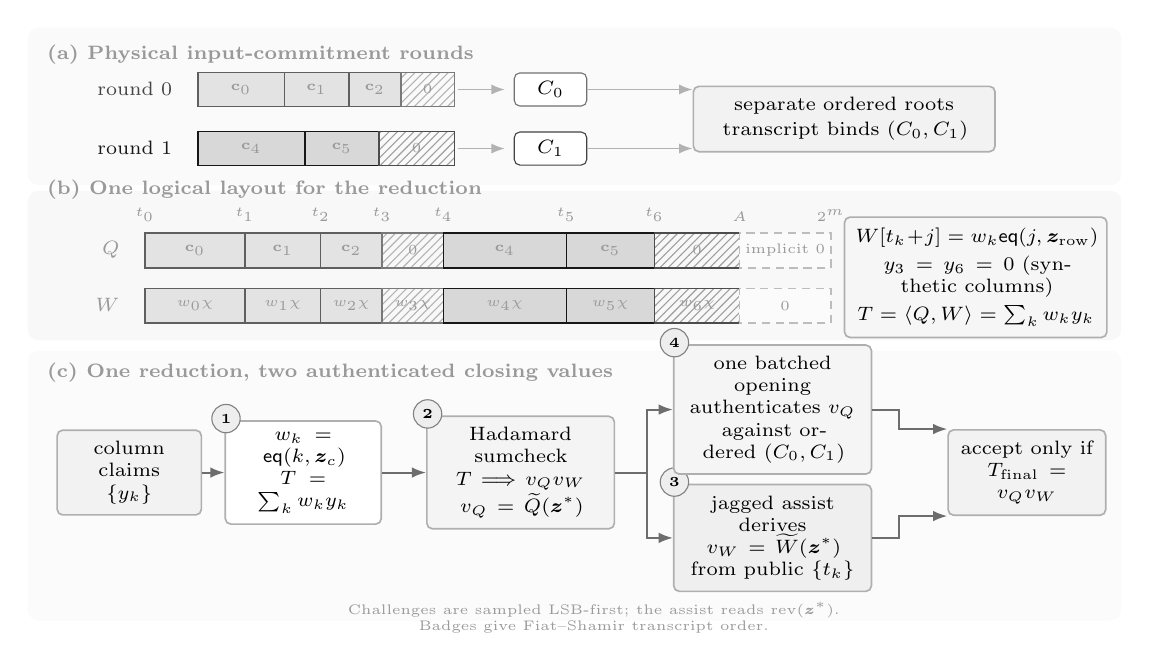
\begin{tikzpicture}[
  font=\scriptsize,
  cell0/.style={draw=zirenblue!90, fill=zirenblue!16, line width=0.55pt},
  cell1/.style={draw=zirenorange!90!black, fill=zirenorange!17, line width=0.55pt},
  pad0/.style={draw=zirenblue!75, fill=white, pattern=north east lines,
               pattern color=zirenblue!42, line width=0.55pt},
  pad1/.style={draw=zirenorange!78, fill=white, pattern=north east lines,
               pattern color=zirenorange!42, line width=0.55pt},
  implicit/.style={draw=zirenslate!65, densely dashed, fill=zirenslate!4, line width=0.55pt},
  box/.style={rectangle, rounded corners=2pt, draw=zirenslate!78, fill=white,
              align=center, minimum height=0.82cm, inner sep=4pt, line width=0.6pt},
  root/.style={rectangle, rounded corners=2pt, draw=zirenslate!80, fill=white,
               minimum width=0.92cm, minimum height=0.42cm, inner sep=2pt,
               font=\scriptsize\bfseries},
  badge/.style={circle, draw=zirenteal!90, fill=zirenteal!12,
                minimum size=0.36cm, inner sep=0pt, font=\tiny\bfseries},
  flow/.style={-{Latex[length=1.8mm]}, line width=0.7pt, zirenteal!95!black},
  bind/.style={-{Latex[length=1.7mm]}, line width=0.6pt, zirenslate!75},
  lab/.style={font=\scriptsize, text=zirenslate},
  tinylabel/.style={font=\tiny, text=zirenslate},
  panel/.style={font=\scriptsize\bfseries, text=zirenslate,
                anchor=north west, inner sep=0pt},
]

% (a) Physical input commitments.
\node[panel] at (-0.10,3.34) {(a) Physical input-commitment rounds};

\node[lab, anchor=east, text=zirenblue!90!black] at (1.62,2.78)
  {round 0};
\draw[cell0] (1.82,2.55) rectangle (2.92,2.98);
\draw[cell0] (2.92,2.55) rectangle (3.74,2.98);
\draw[cell0] (3.74,2.55) rectangle (4.40,2.98);
\draw[pad0]  (4.40,2.55) rectangle (5.08,2.98);
\node[tinylabel] at (2.37,2.765) {$\mathbf c_0$};
\node[tinylabel] at (3.33,2.765) {$\mathbf c_1$};
\node[tinylabel] at (4.07,2.765) {$\mathbf c_2$};
\node[tinylabel] at (4.74,2.765) {$0$};
\draw[bind] (5.12,2.765) -- (5.72,2.765);
\node[root, draw=zirenblue!80] (c0) at (6.30,2.765) {$C_0$};

\node[lab, anchor=east, text=zirenorange!90!black] at (1.62,2.03)
  {round 1};
\draw[cell1] (1.82,1.80) rectangle (3.18,2.23);
\draw[cell1] (3.18,1.80) rectangle (4.12,2.23);
\draw[pad1]  (4.12,1.80) rectangle (5.08,2.23);
\node[tinylabel] at (2.50,2.015) {$\mathbf c_4$};
\node[tinylabel] at (3.65,2.015) {$\mathbf c_5$};
\node[tinylabel] at (4.60,2.015) {$0$};
\draw[bind] (5.12,2.015) -- (5.72,2.015);
\node[root, draw=zirenorange!82] (c1) at (6.30,2.015) {$C_1$};

\node[box, text width=3.55cm, fill=zirenlight] (roots) at (10.03,2.39)
  {separate ordered roots\\[1pt]
   transcript binds $(C_0,C_1)$};
\draw[bind] (c0.east) -- (roots.west |- c0.east);
\draw[bind] (c1.east) -- (roots.west |- c1.east);

% (b) Aligned logical tables.
\node[panel] at (-0.10,1.62) {(b) One logical layout for the reduction};

\node[lab, anchor=east, font=\scriptsize\bfseries] at (0.95,0.73) {$Q$};
\draw[cell0] (1.15,0.50) rectangle (2.42,0.94);
\draw[cell0] (2.42,0.50) rectangle (3.38,0.94);
\draw[cell0] (3.38,0.50) rectangle (4.16,0.94);
\draw[pad0]  (4.16,0.50) rectangle (4.94,0.94);
\draw[cell1] (4.94,0.50) rectangle (6.50,0.94);
\draw[cell1] (6.50,0.50) rectangle (7.62,0.94);
\draw[pad1]  (7.62,0.50) rectangle (8.70,0.94);
\draw[implicit] (8.70,0.50) rectangle (9.86,0.94);
\node[tinylabel] at (1.785,0.72) {$\mathbf c_0$};
\node[tinylabel] at (2.90,0.72) {$\mathbf c_1$};
\node[tinylabel] at (3.77,0.72) {$\mathbf c_2$};
\node[tinylabel] at (4.55,0.72) {$0$};
\node[tinylabel] at (5.72,0.72) {$\mathbf c_4$};
\node[tinylabel] at (7.06,0.72) {$\mathbf c_5$};
\node[tinylabel] at (8.16,0.72) {$0$};
\node[tinylabel] at (9.28,0.72) {implicit $0$};

\node[tinylabel, anchor=south] at (1.15,0.97) {$t_0$};
\node[tinylabel, anchor=south] at (2.42,0.97) {$t_1$};
\node[tinylabel, anchor=south] at (3.38,0.97) {$t_2$};
\node[tinylabel, anchor=south] at (4.16,0.97) {$t_3$};
\node[tinylabel, anchor=south] at (4.94,0.97) {$t_4$};
\node[tinylabel, anchor=south] at (6.50,0.97) {$t_5$};
\node[tinylabel, anchor=south] at (7.62,0.97) {$t_6$};
\node[tinylabel, anchor=south] at (8.70,0.97) {$A$};
\node[tinylabel, anchor=south] at (9.86,0.97) {$2^m$};

\node[lab, anchor=east, font=\scriptsize\bfseries] at (0.95,0.03) {$W$};
\draw[cell0] (1.15,-0.20) rectangle (2.42,0.24);
\draw[cell0] (2.42,-0.20) rectangle (3.38,0.24);
\draw[cell0] (3.38,-0.20) rectangle (4.16,0.24);
\draw[pad0]  (4.16,-0.20) rectangle (4.94,0.24);
\draw[cell1] (4.94,-0.20) rectangle (6.50,0.24);
\draw[cell1] (6.50,-0.20) rectangle (7.62,0.24);
\draw[pad1]  (7.62,-0.20) rectangle (8.70,0.24);
\draw[implicit] (8.70,-0.20) rectangle (9.86,0.24);
\node[tinylabel] at (1.785,0.02) {$w_0\chi$};
\node[tinylabel] at (2.90,0.02) {$w_1\chi$};
\node[tinylabel] at (3.77,0.02) {$w_2\chi$};
\node[tinylabel] at (4.55,0.02) {$w_3\chi$};
\node[tinylabel] at (5.72,0.02) {$w_4\chi$};
\node[tinylabel] at (7.06,0.02) {$w_5\chi$};
\node[tinylabel] at (8.16,0.02) {$w_6\chi$};
\node[tinylabel] at (9.28,0.02) {$0$};

\node[box, text width=3.05cm, fill=zirenblue!5] at (11.70,0.38)
  {$W[t_k+j]=w_k\eqf(j,\bm z_{\mathrm{row}})$\\[2pt]
   $y_3=y_6=0$ (synthetic columns)\\[2pt]
   $T=\langle Q,W\rangle=\sum_kw_k y_k$};

% (c) Proof obligations after the reduction.
\node[panel] at (-0.10,-0.70) {(c) One reduction, two authenticated closing values};

\node[box, text width=1.55cm, fill=zirenlight] (claims) at (0.95,-2.10)
  {column claims\\$\{y_k\}$};

\node[box, text width=1.70cm] (mix) at (3.16,-2.10)
  {$w_k=\eqf(k,\bm z_c)$\\
   $T=\sum_kw_k y_k$};
\node[badge] at ($(mix.north west)+(0.02,0.02)$) {1};

\node[box, text width=2.10cm, fill=zirenblue!6] (sumcheck) at (5.92,-2.10)
  {Hadamard sumcheck\\
   $T\Longrightarrow v_Qv_W$\\
   $v_Q=\widetilde Q(\bm z^*)$};
\node[badge] at ($(sumcheck.north west)+(0.02,0.02)$) {2};

\node[box, text width=2.23cm, fill=zirenorange!7] (assist) at (9.12,-2.93)
  {jagged assist\\
   derives $v_W=\widetilde W(\bm z^*)$\\
   from public $\{t_k\}$};
\node[badge] at ($(assist.north west)+(0.02,0.02)$) {3};

\node[box, text width=2.23cm, fill=zirenteal!7] (open) at (9.12,-1.30)
  {one batched opening\\
   authenticates $v_Q$\\
   against ordered $(C_0,C_1)$};
\node[badge] at ($(open.north west)+(0.02,0.02)$) {4};

\node[box, text width=1.72cm, fill=zirenlight] (close) at (12.35,-2.10)
  {accept only if\\
   $T_{\rm final}=v_Qv_W$};

\draw[flow] (claims) -- (mix);
\draw[flow] (mix) -- (sumcheck);
\draw[flow] (sumcheck.east) -- ++(0.40,0) |- (open.west);
\draw[flow] (sumcheck.east) -- ++(0.40,0) |- (assist.west);
\draw[flow] (open.east) -- ++(0.34,0) |- (close.north west);
\draw[flow] (assist.east) -- ++(0.34,0) |- (close.south west);

\node[tinylabel, anchor=north, align=center] at (6.85,-3.62)
  {Challenges are sampled LSB-first; the assist reads $\operatorname{rev}(\bm z^*)$.\\
   Badges give Fiat--Shamir transcript order.};

% Quiet panel backgrounds, drawn last on the background layer.
\begin{scope}[on background layer]
  \fill[zirenblue!3, rounded corners=4pt] (-0.34,1.55) rectangle (13.55,3.55);
  \fill[zirenorange!3, rounded corners=4pt] (-0.34,-0.42) rectangle (13.55,1.48);
  \fill[zirenteal!3, rounded corners=4pt] (-0.34,-3.98) rectangle (13.55,-0.55);
\end{scope}
\end{tikzpicture}
}
\caption{The multi-round jagged opening. Physical input rounds retain separate ordered roots (a), while the reduction aligns the logical dense table $Q$ with its public-boundary-derived weight table $W$ (b). The Hadamard sumcheck closes with $v_Q=\widetilde Q(\bm z^*)$ and $v_W=\widetilde W(\bm z^*)$; the jagged assist derives $v_W$, and one batched \WHIR{}/\BaseFold{} opening authenticates $v_Q$ against every ordered root (c).}
\label{fig:jagged}
\end{figure}

Call a preprocessed or main commitment an \emph{input-commitment round}, to distinguish it from a folding round of \WHIR{}. Let there be $R$ such rounds, in transcript order. Round $r$ contains columns $\mathbf c_{r,0},\ldots,\mathbf c_{r,K_r-1}$ of heights $h_{r,0},\ldots,h_{r,K_r-1}$. Its real area is
\[
  a_r = \sum_{k=0}^{K_r-1} h_{r,k},
\]
and its commitment covers an area $A_r \ge a_r$ that is a multiple of the stacking height $H=2^\ell$. The committed dense vector for the round is
\[
  \mathbf q_r = \mathbf c_{r,0}\Vert\cdots\Vert\mathbf c_{r,K_r-1}
                 \Vert \mathbf 0^{A_r-a_r}.
\]
The padding is part of what the root commits to; it is not the final power-of-two padding of a multilinear polynomial.

The reduction sees the rounds as the one ordered logical vector
\[
  \mathbf Q = \mathbf q_0\Vert\mathbf q_1\Vert\cdots\Vert\mathbf q_{R-1},
  \qquad A=\sum_{r=0}^{R-1}A_r.
\]
It pads $\mathbf Q$ with a final zero suffix to $M=2^m$, where $m=\lceil\log_2 A\rceil$, and writes $\widetilde Q$ for the resulting multilinear polynomial. The roots $C_0,\ldots,C_{R-1}$ remain separate: logical concatenation does not replace them by a new root, and their order is load-bearing.

To make the column prefix sums describe every committed cell, the gap $A_r-a_r$ is represented by explicit synthetic zero columns. Each such column has zero claim and height at most the common row cube $2^n$. Under a recursion area pin the gap is split into a fixed number of columns, allowing zero-height columns, so the recursion program's column count does not depend on the actual row counts of a child. Let the resulting global columns, including these padding columns, have heights $h_0,\ldots,h_{K-1}$ and prefix sums
\[
  t_0=0, \qquad t_{k+1}=t_k+h_k, \qquad t_K=A.
\]
Thus a round's stacking padding appears at its true location in the middle of $\mathbf Q$; only the suffix from $A$ to $M$ is implicit.

Each round is cut independently into $S_r=A_r/H$ stripes of $H$ consecutive entries and committed under its own root. Across all rounds there are
\[
  S=\sum_r S_r, \qquad b=\lceil\log_2\max(S,1)\rceil
\]
stripe positions in the batched opening, zero-padded to $2^b$. Consequently the opening domain has $\ell+b$ variables and effective area $H2^b$. For a nonempty ordinary instance this is the same $M$ used by the reduction. We write its point as $(\bm z_{\mathrm{stack}},\bm z_{\mathrm{batch}})$, with the first $\ell$ coordinates selecting a position inside a stripe and the remaining $b$ coordinates interpolating the ordered list of stripes across all input commitments.

\subsection{The jagged reduction}
\label{sec:pcs-jagged}

Let $\bm z_{\mathrm{row}}\in\EF^n$ be the common row point left by the zerocheck, and let $y_k$ be the claimed evaluation of global column $k$ at that point, including the high-zero embedding needed when the column is shorter than the common row cube:
\[
  y_k = \sum_{j=0}^{h_k-1} Q[t_k+j]\,\eqf(j,\bm z_{\mathrm{row}}).
\]
The verifier samples a column point $\bm z_c\in\EF^\kappa$, $\kappa=\lceil\log_2 K\rceil$, and uses the multilinear Lagrange weights
\[
  w_k=\eqf(k,\bm z_c),
  \qquad
  T=\sum_{k=0}^{K-1}w_k y_k.
\]
This is the batching used by the implementation: the weights are $\eqf(k,\bm z_c)$, not powers $\gamma^k$ of a scalar challenge.

Define a length-$M$ weight table $W$ by
\[
  W[t_k+j]=w_k\,\eqf(j,\bm z_{\mathrm{row}})\quad(0\le j<h_k),
  \qquad W[i]=0\quad\text{elsewhere}.
\]
The definition and the column claims give the central identity
\begin{equation}
\label{eq:jagged-global-claim}
  T
  =\sum_kw_k\sum_{j<h_k}Q[t_k+j]\eqf(j,\bm z_{\mathrm{row}})
  =\sum_{i\in\{0,1\}^m}\widetilde Q(i)\widetilde W(i).
\end{equation}
The prover runs sumcheck on the Hadamard product $\widetilde Q\widetilde W$. Because both factors are multilinear, each round polynomial has degree at most two and is represented by its values at $0,1,2$. If the sumcheck challenges in sampling order are
\[
  \bm z^*=(r_0,\ldots,r_{m-1}),
\]
then the closing claim is
\begin{equation}
\label{eq:jagged-closing}
  T_{\mathrm{final}}=\widetilde Q(\bm z^*)\widetilde W(\bm z^*).
\end{equation}
The proof carries $v_Q=\widetilde Q(\bm z^*)$; the verifier derives $\widetilde W(\bm z^*)$ from the public prefix sums and the transcript challenges. The implementation binds the stride-one, least-significant-bit variable first and stores $\bm z^*$ in sampling order. The branching program below reads an integer index most-significant bit first, so its trace point is $\operatorname{rev}(\bm z^*)$.

\subsection{The branching-program assist}
\label{sec:pcs-jagged-assist}

Materialising $W$ would cost $\Theta(M)$ extension-field elements. Instead, the jagged indicator is evaluated from the interval boundaries $(t_k,t_{k+1})$. Proposition~3.2 of~\citep{jagged-pcs} expresses one interval's contribution through a width-four read-once branching program~\citep{barrington1989bounded}, whose multilinear extension is evaluated by the dynamic program of Holmgren--Rothblum~\citep{hr18}. Let
\[
  u_k=\operatorname{bits}_{\mathrm{BE}}(t_k)\Vert
      \operatorname{bits}_{\mathrm{BE}}(t_{k+1}),
\]
using $m+1$ bits per boundary. The assist proves the claim
\begin{equation}
\label{eq:jagged-assist}
  \widetilde W(\bm z^*)
  =\sum_{x,y\in\{0,1\}^{m+1}}
    \sum_{k=0}^{K-1}
      w_k\,
      \eqf((x,y),u_k)\,
      \mathsf{BP}(\bm z_{\mathrm{row}},\operatorname{rev}(\bm z^*),x,y)
\end{equation}
with one degree-two sumcheck over $2(m+1)$ variables. At its closing point the recursion verifier evaluates one branching-program instance and the equality factors for the public prefix sums. Thus Equation~\eqref{eq:jagged-closing} is tied to the same irregular layout that Equation~\eqref{eq:jagged-global-claim} used, without allocating the dense weight table. The native verifier computes the same value by the closed form and replays the assist transcript; the recursion circuit verifies the assist's closing identity explicitly.
Equation~\eqref{eq:jagged-assist} is the value claimed by that transcript and checked at its closing point.

\subsection{One batched opening across all roots}
\label{sec:pcs-multiround-open}

The evaluation point for the PCS must span the full stacking domain. If the reduction point is shorter, the prover appends Fiat--Shamir coordinates after the assist until it has $\ell+b$ coordinates. Coordinates that extend a sub-stripe polynomial through a zero high half contribute the usual factor $\prod_j(1-r_j)$ to the evaluation claim. In the ordinary multi-round layout all round padding is already explicit and $m=\ell+b$, so this extension is a no-op.

For round $r$ and stripe $s$, let
\[
  e_{r,s}=\widetilde{\mathbf q_{r,s}}(\bm z_{\mathrm{stack}})
\]
be the stripe evaluation. The prover reports these evaluations in round-major, stripe-major order. The verifier zero-pads their flat list to $2^b$ and checks
\begin{equation}
\label{eq:stacking-bind}
  v_Q
  =\widetilde{(e_{0,0},\ldots,e_{0,S_0-1},e_{1,0},\ldots,e_{R-1,S_{R-1}-1})}
     (\bm z_{\mathrm{batch}}).
\end{equation}
One stacked \WHIR{} or \BaseFold{} proof then authenticates every $e_{r,s}$ against the ordered roots $C_0,\ldots,C_{R-1}$ at the common stack point. Commitments therefore remain per input round, while the expensive reduction, assist and PCS opening are each performed once. All input rounds must use the same stacking height and the same PCS mode; mixing \WHIR{} data and \BaseFold{} data would give the verifier a different transcript and is rejected.

The Fiat--Shamir order is part of the protocol. After the commitments and the column claims have been absorbed by the surrounding shard protocol, the prover and verifier perform, in order:
\begin{enumerate}
  \item sample $\bm z_c$ and form the column-claim mixture $T$;
  \item run the $m$-round Hadamard-product sumcheck, obtaining $\bm z^*$ and $v_Q$;
  \item run the $2(m+1)$-round branching-program assist at $\operatorname{rev}(\bm z^*)$;
  \item sample any point-extension coordinates; and
  \item run one batched stacked \WHIR{} or \BaseFold{} opening against all input roots.
\end{enumerate}
Changing this order, the round order, or the reversal convention changes the challenges and is therefore a protocol change.

\paragraph{Soundness.} The column-point batching, the $m$-variable product sumcheck and the $2(m+1)$-variable assist are separate algebraic error terms. They are included, together with the PCS terms, in the round-by-round accounting of Section~\ref{sec:iopp-soundness}. For the checked-in schedule, each algebraic term is negligible over $|\EF|\approx2^{124}$; the separate lookup-grinding mismatch and digest assumption are stated there.

\subsection{The committed geometry, and why it is quantised}
\label{sec:pcs-geometry}

Two constants fix the layout. The stacking height is $H=2^{21}$, so a round is
committed as a whole number of $2^{21}$-cell blocks; and a column's height is at
most the row cube $2^{22}$, which bounds how much of a gap one synthetic column
can absorb.

A round's committed area is not its real area rounded up to the next block. It
is placed in a \emph{bucket}: with $B=\lceil a_r/H\rceil$ blocks of real
data, the commitment covers $\hat B$ blocks, where $\hat B=B$ while
$B\le4$ and otherwise $\hat B$ is the next multiple of eight, giving the
bucket sequence
\[
  1,\;2,\;3,\;4,\;8,\;16,\;24,\;\ldots\ \text{blocks}.
\]
The padding columns that represent the resulting gap are counted from the
bucket $\hat B$, not from the real count $B$, which is what makes their
number a function of the bucket alone.
For a round whose area is not pinned, which is every core round, the gap is split
into
\[
  \Bigl\lceil \frac{(\hat B-\hat B_{\mathrm{prev}})\,H}{2^{22}} \Bigr\rceil
  \ \text{columns},\qquad \hat B_{\mathrm{prev}}=\text{the bucket below }\hat B,
\]
at least one, which is the number the \emph{widest} gap of that bucket would
need. A narrower gap simply leaves the trailing columns short or empty, which
the verifier already accepts. For a round whose area is pinned, as the compress
machine's is, the split is a fixed column count whatever the gap.

Both rules exist for the same reason, and it is not a proving cost. They make a
shard's committed geometry, and therefore the recursion program that verifies
the shard and that program's verifying key, a function of the shard's chip set
and its two committed-block buckets rather than of its exact row counts. Round
the area up to the next block instead, or let the padding-column count follow
the gap, and each distinct row profile becomes a distinct verifier program with
a distinct key. Under the quantised rule the key space is finite and small
enough to enumerate offline, one representative per (chip set, preprocessed
bucket, main bucket) class, which is what lets a verifier hold a fixed
allowlist of recursion keys that covers every shard shape the machine's declared clusters admit
(Section~\ref{sec:recursion}). The price is the padding inside a bucket, which
the prover commits to and opens like any other cell.

Three things are never materialised, which is what keeps the reduction's memory
cost proportional to the real data rather than to $M$. The weight table $W$ is
evaluated from the interval boundaries by the assist of
\S\ref{sec:pcs-jagged-assist}. The zero suffix from $A$ to $M$ is implicit: the
sumcheck treats the tail as zero rather than allocating it, which is why the
inter-round padding has to be explicit while this suffix need not be. And the
stripe evaluations of Equation~\eqref{eq:stacking-bind} are read off the same
interleaved layout the round was committed from, so a round is traversed once
for its commitment and once for its opening.

\subsection{Instantiation on the inner and outer rings}

The same jagged layer is instantiated twice. On the inner ring, core and compress shards use the stacked \WHIR{} opening of Section~\ref{sec:iopp}; on the outer \emph{wrap} ring, the final recursion shard uses the FRI-based \BaseFold{}-style instantiation described in Section~\ref{sec:recursion}. Dense packing, explicit inter-round padding, the Hadamard-product reduction, the branching-program assist and the transcript order are shared; only the proof that authenticates the stripe evaluations in Equation~\eqref{eq:stacking-bind} differs.

\section{The opening, and what it costs in soundness}
\label{sec:iopp}

\WHIR{}~\citep{whir} is the polynomial commitment of \S\ref{sec:argument-components}. The evaluation claim $v_Q = \widetilde Q(\bm z^{*})$ that the jagged reduction of Section~\ref{sec:pcs} leaves is authenticated with it, an interactive oracle proof of proximity (IOPP) for \emph{constrained} Reed--Solomon codes, that is, for codewords whose multilinear also satisfies a stated weighted sum. We recall the protocol in the form it is implemented, then give the commitment layout and the soundness accounting. This layer holds the block's principal configuration knob (\S\ref{sec:ipcore-config}): at a fixed soundness regime the schedule trades proof size against prover time, and an integrator who wants a smaller proof pays for it here. The accounting below, and the report it generates for a given configuration, are part of the collateral of \S\ref{sec:ipcore-collateral}.

\subsection{The protocol}

\WHIR{} tests membership of a function $f : L \to \F$ in $\CRS[\F, L, m, \widehat w, \sigma]$ (Section~\ref{sec:prelim}). One iteration with folding factor $k$ runs $k$ sumcheck rounds, sends a folded oracle re-encoded at the round's rate, answers out-of-domain samples, answers $t$ shift queries by opening $2^k$ symbols each, and recurses on a new constrained code with $k$ fewer variables; after the last iteration the final polynomial is sent in the clear. The out-of-domain samples are what distinguish \WHIR{} from BaseFold: they pin the folded oracle to a unique nearby codeword before the shift queries are drawn, so the per-query soundness contribution is governed by the proximity parameter of the regime, which at a given rate is what the out-of-domain step pins down. The first prover of this generation used BaseFold at a fixed rate with a full query set in every round; \WHIR{} at the same provable level uses fewer queries in its later rounds and a handful of committed oracle rounds rather than one per variable, and shares the prover-side skeleton (encode, Merkle-commit, fold), so the switch required no new kernels beyond the out-of-domain evaluation and the monomial-basis weights.

\subsection{Commitment layout}
\label{sec:iopp-commit}

\Zirenver{} uses the \emph{interleaved} commitment: a polynomial in $\nu$ variables is reshaped into a $2^{\nu-k_0} \times 2^{k_0}$ matrix whose column $c$ is the stride-$2^{k_0}$ slice $f[h \cdot 2^{k_0} + c]$, each column is Reed--Solomon encoded independently (coefficients zero-padded, one DFT per column), and, for a single stacked stripe, Merkle leaf $j$ holds the $2^{k_0}$ column values at domain point $x_j$. Folding a leaf by the round's challenge $\bm r$ gives the monomial evaluation of the folded polynomial at $x_j$, so a query answer enters the next sumcheck as an ordinary constraint whose weight folds in closed form.

This layout is applied separately to every input-commitment round of Section~\ref{sec:pcs-stacking}; those roots are not merged. The batched opening evaluates every stripe at the common stack point, flattens the results in input-round order, and checks their interpolation at the batch point against $v_Q$ before authenticating them against all roots. Within an input root the stripes are grouped 32 to a leaf, so a leaf of the first \WHIR{} oracle authenticates one coset row from each stripe, $32 \times 2^{k_0}$ field elements. The folding factor $k_0$ of the first \WHIR{} round is therefore chosen small, because the leaf width multiplies every query of that round and re-hashing those leaves is the recursion verifier's dominant cost; later \WHIR{} rounds query a single folded polynomial and fold more variables at a time.

Each committed \WHIR{} round re-encodes the folded polynomial with one DFT per column at the new rate, and the opening of a shard of the \texttt{reth} workload costs about 39\,ms of host-visible time per shard on the GPU with device-resident rounds; the round-0 re-encoding of the stripes is the largest single term. No proof-of-work is spent on the folding challenges; all grinding sits on the query phases, where a bit of work buys a bit of security against the query-sampling adversary.

Table~\ref{tab:whir-schedule} gives the concrete schedule used by the checked-in core and compress stages. The first oracle has rate $2^{-2}$; each recommitment lowers the rate by three further powers of two. At log stacking height 21, the three folds consume 15 variables and the remaining six-variable polynomial is sent in the clear after its final query phase.

\begin{table}[t]
\centering
\small
\caption{Checked-in Jagged--\WHIR{} schedule. OOD entries count samples after committed folds; no folding challenge is ground. The stripe bound covers both ordered input-commitment rounds.}
\label{tab:whir-schedule}
\resizebox{\textwidth}{!}{%
\begin{tabular}{lcccccccc}
\toprule
Profile & folds & queries & OOD & query grind & batch grind & \LogUp{} grind & stripe bound & final variables \\
\midrule
core & $[3,6,6]$ & $[124,88,85]$ & $[2,2]$ & 22 bits & 14 bits & 22 bits & 256 & 6 \\
compress & $[3,6,6]$ & $[124,88,85]$ & $[2,2]$ & 22 bits & 14 bits & 22 bits & 64 & 6 \\
\bottomrule
\end{tabular}}
\end{table}

\subsection{The outer ring: a \BaseFold{} instantiation and what its verifier owes}
\label{sec:iopp-outer}

The wrap proof of Section~\ref{sec:recursion} does not use \WHIR{}. It commits
its dense polynomial with a FRI-style \BaseFold{} instantiation over the same
field but with a 254-bit hash, folding one variable per round: each round emits
one univariate sumcheck message for the current variable, samples a challenge
that is shared between the sumcheck and the fold, and opens the query chain at
the folded oracle, until a short final polynomial is sent in the clear. The
shared challenge is what ties the two structures together: the sumcheck
certifies the claimed value while the query chain certifies that the folded
oracles are consistent with the committed one.

Because the two are separate structures, a verifier that checks only one of
them is not checking the protocol, and this is where the outer ring differs from
the inner one in how much its verifier had to be repaired. The recursive
\BaseFold{} verifier is the last one in the chain, the artefact a Groth16
circuit consumes, and it originally asserted only the query chain: it folded
the openings, compared them round by round, and never evaluated the sumcheck's
terminal identity, so nothing forced the claimed evaluation to be the value the
committed polynomial takes at the point. It also took the number of queries from
the proof, as the smaller of the scheduled count and the length of the list the
prover supplied, which lets a prover shorten its own query phase. Both are
fixed: the terminal identity is asserted in-circuit, and the query count comes
from the schedule with a truncated list rejected. Two rules generalise from
them, and they apply to any recursive verifier of a folding argument: every
algebraic identity the native verifier checks must appear in the circuit,
because the circuit is the only verifier an on-chain consumer runs; and no
quantity that a soundness bound depends on may be read from the proof.

The wrap circuit's public interface is equally load-bearing. It takes three
public inputs: the guest program's verifying-key hash, the digest of the
guest's committed values, and the root of the recursion-key allowlist. Its
verifying key is fixed in-circuit, so a proof cannot be transplanted onto a
different recursion stack. Section~\ref{sec:recursion} describes why the
allowlist root has to leave the tree as a public input rather than remain a
witness, and Table~\ref{tab:defects} records the release in which it did not.

\subsection{Soundness accounting}
\label{sec:iopp-soundness}

Round-by-round soundness of the \emph{interactive} protocol is bounded by the sum of the errors of its rounds. The Fiat--Shamir compilation then costs the oracle-query factor of Theorem~\ref{thm:composition}, so every figure in this section is a bound on the interactive protocol and not a security level for the compiled one. The grinding bits of Table~\ref{tab:whir-schedule} are counted inside the per-round terms below, not as a separate discount against that factor. Each term is expressed as bits $= -\log_2$ of its error, computed with the \texttt{soundcalc} tool~\citep{soundcalc} on the configuration file kept with the source, and then the union bound over the terms; the level of a proof is the latter, not the smallest term. Other projects publish calculators of their own, RISC Zero's being executable for its own parameters~\citep{risc0-soundness}; the numbers below are not comparable to theirs unless the same components are charged.

\paragraph{Regimes.} In the \emph{unique-decoding} regime (UDR) the proximity parameter is $\delta = (1-\rho)/2$ and a shift query contributes $-\log_2 (1 - \delta) = -\log_2\frac{1+\rho}{2}$ bits: at a rate of $1/4$ this is $0.678$ bits and it approaches one bit as the rate falls; no conjecture is needed. In the \emph{Johnson} regime $\delta = 1 - \sqrt{\rho} - \eta$ and a query is worth up to $\log_2(1/\sqrt\rho)$ bits, which the correlated-agreement results of~\citep{proximity-gaps,whir} give up to the Johnson bound without conjecture; only the further reach towards capacity, $\delta \to 1 - \rho$, is conjectural, but folding terms $\approx (2^m 2^{k}/\rho)/|\EF|$ that do not improve with more queries cap what that regime can add over a degree-four extension of a 31-bit field. \Ziren{} therefore sets its query counts in the unique-decoding regime so that every committed \WHIR{} round clears the same per-round target; with $t$ queries and $b$ bits of query grinding a round is worth $t \cdot (-\log_2\frac{1+\rho}{2}) + b$ bits.

\paragraph{Components and their composition.} The transcript's components are the out-of-domain samples and shift queries of each round, batching of the column claims, the final polynomial, each folding round, the reduction to the dense polynomial (Section~\ref{sec:pcs}), the zerocheck, the \LogUp{} argument and the hash. \texttt{soundcalc} evaluates each component as a function of trace length, column count, schedule and field. The shard proof's error is the sum of the component errors, so its level in bits is $-\log_2$ of that sum. One further term sits outside \texttt{soundcalc}'s model: the structured cross-shard digest assumption of Section~\ref{sec:air-global}. Modelling the $\Poseidon{}$ transcript as a random oracle is the setting in which the compiled statement holds rather than an additive error term.

Table~\ref{tab:components} is that accounting: every component the tool
reports, grouped, for each of the three stages.

\begin{table}[t]
\centering
\small
\caption{Component errors of the checked-in configuration, in bits ($-\log_2$ of the error), grouped from the 24, 24 and 26 components the calculator reports for the three stages~\citep{soundcalc}. A group of $n$ components is the union over them, which is why a group can be worth less than its smallest member: the fifteen folding rounds of a core proof are each at least 103 bits and together 100.93. The last row is the union over all components of that stage, and it is what \S\ref{sec:iopp-soundness} reports; it charges one component the calculator does not carry, the final query phase, which the tool folds into the last committed round and which is worth $85 \cdot 0.9993 + 22 = 106.9$ bits at the rate that round commits ($2^{-11}$), costing the core union $0.04$ bits; it is a bound on the interactive protocol, before the oracle-query factor of Theorem~\ref{thm:composition} and before the digest term of Assumption~\ref{ass:digest}. The wrap stage folds one variable per committed round and draws no out-of-domain sample, so two rows do not apply to it.}
\label{tab:components}
\begin{tabular}{lrrr}
\toprule
Component group & core & compress & wrap \\
\midrule
Query phases & 105.00 & 105.00 & 104.00 \\
Folding rounds & 100.93 & 100.93 & --- \\
Committed rounds & --- & --- & 101.00 \\
Final polynomial & 106.00 & 106.00 & --- \\
\LogUp{} & 106.00 & 118.00 & 118.00 \\
Batching & 107.00 & 110.00 & 122.00 \\
Zerocheck & 109.00 & 114.00 & 115.00 \\
Reduction to the dense polynomial & 116.00 & 116.00 & 116.00 \\
Out-of-domain samples & 213.00 & 213.00 & --- \\
\midrule
\textbf{Union over the stage} & \textbf{100.70} & \textbf{100.76} & \textbf{100.83} \\
\bottomrule
\end{tabular}
\end{table}

The schedule is solved rather than listed. Each committed round's query count is the least one that reaches a per-component target of 106 bits at that round's rate net of its grind, which is what puts the query phases of Table~\ref{tab:components} at 105 bits for a pair of rounds and leaves the union over a stage above 100. The generated report labels core and compress at 103 bits and wrap at 102 because that report's \texttt{total} field is the \emph{minimum component level}, not the union bound across components. What binds is no longer a term grinding can move: for core and compress it is the fifteen folding rounds, whose error $\approx 2^{m}2^{k}/\rho |\EF|$ is set by the field and the schedule and does not improve with queries, and for the wrap stage, which folds one variable per round with no committed \WHIR{} round (\S\ref{sec:iopp-outer}), its twenty-one committed rounds. Summing each stage's own components gives 100.70 bits for core, 100.76 for compress and 100.83 for wrap, and 99.18 bits for the union over the three. That last figure counts each stage once. A block proof contains many nodes of each kind, and Theorem~\ref{thm:composition} charges every one of them: at the shard and node counts of the block measured in Section~\ref{sec:performance}, roughly sixty core proofs, the sixty leaf proofs above them and thirty compose proofs under one wrap, the same components give 93.50 bits. Even that is a within-tree subtotal, before the adversary's $Q$ random-oracle queries and the separate digest term.

\paragraph{From the interactive bound to a compiled level.} The step the
accounting owes is the one the previous paragraph stops at. By
Theorem~\ref{thm:composition} the compiled argument's error is at most
$Q \cdot \sum_i \varepsilon_i + \varepsilon_{\mathrm{digest}}$ against an
adversary making $Q$ queries to the oracle, so the level in bits is the
interactive figure minus $\log_2 Q$, with the digest term still outstanding:
\[
  \lambda(Q) \;=\; 93.50 - \log_2 Q \quad\text{(node-weighted)},
  \qquad
  99.18 - \log_2 Q \quad\text{(per stage)} .
\]
The grinding is already inside those figures and does not discount $Q$ a
second time: $b$ bits of query grinding cost an adversary $2^{b}$ oracle calls
per attempt, which is exactly the factor by which the per-round error was
reduced. At $Q = 2^{40}$ the node-weighted bound is $53.5$ bits, at $Q=2^{60}$
it is $33.5$, and at $Q = 2^{80}$ it is $13.5$.

We state this rather than leave it implicit because it is the honest reading of
our own theorem, and it is not a three-digit number. Reaching a level
$\lambda$ against a budget $Q$ needs an interactive bound of
$\lambda + \log_2 Q$, which this schedule does not provide and which grinding
cannot buy at the rate required: a bit of security bought this way costs the
honest prover a factor of two as well. What the configuration does establish is
the interactive bound of Table~\ref{tab:components}, and what it does not
establish is a compiled level against an unbounded-query adversary. Closing
that gap needs either a tighter compilation analysis for this protocol class,
where the factor $Q$ is a worst case rather than a tight bound, or a schedule
solved for the compiled target rather than the interactive one. Neither is
work this paper has done. The performance baseline in Section~\ref{sec:perf-changes} used zero lookup grinding. The checked-in report therefore does not assign a numerical level to that measured baseline, and this paper does not transfer the corrected schedule's values to the zero-grinding measurements. A release claim requires regenerating the report from the exact runtime configuration and instantiating the remaining terms.

\begin{theorem}[Conditional composition]
\label{thm:composition}
Work in the random-oracle model, and let an adversary make at most $Q$ oracle queries. Let every proof in the tree, including each shard, leaf and compose proof, be the Fiat--Shamir compilation~\citep{bcs16} of an interactive protocol that is round-by-round knowledge sound with error $\varepsilon_i = \sum_c \varepsilon_{i,c}$. Let a block proof contain $N$ such proofs, each verified once by its parent, with the root checked by the external verifier and every node's verifying key bound by the allowlist of Section~\ref{sec:recursion}. Assume further that each node extractor succeeds on transcripts produced by its parent extractor, not only on transcripts drawn from an honest interaction. Then the block proof has knowledge error at most
\[
  Q \sum_{i=1}^{N} \varepsilon_i \;+\; \varepsilon_{\mathrm{digest}},
\]
where $\varepsilon_{\mathrm{digest}}$ is the error of Assumption~\ref{ass:digest}.
\end{theorem}
\begin{proof}[Proof sketch]
Compiling a round-by-round knowledge sound protocol with Fiat--Shamir costs a factor in the number of oracle queries: an adversary may rewind and retry, and the standard analysis charges $Q$ attempts against the per-round error~\citep{bcs16,chiesa-yogev}. That accounts for the factor $Q$ and for the fact that the random-oracle model is where the statement lives rather than an additive term in it. Within the tree, the extractor of the compiled argument runs the extractor of each verified proof in turn: the extractor for a compose node yields the transcripts of its children, and so on down to the shard proofs, whose extractor yields the witness rows. The allowlist hypothesis is what makes each step an extraction from the intended verifier; without it a node could verify a program other than the compose or leaf program. The hypothesis about parent-produced transcripts is the step this sketch does not discharge, and it is not free: a child's extractor is invoked on a transcript that the parent's extractor constructed, which is not the distribution against which its guarantee is stated. Given it, the failure events combine by the union bound.
\end{proof}

For the block of Section~\ref{sec:performance}, $N$ is its core shards plus the leaf and compose nodes above them, of the order of two hundred proofs. We state the bound because it is what the union bound gives; published levels for other systems are per proof and do not compose over the tree.

\paragraph{Proof size.} The shard proofs of the measured block total on the order of $10^{8}$ bytes before recursion (\S\ref{sec:perf-changes}); the published object is the compressed proof at the root. An instrumented pre-correction run recorded 617\,618 bytes (603\,KiB), of which 79\% was the first \WHIR{} oracle's openings, 9.5\% the later \WHIR{} rounds and 6\% the \LogUp{} layer proofs. To first order, the size is $t_0 \cdot (\text{stripes}) \cdot 2^{k_0}$. The retained repository census is for an earlier configuration and does not reconstruct this exact serialized proof, so the value is a reported measurement rather than a result independently reproducible from the current artifact. Figure~\ref{fig:proofsize} records its instrumented breakdown.

\begin{figure}[t]
\centering
\resizebox{\textwidth}{!}{% Anatomy of a measured compressed proof (617,618 bytes = 603 KiB).
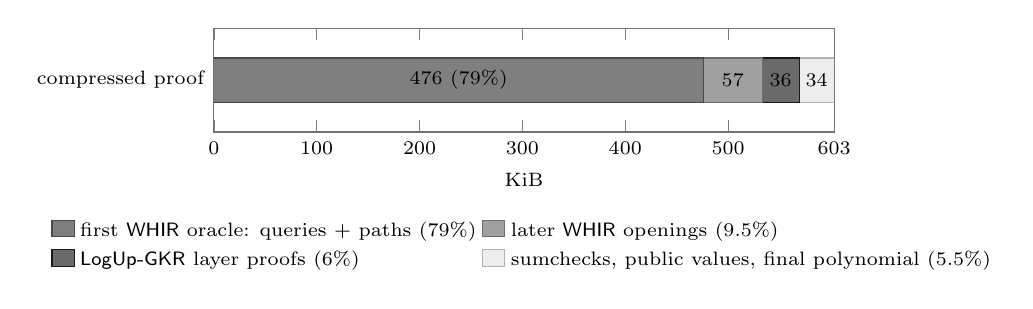
\begin{tikzpicture}
\begin{axis}[
  xbar stacked, xmin=0, xmax=603, width=0.78\textwidth, height=2.9cm, bar width=16pt,
  ymin=-0.5, ymax=0.5, ytick={0}, yticklabels={compressed proof},
  xlabel={KiB}, xtick={0,100,200,300,400,500,603},
  axis line style={black!55},
  legend style={font=\scriptsize, at={(0.5,-0.75)}, anchor=north, legend columns=2, cells={anchor=west}, draw=none},
  tick label style={font=\scriptsize}, label style={font=\scriptsize},
  nodes near coords, every node near coord/.append style={font=\scriptsize, /pgf/number format/fixed, /pgf/number format/precision=0},
  point meta=explicit symbolic,
]
\addplot[fill=zirenblue!72, draw=zirenblue!95!black] coordinates {(476,0) [476 (79\%)]}; \addlegendentry{first \WHIR{} oracle: queries + paths (79\%)}
\addplot[fill=zirenteal!68, draw=zirenteal!95!black] coordinates {(57,0) [57]}; \addlegendentry{later \WHIR{} openings (9.5\%)}
\addplot[fill=zirenorange!65, draw=zirenorange!95!black] coordinates {(36,0) [36]}; \addlegendentry{\LogUp{} layer proofs (6\%)}
\addplot[fill=zirenslate!18, draw=zirenslate!75] coordinates {(34,0) [34]}; \addlegendentry{sumchecks, public values, final polynomial (5.5\%)}
\end{axis}
\end{tikzpicture}
}
\caption{In the instrumented pre-correction proof (617\,618 bytes), openings of the first \WHIR{} oracle account for 79\% because each query authenticates one coset row of every stripe. The retained census describes an earlier configuration and does not reproduce this exact file.}
\label{fig:proofsize}
\end{figure}

\section{Recursion}
\label{sec:recursion}

This section describes the block's outward interface: what leaves it is the root of the tree built here, the compressed proof of Table~\ref{tab:ports}, and what binds that proof to the advertised machine is the verifying-key allowlist of the last paragraph. Shard proofs are aggregated by a recursion machine: a small register VM over the same field whose programs are compiled from a description of the verifier, executed to a trace, and proved by the same unit/\LogUp{}/zerocheck/Jagged/\WHIR{} pipeline. Its units are the arithmetic of $\F$ and $\EF$, memory, the $\Poseidon{}$ permutation, a select gate and a batched folding gate for the FRI-style query checks.

\paragraph{Leaves.} A \emph{leaf} program verifies one core shard proof in four phases mirroring the host verifier: the transcript prologue (public values, commitment, unit dimensions), the \LogUp{} layer replay, the zerocheck replay including the constraint evaluation of every unit present, and the jagged opening with its branching-program closing identity followed by the \WHIR{} verifier. Because the jagged verifier depends only on the shard's log-area and the constraint evaluation only on the unit set, the number of distinct leaf programs is small; on the single-GPU deployment consecutive shards of the same class reuse a device-resident proving key. Adjacent shards' leaves are \emph{fused} into one node where the shard shapes allow, and leaves are proved on the same GPU concurrently with core shards, so that the GPU's time is shared between the two stages rather than serialised.

Figure~\ref{fig:recursion} shows the tree, what each node checks on its
children and what the root closes.

\begin{figure}[t]
\centering
\resizebox{0.96\textwidth}{!}{% The compose relation: what each node reads, what it checks, what the root closes.
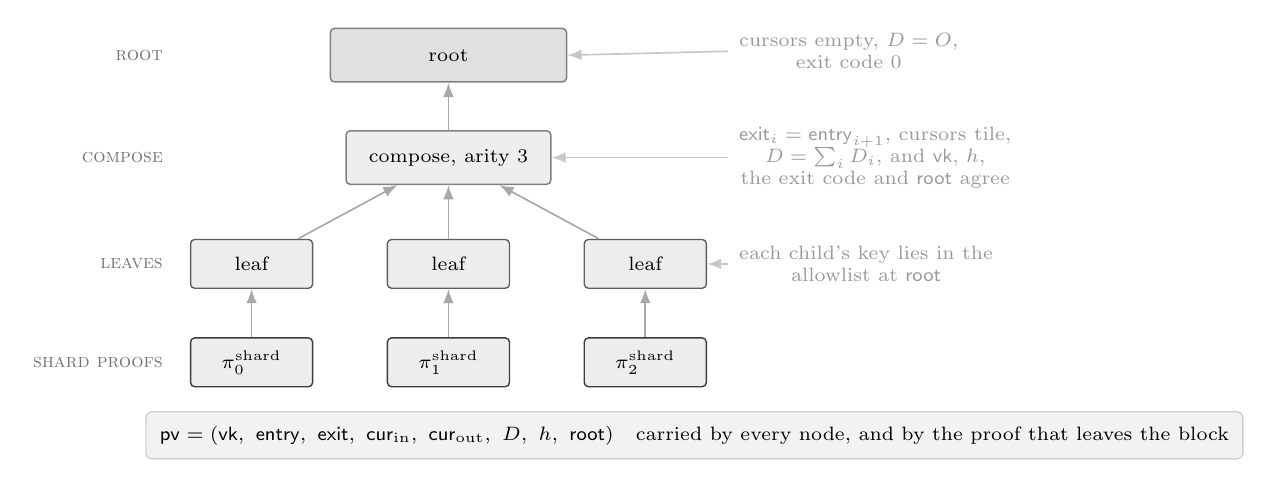
\begin{tikzpicture}[
  font=\small,
  shard/.style={rectangle, rounded corners=1.5pt, draw=zirenorange!85, fill=zirenorange!8,
                minimum width=1.55cm, minimum height=0.62cm, align=center, font=\scriptsize,
                line width=0.5pt},
  leaf/.style={rectangle, rounded corners=1.5pt, draw=zirenblue!90, fill=zirenblue!10,
               minimum width=1.55cm, minimum height=0.62cm, align=center, font=\scriptsize,
               line width=0.5pt},
  comp/.style={rectangle, rounded corners=1.5pt, draw=zirenteal!90, fill=zirenteal!12,
               minimum width=2.6cm, minimum height=0.68cm, align=center, font=\scriptsize,
               line width=0.55pt},
  root/.style={comp, draw=zirenteal!90, fill=zirenteal!22, minimum width=3.0cm},
  a/.style={-{Latex[length=1.8mm]}, line width=0.6pt, zirenslate!85},
  cond/.style={font=\scriptsize, zirenslate, align=center, inner sep=1pt},
  side/.style={rectangle, rounded corners=2pt, draw=zirenslate!45, fill=zirenlight,
               align=left, font=\scriptsize, inner sep=5pt, line width=0.5pt},
  band/.style={font=\scriptsize\scshape, black!55, anchor=east, inner sep=2pt},
]

% ---- shard proofs, each with the public values it publishes
\foreach \k/\x in {0/0, 1/2.5, 2/5.0} {
  \node[shard] (s\k) at (\x,0) {$\pi^{\mathrm{shard}}_\k$};
}
\node[band] at (-1.05,0) {shard proofs};

% ---- one leaf per shard proof
\foreach \k/\x in {0/0, 1/2.5, 2/5.0} {
  \node[leaf] (l\k) at (\x,1.25) {leaf};
  \draw[a] (s\k) -- (l\k);
}
\node[band] at (-1.05,1.25) {leaves};

% ---- one compose node of arity three
\node[comp] (c) at (2.5,2.6) {compose, arity $3$};
\foreach \k in {0,1,2} { \draw[a] (l\k) -- (c); }
\node[band] at (-1.05,2.6) {compose};

\node[root] (r) at (2.5,3.9) {root};
\draw[a] (c) -- (r);
\node[band] at (-1.05,3.9) {root};

% ---- what the compose node checks on its children
\node[cond, anchor=west] at (6.15,1.25)
  {each child's key lies in the\\allowlist at $\mathsf{root}$};
\draw[a, zirenslate!55] (6.05,1.25) -- (l2.east);

\node[cond, anchor=west] at (6.15,2.6)
  {$\mathsf{exit}_i=\mathsf{entry}_{i+1}$, cursors tile,\\
   $D=\sum_i D_i$, and $\mathsf{vk}$, $h$,\\
   the exit code and $\mathsf{root}$ agree};
\draw[a, zirenslate!55] (6.05,2.6) -- (c.east);

\node[cond, anchor=west] at (6.15,3.95)
  {cursors empty, $D=O$,\\exit code $0$};
\draw[a, zirenslate!55] (6.05,3.95) -- (r.east);

% ---- the tuple every node carries
\node[side, anchor=north west] at (-1.35,-0.62)
  {$\mathsf{pv}=(\mathsf{vk},\ \mathsf{entry},\ \mathsf{exit},\
    \mathsf{cur}_{\mathrm{in}},\ \mathsf{cur}_{\mathrm{out}},\ D,\ h,\ \mathsf{root})$\quad
   carried by every node, and by the proof that leaves the block};
\end{tikzpicture}
}
\caption{Every node of the tree carries the same public-value tuple, so a
compose node checks its children by comparing tuples: the ranges must be
adjacent, the cursors must tile and the digests must accumulate, while the
verifying key, the output digest, the exit code and the allowlist root must
agree. The root is where the memory argument and the cross-shard digest close,
and where the exit code is required to be the one the relation admits.}
\label{fig:recursion}
\end{figure}

\paragraph{The compose relation.} Write a node's public values as
\[
  \mathsf{pv} = (\mathsf{vk}, \mathsf{entry}, \mathsf{exit}, \mathsf{cur}_{\mathrm{in}}, \mathsf{cur}_{\mathrm{out}}, D, h, \mathsf{code}, \mathsf{root}),
\]
the verifying key of the guest, the entry and exit machine states, the
memory-address cursors the node opens and closes with, the accumulated
cross-shard digest, the digest of committed output, the exit code, and the
root of the allowlist of admissible recursion keys. For a machine with a delay slot the entry and exit states are
\emph{pairs} $(\mathsf{pc}, \mathsf{pc}_{\mathrm{next}})$, because a row's successor is
data; adjacency therefore has to pin both components, and a defect in which only
the first was pinned across shards is recorded in Table~\ref{tab:defects}.
A compose node of arity $k$ proves the
relation $\mathcal R_{\mathrm{comp}}(\mathsf{pv}; \pi_0,\dots,\pi_{k-1})$,
which holds when each $\pi_i$ verifies against a key that the allowlist at
$\mathsf{root}$ contains, the children agree on $\mathsf{vk}$, $h$ and $\mathsf{code}$, their
$\mathsf{root}_i$ all equal the $\mathsf{root}$ that membership is checked
against and that the node publishes, their ranges are adjacent in the sense that
$\mathsf{exit}_i = \mathsf{entry}_{i+1}$ and
$\mathsf{cur}_{\mathrm{out},i} = \mathsf{cur}_{\mathrm{in},i+1}$, and the
output satisfies $\mathsf{entry} = \mathsf{entry}_0$,
$\mathsf{exit} = \mathsf{exit}_{k-1}$,
$\mathsf{cur}_{\mathrm{in}} = \mathsf{cur}_{\mathrm{in},0}$,
$\mathsf{cur}_{\mathrm{out}} = \mathsf{cur}_{\mathrm{out},k-1}$ and
$D = \sum_i D_i$. 

\paragraph{Leaves and the root.} A leaf node proves the corresponding relation for a single child, with one
difference that matters: its child is a core shard proof, which verifies
against the guest's $\mathsf{vk}$ rather than against a key of the allowlist.
It is the leaf's own key that the allowlist must contain, and its parent is
what checks that. The root additionally requires
$\mathsf{cur}_{\mathrm{in}}$ and $\mathsf{cur}_{\mathrm{out}}$ to be the
empty cursors, $D$ to be the identity and the exit code to be zero, which is
what closes the memory argument and the cross-shard digest over the whole
execution and admits only the halts the relation of
Section~\ref{sec:statement} accepts.
Algorithm~\ref{alg:compose} states the same checks as the procedure a compose
node runs, with the root's extra conditions on the last line.

\begin{algorithm}[t]
\caption{The compose node of arity $k$, and what the root additionally
requires. Line~2 is the binding of \S\ref{sec:recursion}: without it the node
would verify \emph{some} proof rather than a proof of this machine.}
\label{alg:compose}
\DontPrintSemicolon
\KwIn{child proofs $\pi_0,\dots,\pi_{k-1}$ with public values
      $\mathsf{pv}_0,\dots,\mathsf{pv}_{k-1}$ and membership paths
      $\mathsf{path}_0,\dots,\mathsf{path}_{k-1}$; a claimed allowlist root $\mathsf{root}$}
\KwOut{the node's public values $\mathsf{pv}$, or $\bot$}
\For{$i \gets 0$ \KwTo $k-1$}{
  \lIf{$\neg\,\mathsf{MerkleVerify}(\mathsf{root}, \mathsf{vk}_i, \mathsf{path}_i)$}{\Return $\bot$
    \tcp*[f]{the child's key is admissible}}
  \lIf{$\neg\,\mathsf{Verify}(\mathsf{vk}_i, \mathsf{pv}_i, \pi_i)$}{\Return $\bot$}
}
\lIf{$\exists\, i:\ \mathsf{root}_i \neq \mathsf{root}$}{\Return $\bot$
    \tcp*[f]{children agree with the root they were checked against}}
\lIf{$\mathsf{vk}_i$, $h_i$, $\mathsf{code}_i$ not all equal over $i$}{\Return $\bot$}
\For{$i \gets 0$ \KwTo $k-2$}{
  \lIf{$\mathsf{exit}_i \neq \mathsf{entry}_{i+1}$}{\Return $\bot$
    \tcp*[f]{ranges adjacent}}
  \lIf{$\mathsf{cur}_{\mathrm{out},i} \neq \mathsf{cur}_{\mathrm{in},i+1}$}{\Return $\bot$
    \tcp*[f]{cursors tile}}
}
$D \gets \sum_{i} D_i$ \tcp*{digests accumulate}
$\mathsf{pv} \gets (\mathsf{vk},\ \mathsf{entry}_0,\ \mathsf{exit}_{k-1},\
  \mathsf{cur}_{\mathrm{in},0},\ \mathsf{cur}_{\mathrm{out},k-1},\ D,\ h,\ \mathsf{root})$\;
\If{this node is the root}{
  \lIf{$\mathsf{cur}_{\mathrm{in}}, \mathsf{cur}_{\mathrm{out}}$ non-empty
       $\lor\ D \neq O \lor \mathsf{code} \neq 0$}{\Return $\bot$}
}
\Return $\mathsf{pv}$\;
\end{algorithm}
 The tree merges contiguous shard \emph{ranges} as soon as they are complete rather than level by level, which shortens the tail after the last core shard from four serial composes to two; that tail is one of the two components of the gap to linear scaling in \S\ref{sec:perf-after}. Because a range is reduced the moment it is complete, the tree climbs on the workers that are still proving core shards, and on the deployed configuration the root is finished before the last shard's proof is collected. A leaf is never itself the root: an execution of a single shard closes through a compose of arity one, which costs one more node and keeps the leaf programs to the open classes that the enumeration below covers. Arity is capped at three by the recursion units' height budget; arity four was built and measured, and it was neutral (41 nodes replaced by 27, $-0.7\%$ of wall time, an unchanged tail), so it does not pay for the key regeneration it would force.

\paragraph{Shrink and wrap.} The root proof is \emph{shrunk} to a fixed shape and then \emph{wrapped} on the outer ring: a jagged proof whose dense polynomial is committed with a FRI-style BaseFold instantiation over the same field but with a 254-bit hash, folding one variable per round under query grinding down to a small final polynomial. The artifact report estimates 534\,KiB expected and 963\,KiB worst case for the checked-in 16-bit-lookup-grinding schedule; these are configuration estimates rather than measurements of the zero-grinding baseline in Section~\ref{sec:performance}. The wrap proof is what a Groth16 verifier on BN254, generated with \texttt{gnark}~\citep{gnark}, consumes when an on-chain proof is required. For the block-proving service and throughout this paper, the compressed inner-ring proof itself is the published artefact.

\paragraph{Verifying-key binding.} Every recursion program has a verifying key. The statement of Section~\ref{sec:statement} is only about the advertised machine if the verifier can tell that the leaf it is looking at verified a \emph{core} proof of that machine and that every compose node ran the compose program: the compose program therefore checks that its children's keys belong to a Merkle allowlist, and the root of that allowlist is checked against the one compiled into the verifier. Which verifier matters: inside the tree the root is a witness the prover supplies, so the in-circuit checks establish only that every child's key lies in a tree with \emph{that} root. The root is therefore carried out of the tree as a public value of the compressed proof and, for the wrapped proof, as a public input of the wrap circuit, where the on-chain verifier supplies the published root rather than accepting one from its caller. It was not always so, and the gap is recorded in Table~\ref{tab:defects}. The recursion machine is outside the extraction of Section~\ref{sec:verification}, so Theorem~\ref{thm:composition} takes this binding as a hypothesis. It is part of the protocol: a proof produced by a prover configured to skip the in-circuit check has a different compose key and is rejected (Section~\ref{sec:verification} reports finding this configuration in the block-proving service). The allowlist is regenerated whenever the arithmetisation changes, and it is now enumerated for the leaf programs as well as the compose ones, which is what makes it a statement about the machine rather than about one guest.

\paragraph{Enumerating the leaf keys.} A leaf program is determined by the geometry of the shard proof it verifies, and Section~\ref{sec:pcs-geometry} quantises that geometry: the committed area of each round is a bucket rather than an exact cell count, and the padding-column count is a function of the bucket alone. What remains is the shard's chip set, which is one of the machine's fixed clusters, and the two bucket indices. Enumerating those triples and building one program per class gives, without running a single guest, every leaf key a prover can produce for a shard whose chip set is one of those clusters: about $6.4 \cdot 10^3$ keys for the deployed machine. The scope of that statement is the cluster list. A \emph{cluster} is one of the chip-set combinations the machine's shape configuration declares, curated from the combinations that arise in the workloads it is built for, not an exhaustive partition of the chip powerset. So the enumeration is exhaustive given the list, and the allowlist covers an arbitrary guest only to the extent that the list does; \S\ref{sec:scope} says the same thing from the other side. What that buys is bounded on the right axis: a shard whose chip set falls outside the list produces a key the allowlist does not contain, and a verifier that requires membership refuses it. The failure is of completeness, not of soundness, and it is loud. 

\paragraph{Why not sample the keys.} Before this the leaf keys were \emph{sampled}: a corpus of executions was proved and the keys they happened to produce were collected, which covers the workload that was sampled and leaves the next shard shape one uncollected key away from a refusal. A verifier configured to require membership on a sampled allowlist did exactly that in the block-proving service, which is how the omission was found. The enumeration is checked against the sampled corpus, class by class, and against the programs the classes generate.
Algorithm~\ref{alg:enum} states the procedure; every quantity it ranges over
is fixed by the machine and the committed geometry, so it terminates without
consulting any execution.

\begin{algorithm}[t]
\caption{Enumerating the admissible leaf keys. The loop bounds come from the
machine's unit clusters and from the bucket rule of \S\ref{sec:pcs-geometry};
no guest is executed. For the deployed machine it returns about
$6.4 \cdot 10^{3}$ keys.}
\label{alg:enum}
\DontPrintSemicolon
\KwIn{unit clusters $\mathcal{C}$; bucket sets $\mathcal{B}_{\mathrm{prep}}$,
      $\mathcal{B}_{\mathrm{main}}$; padding rule $\mathsf{pad}(\cdot)$}
\KwOut{the allowlist root $\mathsf{root}$}
$K \gets \emptyset$\;
\ForEach{cluster $c \in \mathcal{C}$}{
  \ForEach{$b_{\mathrm{p}} \in \mathcal{B}_{\mathrm{prep}}$,
           $b_{\mathrm{m}} \in \mathcal{B}_{\mathrm{main}}$}{
    $n \gets \mathsf{pad}(b_{\mathrm{m}})$ \tcp*{a function of the bucket, not of the real count}
    \ForEach{$\mathit{first} \in \{\mathsf{true}, \mathsf{false}\}$}{
      $\sigma \gets (c,\ \mathit{first},\ b_{\mathrm{p}},\ b_{\mathrm{m}},\ n)$
        \tcp*{the shape a leaf can be asked to verify}
      $K \gets K \cup \{\,\mathsf{vk}(\mathsf{CompileLeaf}(\sigma))\,\}$\;
    }
  }
}
\Return $\mathsf{MerkleRoot}(K)$\;
\end{algorithm}

\section{The verification flow and its findings}
\label{sec:verification}

The soundness argument of Sections~\ref{sec:air}--\ref{sec:iopp} establishes that an accepting proof implies the existence of a trace satisfying every constraint. Two further questions decide whether that trace is an execution of the advertised machine: does the executor implement the ISA, and does each constrained unit admit exactly one output behaviour for a fixed input? We address both with a specification-derived conformance suite against an independent reference, an executable formal model, and per-unit uniqueness theorems. This section reports the verification artifacts of \S\ref{sec:ipcore-collateral}: the suites and their reference results, the formal model and its two checks, the extracted theorems with the tactic that discharges them and the list of those still open, and the defects register of Table~\ref{tab:defects}. A deployer reads them to decide what has been established for a release and what remains conditional.

\subsection{ISA conformance}
\label{sec:verification-isa}

\paragraph{Vectors from the specification.} The MIPS32 architecture manual's encoding tables were transcribed into a machine-readable table of 77 instructions (all integer, shift, branch, jump, load/store, bit-manipulation and conditional-move forms the guest supports), reproduced with the unit that proves each one in Appendix~\ref{sec:app-isa}. For each instruction a generator emits ten programs with pseudo-random operands, boundary values and the delay-slot placements the instruction admits, assembled with \texttt{llvm-mc}; the reference is the Unicorn/QEMU MIPS32 emulator~\citep{unicorn}, which shares no code with \Ziren{}'s own, and each vector compares the general registers, \texttt{HI}/\texttt{LO} and the touched memory after execution. All 770 vectors agree, on both the interpreter and the JIT.

\paragraph{Shared instruction suites.} The generated vectors cover the encoding space broadly but shallowly. A second collection contains fifteen hand-written suites, 144 cases in all, for instructions with difficult MIPS32 semantics: signed and unsigned division, multiply-accumulate pairs, bit-field and byte-order instructions, rotates, and count-leading-one and count-leading-zero instructions. One crate supplies case data to both the emulator and the prover tests, so every case is executed and proved against the same result. The generated vectors are shared in the same way. A regression in only the emulator or prover therefore appears as a disagreement rather than two tests drifting together.

\paragraph{The Cannon suite.} The third suite is independent of us. Optimism's Cannon ships a suite of hand-written MIPS test programs~\citep{cannon}, written by the fault-proof project whose ISA semantics a hybrid deployment must match (\S\ref{sec:ipcore-integration}); they exercise the machine against another team's reading of the architecture manual rather than against our own generator or our own regressions. A harness byte-swaps them to little-endian and adapts the halt convention; the 49 programs applicable to a little-endian guest all pass.

\paragraph{From vectors to proofs.} 224 of the generated programs and 48 of the 49 Cannon programs were also proved end to end and verified. The single exception halts with a non-zero exit code, which the emulator accepts and the arithmetisation does not admit as a valid execution to prove. On everything else the arithmetisation accepts every behaviour the reference exhibits; the next subsection is the converse direction.

\paragraph{Executable formal model.} A \Lean{} model of the ISA was written independently of \Ziren{}'s emulator: a decoder transcribed from the encoding tables, an interpreter with the delay-slot program-counter pair and little-endian byte memory, and an ALU. Two checks connect it to the implementation, both discharged by \texttt{native\_decide}: the decoder agrees with the emulator's decoder on all 2\,275 distinct instruction words appearing in the vectors, and the model reproduces the reference emulator's results on all 770 vectors. \Ziren{}'s two emulator implementations are additionally run twice on every vector with a digest of the emitted event records; the digests agree between runs and between the interpreter and the JIT, and this is evidence of reproducibility rather than a proof of determinism.

\subsection{Determinism of the units}
\label{sec:verification-det}

\paragraph{What is proved.} For a unit $U$ with constraint system $C_U$ over a row $w$ of columns, and with \emph{inputs} $I_U(w)$ (the values the row receives on its buses: the fetched instruction, the register and memory values read, the incoming state) and \emph{outputs} $O_U(w)$ (the values it sends: the register and memory values written, the outgoing state), determinism is the statement
\[
  \forall w, w'.\; C_U(w) \wedge C_U(w') \wedge I_U(w) = I_U(w') \;\Rightarrow\; O_U(w) = O_U(w').
\]
The statement is Definition~\ref{def:det}, with byte-table lookups lowered to range constraints or to calls of an abstract deterministic table.

Theorem~\ref{thm:unique} is what makes a satisfying trace unique given the determinism of every unit. The theorems below are its premises, machine-checked for the units the automation closes and stated with an explicit gap for the rest.

\paragraph{Extraction.} The theorems are not written by hand. The same Rust constraint description that the prover evaluates and the verifier checks is evaluated once with symbolic columns, the resulting polynomial constraints, range facts and bus interactions are lowered to a first-order statement, and a generator emits one \Lean{} file per unit: a record type for the row, the constraints as a conjunction, the input and output projections with their provenance, and the theorem above. Selector-specialised units (one theorem per opcode selector) and an \emph{is\_real}~$=1$ specialisation keep each statement about real rows of one opcode. The extraction covers every unit of the core machine catalogued in Appendix~\ref{sec:app-units}: \ndettotal{} determinism theorems.

\paragraph{Proof automation.} A theorem is closed by a tactic that lifts the statement from $\F$ to the integers: every column is replaced by an integer with the bound its range fact gives (a byte, a 16-bit limb, a bit, or $[0, p)$ when unconstrained), every field equation becomes an exact integer equation once its slack is shown to vanish under those bounds, and the remaining goal is linear arithmetic over bounded integers, decided by \Lean{}'s \texttt{omega}. Between the lifting and the decision the tactic runs the propagation loop of Picus inside the proof assistant: it proves corresponding columns of $w$ and $w'$ equal one pair at a time, substitutes, resolves selector bits to constants, and case-splits only on selector bits already known to agree. The automation runs with a fixed wall-clock budget per theorem. 

\paragraph{Coverage.} At the time of writing \ndetproved{} of the \ndettotal{} theorems are closed (Figure~\ref{fig:verification}, by unit family). \ndetopen{} were attempted and remain open: integer units whose constraints multiply by $2^{24}$ or $2^{32}$ and are only meaningful modulo $p$ (multiply, the conditional moves, the memory-argument units), which the integer lifting does not model, or whose selector case structure exceeds the split budget. \ndetskipped{} are not attempted by the generator: \ndetskipacc{} are accelerator units above the size threshold (the same theorem at 1\,000--5\,600 conjuncts), and \ndetskipcase{} are units whose constraints contain comparison case-splits from the byte-table summaries, which the current tactic does not handle. \ndetpending{} had not finished their attempt when the numbers were taken. The syscall unit, which was under-determined as first extracted (next paragraph), closes after the bus change; the count above is therefore for the constraint system with that change applied. Two units separate it from the system measured in Section~\ref{sec:performance}: that one, and the hash unit, whose round schedule was corrected afterwards (Table~\ref{tab:defects}). All theorem statements compile; open ones carry an explicit \texttt{sorry} and are listed in the artifact.

\begin{figure}[t]
\centering
% Status of the extracted determinism theorems, per chip family.
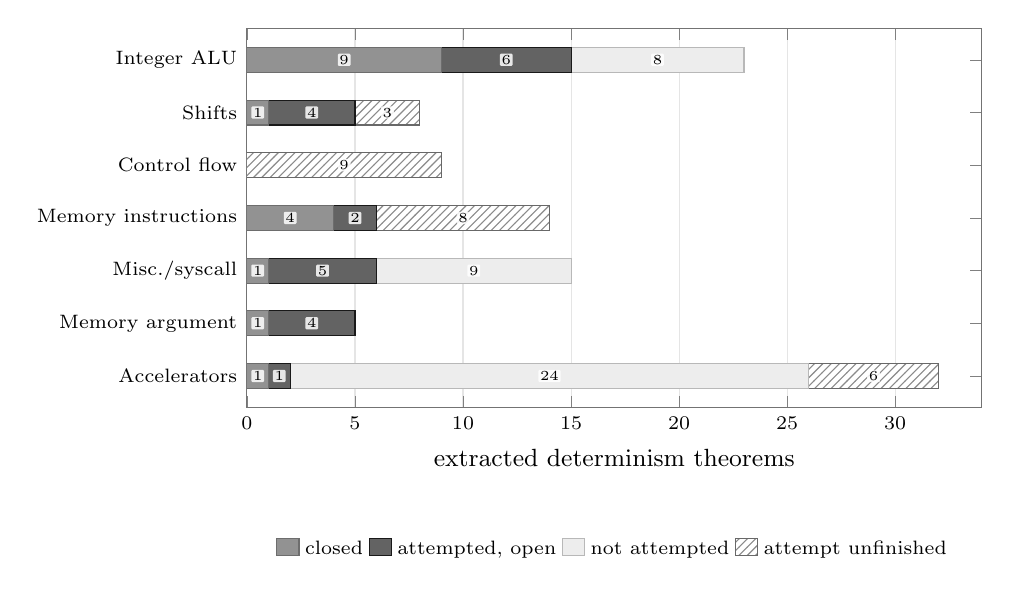
\begin{tikzpicture}
\begin{axis}[
  xbar stacked, xmin=0, xmax=34, width=0.9\textwidth, height=6.4cm, bar width=9pt,
  symbolic y coords={Accelerators,Memory argument,Misc./syscall,Memory instructions,Control flow,Shifts,Integer ALU},
  ytick=data, y dir=normal,
  xlabel={extracted determinism theorems},
  xmajorgrids, grid style={black!10}, axis line style={black!55},
  legend style={font=\scriptsize, at={(0.5,-0.32)}, anchor=north, legend columns=4, draw=none},
  tick label style={font=\scriptsize}, label style={font=\small},
  nodes near coords,
  % the counts sit on hatched segments, so give each one an opaque backing
  every node near coord/.append style={font=\tiny, fill=white, fill opacity=0.85,
    text opacity=1, inner sep=0.6pt, rounded corners=0.4pt},
  point meta=explicit, nodes near coords style={/pgf/number format/fixed},
]
\addplot[fill=zirenteal!78, draw=zirenteal!95!black] coordinates {(9,Integer ALU) [9] (1,Shifts) [1] (0,Control flow) [] (4,Memory instructions) [4] (1,Misc./syscall) [1] (1,Memory argument) [1] (1,Accelerators) [1]}; \addlegendentry{closed}
\addplot[fill=zirenorange!68, draw=zirenorange!95!black] coordinates {(6,Integer ALU) [6] (4,Shifts) [4] (0,Control flow) [] (2,Memory instructions) [2] (5,Misc./syscall) [5] (4,Memory argument) [4] (1,Accelerators) [1]}; \addlegendentry{attempted, open}
\addplot[fill=zirenslate!18, draw=zirenslate!70] coordinates {(8,Integer ALU) [8] (0,Shifts) [] (0,Control flow) [] (0,Memory instructions) [] (9,Misc./syscall) [9] (0,Memory argument) [] (24,Accelerators) [24]}; \addlegendentry{not attempted}
\addplot[fill=white, draw=zirenblue!85, postaction={pattern=north east lines, pattern color=zirenblue!65}] coordinates {(0,Integer ALU) [] (3,Shifts) [3] (9,Control flow) [9] (8,Memory instructions) [8] (0,Misc./syscall) [] (0,Memory argument) [] (6,Accelerators) [6]}; \addlegendentry{attempt unfinished}
\end{axis}
\end{tikzpicture}

\caption{The current artifact closes \ndetproved{} of \ndettotal{} extracted unit and opcode-selector determinism statements. The remaining statements are open, skipped because of accelerator size or comparison case splits, or unfinished under the fixed automation budget.}
\label{fig:verification}
\end{figure}

\subsection{A negative control for the height claims}
\label{sec:verification-forgery}

The suites above test that the machine accepts what it should. A verification
flow also needs the opposite evidence: that the argument \emph{rejects} a
trace whose declared shape is a lie. This matters here because the shape is
not incidental. The verifying key is a function of the chip set
(\S\ref{sec:recursion}), the committed geometry is quantised from the declared
heights (\S\ref{sec:pcs-geometry}), and the enumeration of admissible leaf
keys rests on both. If a prover could declare a shape it did not execute, the
enumeration would be a statement about nothing.

A harness therefore proves real shard proofs and then tampers with the claimed
heights before verification, in eighteen cases across two guests, an
arithmetic one and a hash-heavy one. The forgeries are over- and under-claims
of a unit's height, lies about which units are active, tampering with the
column count and tampering with the row count, each injected at the stage that
would carry it: the degree mask alone, the Fiat--Shamir prologue alone, and
both together. Every case is rejected, and the interest is in which check
rejects it, because no single mechanism covers the space.

\begin{itemize}
  \item Height and activity lies that reach the degree mask are caught by the
  \LogUp{} last-layer reconstruction, as a numerator or denominator mismatch.
  \item Lies confined to the transcript are caught by the grinding witness,
  because the Fiat--Shamir prologue observes the declared heights, so a changed
  height invalidates the proof of work.
  \item A tampered column count is caught by the jagged verifier, and a
  tampered row count by the preprocessed round, which takes the row count from
  the verifying key rather than from the prover.
\end{itemize}

One case in the harness is a control on the control: a degree-only over-claim
that an earlier configuration allowed to survive, because the reconstruction
could be disabled. That configuration no longer exists, the anchor is
unconditional, and the case now expects rejection. A negative control whose
negative case cannot fail is not a control, which is why it is reported here
rather than removed.

\subsection{Findings}
\label{sec:verification-findings}

The flow surfaced nine defects, and their discovery methods distinguish three classes. Three determinism-theorem findings are under-constraints, where the constraints permit more than one value. Three end-to-end proving findings are integration mistakes between components that use different conventions. Three line-by-line comparison findings are omitted checks, a class that neither honest tests nor local determinism statements can detect.

That distinction is worth stating plainly, because it bounds what the first two techniques can establish. A determinism theorem asks whether the constraints present admit two behaviours; it is silent about a constraint that was never written, since its absence makes no theorem false. Testing is silent for the same reason: an omitted check breaks nothing that an honest execution does, so no test fails. The completeness flag left unpinned at the terminal stages is the sharpest example. Every honest proof sets it, so every test passes and every extracted theorem holds; only a reader asking what enforces it finds that nothing does. Differential reading against an independent implementation of the same protocol is the cheapest way we know to find that class, and it is the reason we report it as a third technique rather than as incidental review.

Appendix~\ref{sec:app-defects} tabulates all nine. One is described in detail here, because it is the one the extracted theorems found unaided and it shows what such a theorem does and does not say.



\paragraph{Syscall argument half-words.} The syscall unit receives two reduced 32-bit arguments from the instruction that raised the syscall and witnesses each of them, written $a \in \F$ here, as two 16-bit half-words $a_{\mathrm{lo}}, a_{\mathrm{hi}}$ constrained by $a_{\mathrm{lo}} + 2^{16} a_{\mathrm{hi}} = a$ in $\F$ and two 16-bit range checks. Because $2^{32} > p$, this does not determine the half-words: for every $a \in \F$ both the decomposition of $a$ and that of $a + p$ satisfy the constraints, since $2p < 2^{32}$. The extracted theorem for the unit is false and the automation reports exactly these four half-word columns as open. Whether the ambiguity is exploitable depends on the consumer: an accelerator that re-reduces the half-words modulo $p$ sees the same field element either way, while one that uses them as an exact 32-bit pointer does not. The finding is a specification gap between the two sides of the syscall bus. The remedy, applied after the finding, is to carry the half-words rather than the reduced sum on the bus, together with the unit's Linux selector; with that change the unit's determinism theorem closes in under a minute. The change alters the constraints of two units and therefore the verifying keys, so it is staged with the next key-changing release rather than deployed alone.

\section{Evaluation}
\label{sec:performance}

This section reports two metrics in one deliberately narrow environment. \emph{Emulator efficiency} is the rate at which the software emulator turns a guest program into the prover's input record, together with the associated host memory and processor time (\S\ref{sec:perf-emu}). \emph{Prover efficiency} is the rate at which that record becomes a proof, together with its trace area and proof size (\S\ref{sec:perf-prover}). The environment uses one workload, one GPU model, one host and interleaved repetitions on the same input so that differences between configurations are attributable.

\paragraph{Measurement status.} Every timing and proof-size result in this section was collected before the Poseidon2 schedule was corrected from 8 full plus 13 partial rounds to 8 full plus 20 partial rounds. The correction affects commitments, Fiat--Shamir and recursion. The measurements therefore compare engineering changes within the pre-correction implementation; they do not report the absolute performance or proof artifact of the corrected release. Section~\ref{sec:perf-threats} records this and the workload limitations.

\paragraph{Deployment.} The system runs continuously in production rather
than only in this evaluation: one deployment proves Ethereum mainnet blocks as
they arrive on commodity GPUs, and others, the GOAT Network among them, prove
different programs on the same prover. What follows measures the block
workload, because it is the one with a public reference point; no claim here
depends on the others.

\subsection{Experimental setup}
\label{sec:perf-setup}

\paragraph{Workload.} The workload is Ethereum mainnet block 25\,907\,955 executed by a MIPS32 build of the \texttt{reth} execution client with a witness trie represented as an arena. We use it because this class of system is publicly compared on block proving and because its instruction mix represents hash-intensive computation: the guest hashes trie nodes, recomputes a Merkle root over state it does not hold and verifies signatures. It is not a workload-diverse benchmark, and \S\ref{sec:perf-threats} bounds the conclusions accordingly. A word-wise \texttt{memcmp}, zero-copy Keccak wrapper and arena representation of the witness trie reduce the block from 379 to 288 million cycles. Every single-GPU prover measurement uses that cached record, so all runs execute the same instruction stream. The multi-GPU measurements of \S\ref{sec:perf-after} use three further blocks of 420, 530 and 912\,M cycles.

\paragraph{Hardware.} One NVIDIA RTX~5090 (32\,GB) in a host that holds eight of them, with one AMD EPYC 9355 processor and 925\,GB of memory; the multi-GPU measurements use four of the eight (driver 570.153.02, CUDA 12.8, Ubuntu 22.04). The prover is pinned to one GPU.

\paragraph{Metrics.} \emph{Wall-clock time} is the end-to-end proving-process time from reading the cached input to writing the compressed proof. It includes host verification of every shard proof and the compressed proof, which accounts for 2--3\,s and would be omitted by a production service. \emph{Emulation rate} is guest cycles divided by the emulator's wall-clock time. \emph{Proving throughput} is guest cycles divided by the whole proving process's wall-clock time. The latter includes the former, so the rates are not directly comparable; neither is a clock frequency. \emph{Trace area} is the sum over units of rows $\times$ columns, in cells, from the emulator's shard-close census and the unit widths. Table~\ref{tab:chips}, in Appendix~\ref{sec:app-units}, gives the widths of the release this paper describes, while Table~\ref{tab:census} uses those of the evaluated revision, which precede the changes of \S\ref{sec:perf-changes}; the appendix says where the two differ. \emph{Proof size} is the byte length of the serialised compressed proof. A ten-shard \texttt{nsys} sample attributes GPU kernel time to kernel groups.

\paragraph{Software revision.} The implementation described throughout the paper is v2.0.0, whose \Poseidon{} permutation uses 8 full and 20 partial rounds. The measurements below were taken on earlier revisions of that branch, before the round correction, each row of Table~\ref{tab:levers}, in Appendix~\ref{sec:app-levers}, adding its change to the row above it. The GPU backend is a separate CUDA implementation of the same protocol. No raw per-run timing bundle is retained (\S\ref{sec:perf-threats}).

\paragraph{Protocol.} Each pair of configurations is measured in interleaved A/B/B/A order on the same GPU and the same input, and medians are reported; the spread over three repetitions was within $\pm 1$\,s of the median for every row of Table~\ref{tab:levers} and within $\pm 0.8$\,s for Table~\ref{tab:cards}. The GPU under measurement was otherwise idle; a second, unrelated proving process ran on another GPU of the same host, so the host processor was not idle.

\subsection{Emulator efficiency}
\label{sec:perf-emu}
\label{sec:perf-host}

The emulator is the block's front end: everything the prover consumes passes through it, and on a host driving several GPUs its cost, not the accelerator's, is what binds (below). Its two implementations differ by an order of magnitude in rate. On the block of \S\ref{sec:perf-setup} the just-in-time compiler emulates the guest at roughly 130\,MHz, while the interpreter runs at 5--20\,MHz depending on whether it is recording events. That rate is the compiled emulator alone. A coordinator's producer also writes each shard's descriptor, and the last row of Table~\ref{tab:host}, in Appendix~\ref{sec:executor}, is that whole job at 6.1\,s for a 420\,M-cycle block, some 69\,MHz. They produce the same records on the differential-test corpus (Section~\ref{sec:isa}), so the measured rate difference does not change those tested witnesses. The compiled emulator is therefore some twenty times faster than proving and the interpreter roughly comparable to it, so on a single GPU emulation is not the binding cost.

It becomes binding when one host feeds several GPUs, because each shard is re-emulated by the worker that proves it: a worker's replay and trace generation took about one second of host processor time per shard against half a second of GPU time. Appendix~\ref{sec:executor} reports the record-layout changes made under an explicit host budget, and the two rules they yield: an event should carry exactly what a column witnesses, and the process that coordinates several accelerators should never hold the whole execution.

\begin{remark}[Optimisations not reflected in the tables]
\label{rem:opt}
Two changes measured after the tables were taken are not reflected in them: wider clock fences, which reduce the shard count by 7\%, and heavier query grinding with device-side early exit, which reduces the proof by 7\%. Both were measured at a fixed revision and shard size, and neither moves wall-clock time.
\end{remark}

\subsection{Prover efficiency: where the cost is}
\label{sec:perf-prover}
\label{sec:perf-profile}

\begin{table}[t]
\centering
\caption{In the evaluated pre-correction baseline, \LogUp{} consumes 42\% of measured kernel time and the \texttt{Global} unit consumes 24.5\% of the 19.6\,G-cell trace area. Kernel shares come from a ten-shard \texttt{nsys} sample; area is rows $\times$ columns at the baseline shard count.}
\label{tab:census}
\footnotesize\setlength{\tabcolsep}{4pt}
\begin{tabular}{p{0.42\textwidth}r@{\quad}p{0.32\textwidth}r}
\toprule
Kernel group & share & Unit & area share \\
\midrule
\LogUp{} layers (fold-and-sum, transitions, first layer) & 42\% & \texttt{Global} (48\,M rows $\times$ 100) & 24.5\% \\
Zerocheck, compiled constraint kernels & 16.5\% & \texttt{LoadWord} (51\,M $\times$ 49) & 12.7\% \\
Zerocheck, interpreted (wide precompile units) & 7.1\% & \texttt{StoreWord} (46\,M $\times$ 53) & 12.6\% \\
Zerocheck fold & 2.3\% & \texttt{MemoryUnaligned} (30\,M $\times$ 60) & 9.1\% \\
\WHIR{} commit and open (Merkle absorb, DFT) & 19\% & \texttt{Branch} (22\,M $\times$ 56) & 6.3\% \\
Jagged reduction & 8\% & \texttt{AddSubImm} (37\,M $\times$ 33) & 6.2\% \\
Other & 5\% & \texttt{ShiftLeftImm} (20\,M $\times$ 56) & 5.8\% \\
\bottomrule
\end{tabular}
\end{table}

Table~\ref{tab:census} pairs the kernel-time profile with the area census; Figure~\ref{fig:profile} plots them side by side. Kernels account for approximately 340\,ms of the 500\,ms GPU time per shard, with launch gaps and host synchronisation making up the difference. The lookup argument is the largest kernel consumer, and its cost scales with \emph{(row, interaction)} pairs. This block has 7.8\,G pairs and 19.6\,G trace cells, suggesting that one pair costs approximately two cells. Memory-instruction units carry 29 interactions per row, including 21 byte-table lookups, and account for 48\% of all pairs. In contrast, the \texttt{Global} unit holds one quarter of trace area but only 2.5\% of pairs because every touched word costs two rows. The resulting cost model uses area for commitments and zerocheck, and pairs for lookup, with one pair weighted as two cells.

\begin{figure}[t]
\centering
\begin{subfigure}[t]{0.49\textwidth}\centering\resizebox{\linewidth}{!}{% Trace area by unit (executor census of block 25907955, 19.6 G cells).
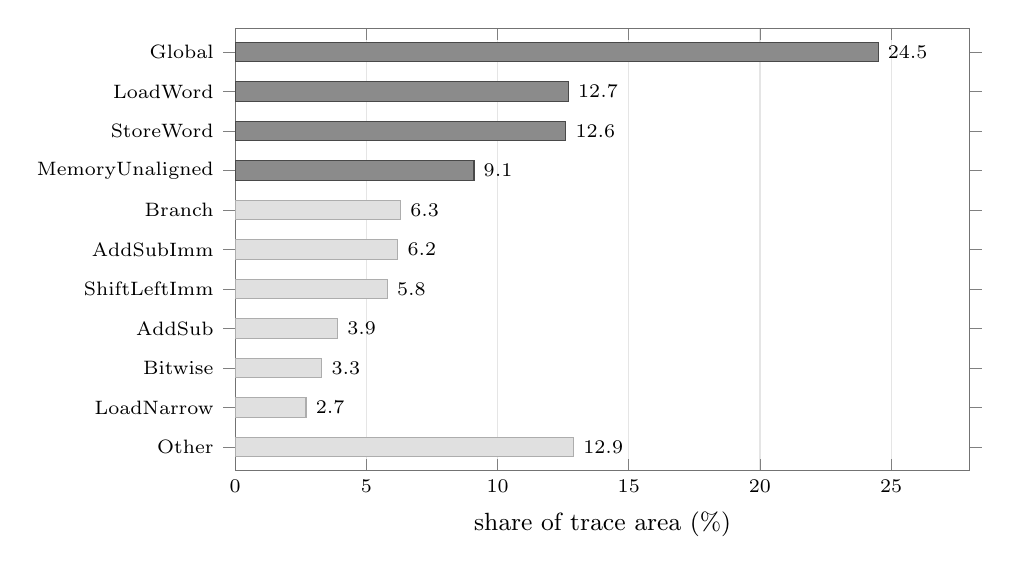
\begin{tikzpicture}
\begin{axis}[
  xbar, xmin=0, xmax=28, width=0.9\textwidth, height=7.2cm,
  bar width=7pt, xlabel={share of trace area (\%)},
  symbolic y coords={Other,LoadNarrow,Bitwise,AddSub,ShiftLeftImm,AddSubImm,Branch,MemoryUnaligned,StoreWord,LoadWord,Global},
  ytick={Other,LoadNarrow,Bitwise,AddSub,ShiftLeftImm,AddSubImm,Branch,MemoryUnaligned,StoreWord,LoadWord,Global},
  y dir=normal, nodes near coords, nodes near coords align={horizontal},
  every node near coord/.append style={font=\scriptsize},
  tick label style={font=\scriptsize}, label style={font=\small},
  xmajorgrids, grid style={black!10}, axis line style={black!55},
  enlarge y limits=0.06,
]
\addplot[fill=zirenslate!30, draw=zirenslate!80, bar shift=0pt] coordinates {
  (6.3,Branch) (6.2,AddSubImm) (5.8,ShiftLeftImm) (3.9,AddSub)
  (3.3,Bitwise) (2.7,LoadNarrow) (12.9,Other)};
\addplot[fill=zirenblue!65, draw=zirenblue!95!black, bar shift=0pt] coordinates {
  (24.5,Global) (12.7,LoadWord) (12.6,StoreWord) (9.1,MemoryUnaligned)
};
\end{axis}
\end{tikzpicture}
}\caption{Trace area by unit (19.6\,G cells); \texttt{Global} and the three largest memory-instruction units hold 59\%.}\label{fig:area}\end{subfigure}\hfill
\begin{subfigure}[t]{0.49\textwidth}\centering\resizebox{\linewidth}{!}{% GPU kernel time of the core lane by group (nsys, ten-shard sample).
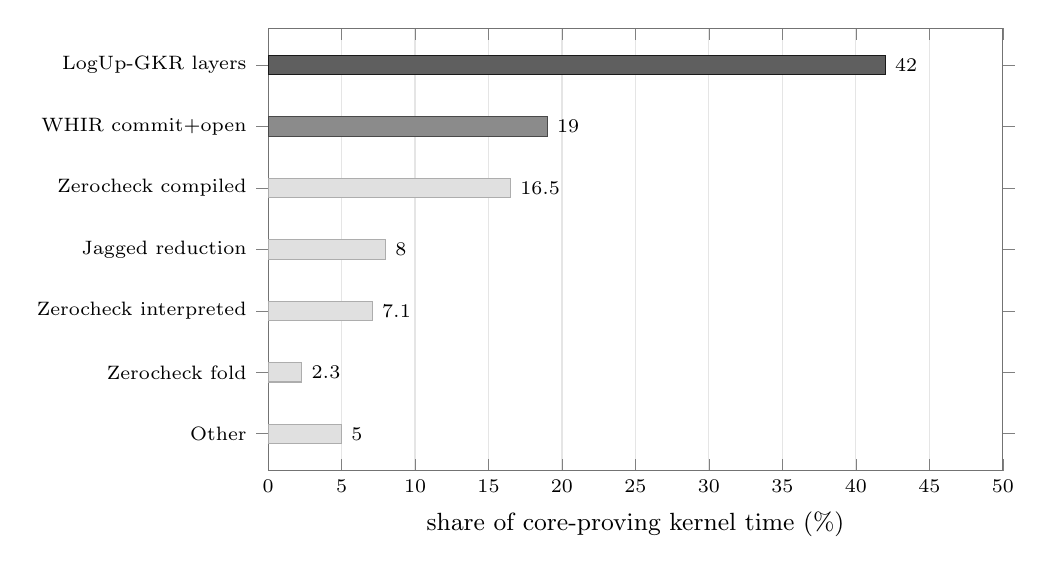
\begin{tikzpicture}
\begin{axis}[
  xbar, xmin=0, xmax=50, width=0.9\textwidth, height=7.2cm,
  bar width=7pt, xlabel={share of core-proving kernel time (\%)},
  symbolic y coords={Other,Zerocheck fold,Zerocheck interpreted,Jagged reduction,Zerocheck compiled,WHIR commit+open,LogUp-GKR layers},
  ytick={Other,Zerocheck fold,Zerocheck interpreted,Jagged reduction,Zerocheck compiled,WHIR commit+open,LogUp-GKR layers}, nodes near coords, nodes near coords align={horizontal},
  every node near coord/.append style={font=\scriptsize},
  tick label style={font=\scriptsize}, label style={font=\small},
  xmajorgrids, grid style={black!10}, axis line style={black!55},
  enlarge y limits=0.1,
]
\addplot[fill=zirenslate!30, draw=zirenslate!80, bar shift=0pt] coordinates {
  (16.5,Zerocheck compiled) (8,Jagged reduction) (7.1,Zerocheck interpreted) (2.3,Zerocheck fold) (5,Other)};
\addplot[fill=zirenorange!70, draw=zirenorange!95!black, bar shift=0pt] coordinates {
  (42,LogUp-GKR layers)};
\addplot[fill=zirenblue!65, draw=zirenblue!95!black, bar shift=0pt] coordinates {
  (19,WHIR commit+open)};
\end{axis}
\end{tikzpicture}
}\caption{\LogUp{} is the largest kernel group at 42\%, ahead of \WHIR{} commit and open at 19\% (nsys, ten-shard sample).}\label{fig:kernel}\end{subfigure}
\caption{The \texttt{Global} and three largest memory-instruction units hold 59\% of trace area, while \LogUp{} is the largest measured kernel group at 42\%. Both panels describe the evaluated pre-correction baseline before the changes of \S\ref{sec:perf-changes}.}
\label{fig:profile}
\end{figure}


\paragraph{What the soundness target costs.} The per-component target of
\S\ref{sec:iopp-soundness} is paid for in queries and in proof-of-work, and only
the first is visible in the proof. Measured on the workload block over four
cards of the eight-card host, with the other four carrying an unrelated proving
service throughout, each schedule reached from one binary through its
environment, and the arms interleaved: raising the query, \LogUp{} and batching grinds from
$16/16/8$ to $22/22/14$ bits left the block at $33.4$\,s against $33.9$\,s for
the former schedule, and buying the same bits with queries instead
($[133,95,91]$ at a 16-bit grind) cost $8.6$\%. Neither figure holds for a
prover whose proof-of-work search is not proportional to $2^{\text{bits}}$: the
same schedule took $166$\,s while the grinds ran on the host inside the
per-shard parallelism, $123$\,s of it the \LogUp{} grind alone. A grinding bit
is cheap for the honest prover only in the sense that the search is; it is not
free, and it buys a bit of soundness at the cost of a factor of two in that
search.

\subsection{What reducing area buys}
\label{sec:perf-changes}

The cost model of \S\ref{sec:perf-profile} says where to cut: area for the
commitment and the constraint argument, and \emph{(row, interaction)} pairs for
the bus argument. Four changes follow from it, three that remove columns or
interactions from the units the census names and one that raises the shard
size, and together they take the same block from 74.1 to 67.1\,s on one GPU,
a reduction of $9.4\%$. Two of them are worth naming because they are
mechanisms rather than tuning: replacing a boolean sign decomposition and its
witness columns in the cross-shard digest unit with three byte lookups, and
dropping byte checks on memory-instruction accesses that another unit already
enforces. Neither changes what any constraint reads, so the verifying keys and
the proofs are unchanged. Appendix~\ref{sec:app-levers} gives the four
measurements one at a time, and the two negative results that came with them:
a unit narrowed below measurement noise, and a shard size that did not fit in
device memory.

\subsection{Prover efficiency: memory traffic, and scaling across devices}
\label{sec:perf-after}

The profile identified the \LogUp{} circuit as the largest kernel consumer (42\%). A byte-level profile of its layers showed that the first layer paired adjacent fractions across the most-significant index bit, so that short units were carried through every layer of the tallest unit and the traffic summed over layers was 5.2$\times$ that of the first layer. Pairing on the least-significant bit instead lets each unit fold out after $\log_2$ of its own height. The change also frees enough memory for shards of twice the baseline size, which did not fit before it (\S\ref{sec:perf-changes}). The two are therefore enabled together, and the figure below reports the pair. We do not attribute the result to the layer order alone: separating them needs a 2-by-2 ablation over old/new pairing and baseline/doubled shard size, and the old-pairing/doubled-shard cell is the one that did not fit in memory, so that cell would have to be reported as a failure rather than a time. Until that experiment exists the result stands as one combined configuration change. With both, the same block proves in 48.7\,s on one GPU, against 67.8\,s for the revision without either at the largest shard size it could run ($-28\%$ for the pair; the 67.1\,s of Table~\ref{tab:levers} is a different revision), with the proof unchanged at 617\,618 bytes.

Table~\ref{tab:cards} reports the scaling of that configuration from one to four GPUs on a 420\,M-cycle block against the evaluated baseline of Table~\ref{tab:levers}. The throughput columns give proved guest cycles per second of wall-clock time. Figure~\ref{fig:scaling} plots throughput for three block sizes: 420, 530 and 912\,M cycles. The larger blocks take 84.3/44.7/26.5\,s and 124.3/65.0/38.0\,s on one, two and four GPUs. Throughput varies by less than 20\% across the three blocks. On the 420\,M-cycle block it scales by $1.9\times$ from one GPU to two and by $3.1\times$ to four; the two larger blocks reach $3.2\times$ and $3.3\times$ at four. The change helps least at four GPUs because it shortens core proving, whose share falls as the recursion tail and start-up ramp grow. The remaining gap to linear scaling comes from the serial recursion tail and from the interval before the emulator has produced enough shards to occupy every GPU.

\begin{figure}[t]
\centering
% Proved-execution throughput (MHz) against number of cards, three block sizes, after the lookup-layer change;
% the dashed line is the 288 M-cycle block on the historical pre-correction stack.
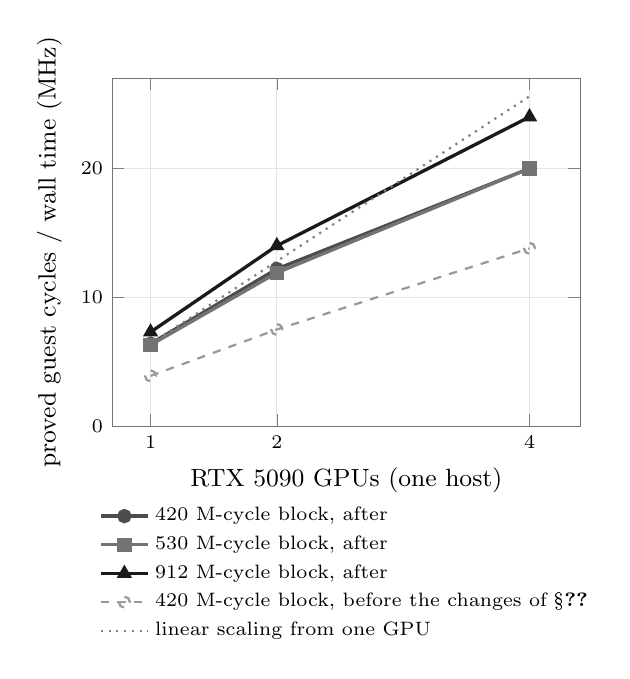
\begin{tikzpicture}
\begin{axis}[
  width=0.62\textwidth, height=6cm, xlabel={RTX 5090 GPUs (one host)}, ylabel={proved guest cycles / wall time (MHz)},
  xtick={1,2,4}, xmin=0.7, xmax=4.4, ymin=0, ymax=27, grid=major,
  grid style={black!10}, axis line style={black!55},
  legend style={font=\scriptsize, at={(0.5,-0.2)}, anchor=north, legend columns=1, cells={anchor=west}, draw=none},
  tick label style={font=\scriptsize}, label style={font=\small},
]
\addplot[color=zirenblue, mark=*, mark options={fill=zirenblue}, very thick] coordinates {(1,6.4) (2,12.2) (4,20.0)};
\addlegendentry{420 M-cycle block, after}
\addplot[color=zirenteal, mark=square*, mark options={fill=zirenteal}, very thick] coordinates {(1,6.3) (2,11.9) (4,20.0)};
\addlegendentry{530 M-cycle block, after}
\addplot[color=zirenorange, mark=triangle*, mark options={fill=zirenorange}, very thick] coordinates {(1,7.3) (2,14.0) (4,24.0)};
\addlegendentry{912 M-cycle block, after}
\addplot[color=zirenslate, mark=o, mark options={fill=white}, thick, dashed] coordinates {(1,3.9) (2,7.5) (4,13.8)};
\addlegendentry{420 M-cycle block, before the changes of \S\ref{sec:perf-after}}
\addplot[no marks, dotted, color=black!50, thick] coordinates {(1,6.4) (4,25.6)};
\addlegendentry{linear scaling from one GPU}
\end{axis}
\end{tikzpicture}

\caption{The pre-correction implementation reaches 3.1--3.3$\times$ one-GPU throughput on four GPUs across the three block sizes. The dotted line is ideal linear scaling; the baseline series is the evaluated zero-lookup-grinding configuration. None of the plotted throughput values measures the corrected release: every curve is the pre-correction Poseidon2 schedule, whose keys and proofs the correction invalidates (\S\ref{sec:perf-threats}), so the curves characterise scaling behaviour and not delivered performance.}
\label{fig:scaling}
\end{figure}

\begin{table}[t]
\centering
\caption{The lookup-layer and shard-size changes improve pre-correction throughput by $1.64\times$ on one GPU and $1.45\times$ on four GPUs for a 420\,M-cycle block. Values are warm wall-clock times for three consecutive proofs; the instrumented proof size was 617\,618 bytes.}
\label{tab:cards}
\begin{tabular}{lrrrrrr}
\toprule
 & \multicolumn{3}{c}{wall-clock (s)} & \multicolumn{3}{c}{throughput (MHz)} \\
\cmidrule(lr){2-4}\cmidrule(lr){5-7}
GPUs & 1 & 2 & 4 & 1 & 2 & 4 \\
\midrule
Before (evaluated baseline shards) & 108.0 & 56.0 & 30.5 & 3.9 & 7.5 & 13.8 \\
After (LSB pairing, doubled shards) & 65.9 & 34.3 & 21.0 & 6.4 & 12.2 & 20.0 \\
Speed-up & $1.64\times$ & $1.63\times$ & $1.45\times$ & & & \\
\bottomrule
\end{tabular}
\end{table}

\paragraph{Where the GPU work sits.} Three kinds of engineering carry the
figures above, and they are worth separating because they act on different
costs. \emph{Fused kernels} act on memory traffic: the jagged fold and the
round-polynomial evaluation it feeds are one kernel rather than two, so the
folded values stay in registers and shared memory instead of making a round
trip through device memory between them, and the same fusion is applied to the
layer transition and to the round over the mixed round-0 slab. \emph{A
cross-stage pipeline} acts on device idleness: the leaves and compose nodes of
the reduce tree are proved in single-device child processes while core shards
are still being proved (\texttt{core\_multi\_gpu::reduce\_overlap}), with one
tail worker for shrink and wrap, so the recursion tree is not a phase that
begins when core proving ends: on the measured block the root is delivered
before the last shard proof is. \emph{Occupancy tuning} acts on the kernels
themselves: the register budget is capped for the architecture of the card
measured here, which trades spills against resident warps.

Underneath all three, field arithmetic rests on the inline-PTX Montgomery
primitives of \texttt{sppark}~\citep{sppark}, which we use rather than wrote;
the \KB{} base and extension types are built on that layer, and no kernel of
ours emits assembly of its own. We separate this deliberately: the performance
reported here is a property of the whole stack, and the parts of the stack that
are other people's work are named as such.

\subsection{Answering the question of Section~\ref{sec:intro}}
\label{sec:perf-answer}

The opening question has three parts. \emph{Is the prover's cost attributable to identified choices?} The cost model of \S\ref{sec:perf-profile} names where the cost is, and the changes it suggested take the same block from 74.1 to 67.1\,s, $9.4\%$, with the per-change measurements in Appendix~\ref{sec:app-levers}. A further $28\%$ comes from the lookup-layer and shard-size pair of \S\ref{sec:perf-after}, which the section declines to separate for want of one cell of the ablation. Across those revisions the same block went from 74.1 to 48.7\,s and four GPUs reached 20\,MHz, but the corrected hash schedule remains unmeasured. Cross-system comparison is a different question, and this paper does not answer it. This paper reports what this prover costs and why, not how that compares: the figures other systems publish are self-reported, measured on different guests and mostly on clusters, and nothing here is a same-hardware baseline against any of them. \emph{What assumptions support soundness?} The proximity-test schedule uses the unique-decoding regime and a union bound, but the measured zero-lookup-grinding baseline does not inherit the checked-in report's 100-bit result. The random-oracle model, conditional extractor composition and unquantified structured-relation assumption for the cross-shard digest also remain. \emph{How much of the constraint system is verified?} The emulator is tested against an independent reference and formal model, \ndetproved{} of \ndettotal{} extracted determinism statements are closed, trace uniqueness has explicit premises, and the recursion machine is not extracted.

\subsection{Threats to validity}
\label{sec:perf-threats}

\emph{Internal validity.} All same-hardware comparisons are interleaved and repeated, and the measured spread is small relative to the reported effects; the one effect within the noise is reported as neutral. The host processor was shared with an unrelated process during the single-GPU measurements, so host-side interference was not controlled. \emph{Construct validity.} Every measurement used the pre-correction hash schedule whose partial-round count came from a higher S-box degree (\S\ref{sec:verification-findings}). Correcting it adds seven partial rounds to commitments, transcripts and recursion, invalidates the corresponding keys and proofs, and changes absolute performance by an unmeasured amount. The internal ablations remain evidence about the mechanisms only to the extent that the correction does not change their relative costs. Wall-clock time includes host verification, which a production deployment omits. Trace area is a cost model; the kernel profile is the direct measurement. \emph{External validity.} The primary workload is one Ethereum block. Other guests have different instruction mixes and per-unit area shares. No cross-system comparison is attempted, so nothing here establishes a ranking. No raw per-run timing bundle or exact 617\,618-byte proof is retained in the current artifact.

\section{Conclusion}
\label{sec:conclusion}

We have presented the second generation of \Ziren{} as an end-to-end verifiable-computation system for MIPS32 execution. Its executor feeds opcode-specific arithmetic tables; its instruction frame and shared bus arguments connect those tables to program, state and memory; its Jagged--\WHIR{} layer reduces columns of different heights to one batched opening; and its recursion and verifier turn shard proofs into one deployable artifact. Trace area, interaction count, proof size and accelerator throughput therefore describe one implemented CPU--GPU proof system, not a synthesisable processor.

We have also separated the evidence for this design into explicit layers. Conformance suites and an executable \Lean{} model test the emulator, while mechanically extracted statements expose determinism obligations in the constraint system. The current artifact closes \ndetproved{} of \ndettotal{} such statements and leaves recursion outside the extraction. At the proof-system layer, the unique-decoding accounting applies to the checked-in schedule, while end-to-end knowledge extraction remains conditional on the per-node and extractor-composition premises of Theorem~\ref{thm:composition}. The cross-shard digest remains a separate structured-relation assumption.

The performance study has identified trace area, lookup interactions, layer order and shard size as distinct cost levers. The largest item it leaves on the table is the cross-shard digest: every word touched in a shard costs two rows of that unit, one quarter of the block's area, and either a digest of the per-shard delta or a larger shard would reduce it, the latter bounded by the memory the lookup circuit's first layer needs. Its measurements characterise the pre-correction implementation and one block-proving workload; they do not establish corrected-release performance or a same-hardware ranking against other systems. The next release should unify one runtime configuration, soundness report, key set, serialised proof and benchmark bundle after the Poseidon2 correction. Completing the composition proof, quantifying the digest assumption and closing the remaining trace-uniqueness premises are the corresponding proof priorities.


\section*{Acknowledgements}

This system is built on work done by others, and two debts are large enough to
name here rather than only in citations. The Plonky3~\citep{plonky3} toolkit
supplies the field, the $\Poseidon{}$ permutation~\citep{poseidon2}, the
constraint interfaces and the transforms this implementation is written
against. SP1~\citep{sp1,sp1-hypercube} is the system this design learned the
most from: the decomposition into one chip per opcode with a shared lookup
argument, the elliptic-curve digest that carries interactions across shards,
the shadow read that makes register accesses cheaper than memory accesses, and
the shape of the recursion layer all follow it, and its just-in-time executor
is the model for ours. Where this paper departs from either, the section that
does so says why.

\appendix
\section{The just-in-time executor}
\label{sec:executor}

Section~\ref{sec:isa-emulator} states that the execution relation is realised
twice and says what connects the two realisations. This appendix gives the
mechanism of the second one, a just-in-time compiler for Linux x86-64 hosts,
which is what a production prover runs. Nothing in the protocol depends on it:
a platform without the compiler proves the same statements more slowly.

\subsection{Two implementations, three jobs}
\label{sec:exec-roles}

The interpreter is a single loop over \texttt{execute\_cycle}: fetch, dispatch
on the opcode, apply the state transition, append the events the trace
generator will consume. It implements every instruction, every syscall and
every error path, and it is the only implementation that emits the full event
record.

The compiler is used for the two jobs that dominate wall-clock time and need no
events. The first is \emph{whole-program execution}, when a caller wants only
the output stream and the exit status. The second, which the multi-GPU prover
depends on, is \emph{minimal-trace production}: the coordinating process runs
the guest to the end and emits, per shard, a chunk descriptor holding the
pre-access value of every memory word the shard reads, the register records at
its boundary, and the boundary itself. A worker then re-executes the shard from
that descriptor under the interpreter and emits the events locally. The
consequence is that no event record crosses a process boundary and the
coordinator holds one shard's state at a time, and also that the event-emitting
path stays the interpreter's: the compiler never has to reproduce an event
stream, only the state and the accounting a replay needs.

Availability is a build-time decision. The parent crate's build script emits
\texttt{cfg(zkm\_use\_native\_executor)} on Linux x86-64 without the profiling
feature; elsewhere the flag is absent and every entry point stays on the
interpreter, so a platform without the compiler is slower and not otherwise
different.

\subsection{Transpilation and the program cache}
\label{sec:exec-transpile}

Compilation is one-shot and per program, not per basic block discovered at run
time. The driver walks the program's instruction stream once, and for each
instruction records the native offset that the guest program counter maps to,
dispatches on the opcode to a lowering, and emits the epilogue that advances
the clock and the program counter. The result is a native code buffer, mapped
executable from an anonymous file, together with a jump table holding one
native address per guest program counter. Control transfers inside the compiled
program are table dispatches, so the compiled unit is the whole program and a
branch never leaves it.

Two properties of the lowering are worth stating because they are what make it
tractable. Delay slots are resolved statically: a branch or jump whose delay
slot holds another branch or jump, or which ends the program, is rejected at
compile time and the host falls back to the interpreter, so the only
instruction that has to read a delayed target is the one immediately after a
transfer. And an opcode the lowering does not model is a compile-time refusal
rather than a run-time surprise: the driver returns the offending opcode and
the caller falls back.

Compiled programs are cached process-wide. The key must be a hash of the entire
instruction stream: the base address, the instruction count and, for every
instruction, the opcode and all three operands with their immediate flags. A
cheaper fingerprint is unsound in a way that does not announce itself: two
guests that agree on a prefix and a suffix but differ in the middle collide,
and the second one silently executes the first one's code. \Ziren{} hashes the
whole stream for this reason, and a test asserts that changing any single
instruction changes the key.

\subsection{Machine state in host registers}
\label{sec:exec-state}

The guest's register file is held in host registers for the duration of a run.
There are 33 live guest registers (31 general-purpose plus \texttt{HI} and
\texttt{LO}) and 16 vector registers offering 32 half-slots, so exactly one
must live elsewhere: general registers 1 to 30 pack two per vector register
into the first fifteen, \texttt{HI} and \texttt{LO} take the halves of the
sixteenth, and the return-address register takes a general-purpose host
register of its own, because it is read and written by every call sequence and
a half-slot access costs an insert or extract. Register 0 is not stored at all.
The two registers that only \texttt{mmap}-style syscalls touch stay in the
context structure in memory.

Three quantities are pinned to host registers alongside the guest state: the
packed clock, the oracle tail pointer, and the remaining trace-area budget.
All three are written back to the context around any call into the host and on
exit, so the host never reads a stale copy.

Guest memory is a flat array with one sixteen-byte entry per guest word, a
value, the timestamp and shard of its last access, and padding that keeps the
index a shift of the address. The array is a shared mapping of an anonymous
file with reservation disabled, so it is sparse and only touched pages are ever
committed, and an unconstrained block is entered by mapping a private
copy-on-write view of the same file and left by unmapping it, so the rollback
that the paged executor performs with a per-address diff becomes one unmap. Two
alignments in that entry are load-bearing. Its first twelve bytes are exactly
the image of an oracle entry, so recording a pre-access value is one twelve-byte
copy; and its timestamp and shard fields are the little-endian image of the
packed clock register, so stamping an access is one eight-byte store.

\subsection{What the compiled code accounts for}
\label{sec:exec-accounting}

A compiled instruction is not just its state transition. To let a worker replay
a shard, and to close shards where the interpreter would, the emitted code also
performs the bookkeeping of Section~\ref{sec:isa}:

\begin{itemize}
  \item \textbf{Access stamps.} Every register the interpreter stamps is
  stamped here, with the same shard and the same sub-cycle position, at the
  highest position at which the instruction touches it.
  \item \textbf{The clock.} An instruction executes at $\mathsf{clk}$ and its
  accesses occupy $\mathsf{clk}+1,\dots,\mathsf{clk}+4$ by position, so the
  clock advances by five per instruction. The pinned register holds the shard
  and the clock as one word, which is what makes the memory stamp a single
  store.
  \item \textbf{The oracle.} A read or write of an address above the register
  window copies the entry as it stood before the access to the oracle tail,
  which is the descriptor the replaying worker will answer memory reads from.
  \item \textbf{Shard budgets.} The trace-area budget in its pinned register
  and the per-unit height budgets in the context are charged the exact amounts
  the interpreter's accumulator charges, supplied per instruction by the
  compiler. Exhaustion of any one of them is the condition under which the
  interpreter would fence, and the compiled function returns a shard-fence
  status so the host seals the chunk and re-enters.
\end{itemize}

Because the budgets are charged in native code and checked on every
instruction, the shard boundaries a compiled run produces are the boundaries an
interpreted run would produce, which is what allows the two to be compared
chunk by chunk.

\subsection{What the interpreter keeps}
\label{sec:exec-traps}

The compiler deliberately implements no error path and no syscall. Every
\texttt{SYSCALL}, every division by zero, every trap instruction, every
misaligned or out-of-range address, and every operand form the lowering does
not model is a \emph{trap site}: the emitted code stores the guest program
counter and jumps to a shared stub whose host handler synchronises the native
state into the interpreter, runs that one instruction there, synchronises back
and resumes the compiled code at the resulting program counter. The interpreter
therefore owns the precompiles, the unconstrained blocks and every failure, and
the compiler owns the arithmetic, memory and control flow that make up almost
every instruction of a real workload.

This split is what keeps the compiler small enough to argue about. It is also
why a syscall-dense guest sees less speedup than a compute-dense one: each trap
is a state synchronisation in both directions.

\subsection{Evidence that the two agree}
\label{sec:exec-equivalence}

Three checks connect the implementations, and none of them is a proof of
equivalence for every program.

The producer's output is compared against the interpreter's directly: tests
assert that the chunk descriptors a compiled run emits are byte-identical to
those of an interpreted run of the same program, which covers the state, the
oracle, the stamps and the shard boundaries in one comparison. The 770
specification vectors of Section~\ref{sec:verification} are executed on both
implementations and against an independent reference emulator. And continuous
integration compares digests of the emitted records across runs and across
implementations on the tested corpus, which is evidence of determinism and of
agreement there rather than everywhere.

Section~\ref{sec:perf-emu} measures what the compiler buys: on the reference
block it emulates the guest at roughly 130\,MHz against the
interpreter's 5--20\,MHz, depending on whether the interpreter
is recording events.

\subsection{The record pipeline under a host budget}
\label{sec:app-hostbudget}

Section~\ref{sec:perf-emu} states that on a host feeding several accelerators the executor, not the accelerator, is what binds, because each shard is re-emulated by the worker that proves it. The event stream written by one shard replay was approximately 1\,GB. Table~\ref{tab:host} lists the changes made under an explicit host budget. Each preserves the represented execution semantics: the trace columns every constraint reads are unchanged, so the verifying keys and the proofs are unchanged. The record layout itself does change; the table below removes fields and narrows record widths, so each change is witness-equivalent rather than byte-identical, and it is the event record, not the committed trace, whose bytes move.

\begin{table}[t]
\centering
\footnotesize
\setlength{\tabcolsep}{4pt}
\caption{Emulator and record pipeline under a host memory and processor budget. Sizes are per event or per shard of the block of \S\ref{sec:perf-setup}; times are host-side, single process, three repetitions.}
\label{tab:host}
\begin{tabular}{p{0.44\textwidth} r r p{0.27\textwidth}}
\toprule
Change & before & after & effect \\
\midrule
Per-cycle event: keep clock, \textsf{pc} pair and exit code only (no CPU table reads the rest) & 184\,B & 20\,B & event stream per shard 1{,}000\,MB $\to$ 462\,MB; replay 700\,ms $\to$ 435\,ms \\
Memory-instruction event: drop the three fields no column reads & 168\,B & 136\,B & every load/store event \\
Register-access record: carry only the witnessed values (no shard fields; one arm for read/write) & 48 / 24\,B & 20 / 16\,B & every instruction event \\
Memory oracle shipped to a worker: pre-access value, stamp and shard as one byte run & 24\,B, 25\,MB & 12\,B, 12\,MB & per access, per shard; serialise 6--7 $\to$ 1\,ms \\
Coordinator producer without checkpoints: no state clone or first-touch map per shard & 22.9\,s & 20.4\,s & per block; state $O(\text{shard})$ \\
Native (JIT) producer in the coordinator & 12.3\,s & 6.1\,s & per 420\,M-cycle block \\
Flat guest memory: one 16-byte entry per word in a sparse mapping; untouched pages cost nothing; unconstrained blocks are copy-on-write views & paged table & flat, sparse & no per-block memory diff \\
\bottomrule
\end{tabular}
\end{table}

Two rules follow. An event should carry exactly what a column witnesses: three of the seven rows remove fields that only a debug assertion or an unused code path had kept alive; on the shared register records alone this is 44 bytes for every instruction event, one write record and two read records. And the process that coordinates several GPUs should never hold the whole execution: the coordinator's resident state is one shard's oracle and the guest image, so the block size is not bounded by host memory; only the shard size is bounded, by the accelerator's memory (\S\ref{sec:perf-changes}). Both rules apply to any \zkVM{} whose prover is fed by a re-executing host.

\section{The guest instruction set}
\label{sec:app-isa}

This appendix lists the MIPS32 instructions a guest may execute, which is the
set the relation of \S\ref{sec:statement} quantifies over. It is also the
table from which the conformance corpus of \S\ref{sec:verification} is
generated: each row produces ten programs with pseudo-random operands,
boundary values and the delay-slot placements the instruction admits, giving
the 770 vectors compared against an independent emulator. The last column
names the chip that arithmetises the instruction, so the table fixes which
rows of Appendix~\ref{sec:app-chips} a program can occupy, and with it the
chip set that Section~\ref{sec:recursion} enumerates over.

Three conventions are worth noting. \texttt{HI} and \texttt{LO} occupy the
register file as registers 32 and 33, so the four moves between them and the
general registers are additions of an immediate zero rather than a chip of
their own. \texttt{SYNC}, \texttt{SYNCI} and \texttt{PREF} are accepted and
retire as no-ops, for which the same chip suffices. \texttt{SYSCALL} is absent
from the table because it is the boundary of the machine rather than a
computation within it; it is arithmetised by \texttt{SyscallInstrs} and its
interface is Section~\ref{sec:ipcore}.

\footnotesize
\begin{longtable}{@{}llll>{\raggedright\arraybackslash}p{0.27\textwidth}l@{}}
\caption{The 77 guest instructions, their primary encoding fields and the chip that proves each. \emph{Op} is bits 31--26 and \emph{func} bits 5--0; a dash marks a field the format does not use, and the immediate forms are distinguished from the register forms by \emph{Op} alone. Semantics are as transcribed from the architecture manual into the specification table that generates the conformance corpus.}\label{tab:isa}\\
\toprule
Mnemonic & Op & func & Family & Semantics & Chip \\
\midrule
\endfirsthead
\multicolumn{6}{@{}l}{\itshape Table~\ref{tab:isa}, continued from the previous page}\\
\toprule
Mnemonic & Op & func & Family & Semantics & Chip \\
\midrule
\endhead
\midrule
\multicolumn{6}{r@{}}{\itshape continued on the next page}\\
\endfoot
\bottomrule
\endlastfoot
\texttt{add} & \texttt{000000} & \texttt{100000} & Integer arithmetic & \texttt{rd = rs + rt} & \texttt{AddSub} \\
\texttt{addu} & \texttt{000000} & \texttt{100001} &  & \texttt{rd = rs + rt} & \texttt{AddSub} \\
\texttt{addi} & \texttt{001000} & \texttt{---} &  & \texttt{rt = rs + sext(imm)} & \texttt{AddSubImm} \\
\texttt{addiu} & \texttt{001001} & \texttt{---} &  & \texttt{rt = rs + sext(imm)} & \texttt{AddSubImm} \\
\texttt{sub} & \texttt{000000} & \texttt{100010} &  & \texttt{rd = rs - rt} & \texttt{AddSub} \\
\texttt{subu} & \texttt{000000} & \texttt{100011} &  & \texttt{rd = rs - rt} & \texttt{AddSub} \\
\texttt{mul} & \texttt{011100} & \texttt{000010} &  & \texttt{rd = rs * rt} & \texttt{Mul} \\
\texttt{mult} & \texttt{000000} & \texttt{011000} &  & \texttt{(hi, lo) = rs * rt} & \texttt{Mul} \\
\texttt{multu} & \texttt{000000} & \texttt{011001} &  & \texttt{(hi, lo) = rs * rt} & \texttt{Mul} \\
\texttt{div} & \texttt{000000} & \texttt{011010} &  & \texttt{(hi, lo) = (rs\%rt, rs/ rt), signed} & \texttt{DivRem} \\
\texttt{divu} & \texttt{000000} & \texttt{011011} &  & \texttt{(hi, lo) = (rs\%rt, rs/rt), unsigned} & \texttt{DivRem} \\
\texttt{madd} & \texttt{011100} & \texttt{000000} &  & \texttt{(hi, lo) = (hi,lo) + rs * rt (signed)} & \texttt{MiscInstrs} \\
\texttt{maddu} & \texttt{011100} & \texttt{000001} &  & \texttt{(hi, lo) = rs * rt + (hi,lo)} & \texttt{MiscInstrs} \\
\texttt{msub} & \texttt{011100} & \texttt{000100} &  & \texttt{(hi, lo) = (hi,lo) - rs * rt (signed)} & \texttt{MiscInstrs} \\
\texttt{msubu} & \texttt{011100} & \texttt{000101} &  & \texttt{(hi, lo) = (hi,lo) - rs * rt} & \texttt{MiscInstrs} \\
\texttt{clo} & \texttt{011100} & \texttt{100001} &  & \texttt{rd = count\_leading\_ones(rs)} & \texttt{CloClz} \\
\texttt{clz} & \texttt{011100} & \texttt{100000} &  & \texttt{rd = count\_leading\_zeros(rs)} & \texttt{CloClz} \\
\addlinespace
\texttt{slt} & \texttt{000000} & \texttt{101010} & Comparison and logic & \texttt{rd = rs < rt} & \texttt{Lt} \\
\texttt{sltu} & \texttt{000000} & \texttt{101011} &  & \texttt{rd = rs < rt} & \texttt{Lt} \\
\texttt{slti} & \texttt{001010} & \texttt{---} &  & \texttt{rt = rs < sext(imm)} & \texttt{LtImm} \\
\texttt{sltiu} & \texttt{001011} & \texttt{---} &  & \texttt{rt = rs < sext(imm)} & \texttt{LtImm} \\
\texttt{and} & \texttt{000000} & \texttt{100100} &  & \texttt{rd = rs \& rt} & \texttt{Bitwise} \\
\texttt{andi} & \texttt{001100} & \texttt{---} &  & \texttt{rt = rs \& zext(imm)} & \texttt{BitwiseImm} \\
\texttt{or} & \texttt{000000} & \texttt{100101} &  & \texttt{rd = rs | rt} & \texttt{Bitwise} \\
\texttt{ori} & \texttt{001101} & \texttt{---} &  & \texttt{rd = rs | zext(imm)} & \texttt{BitwiseImm} \\
\texttt{xor} & \texttt{000000} & \texttt{100110} &  & \texttt{rd = rs \textasciicircum{} rt} & \texttt{Bitwise} \\
\texttt{xori} & \texttt{001110} & \texttt{---} &  & \texttt{rd = rs \textasciicircum{} zext(imm)} & \texttt{BitwiseImm} \\
\texttt{nor} & \texttt{000000} & \texttt{100111} &  & \texttt{rd = !rs | rt} & \texttt{Bitwise} \\
\texttt{lui} & \texttt{001111} & \texttt{---} &  & \texttt{rt = imm<{}<16} & \texttt{AddSubImm} \\
\addlinespace
\texttt{sll} & \texttt{000000} & \texttt{000000} & Shifts and bit fields & \texttt{rd = rt<{}<sa} & \texttt{ShiftLeftImm} \\
\texttt{sllv} & \texttt{000000} & \texttt{000100} &  & \texttt{rd = rt <{}< rs[4:0]} & \texttt{ShiftLeft} \\
\texttt{srl} & \texttt{000000} & \texttt{000010} &  & \texttt{rd = rt >{}> sa} & \texttt{ShiftRightImm} \\
\texttt{srlv} & \texttt{000000} & \texttt{000110} &  & \texttt{rd = rt >{}> rs[4:0]} & \texttt{ShiftRight} \\
\texttt{sra} & \texttt{000000} & \texttt{000011} &  & \texttt{rd = rt >{}> sa} & \texttt{ShiftRightImm} \\
\texttt{srav} & \texttt{000000} & \texttt{000111} &  & \texttt{rd = rt >{}> rs[4:0]} & \texttt{ShiftRight} \\
\texttt{rotr} & \texttt{000000} & \texttt{000010} &  & \texttt{rd = rotate\_right(rt, sa)} & \texttt{ShiftRightImm} \\
\texttt{rotrv} & \texttt{000000} & \texttt{000110} &  & \texttt{rd = rotate\_right(rt, rs[4:0])} & \texttt{ShiftRight} \\
\texttt{ext} & \texttt{011111} & \texttt{000000} &  & \texttt{rt = rs[msbd+lsb..lsb]} & \texttt{MiscInstrs} \\
\texttt{ins} & \texttt{011111} & \texttt{000100} &  & \texttt{rt = rt[32:msb+1] || rs[msb+1-lsb : 0] || rt[lsb-1:0]} & \texttt{MiscInstrs} \\
\texttt{wsbh} & \texttt{011111} & \texttt{100000} &  & \texttt{rd = swaphalf(rt)} & \texttt{MovCond} \\
\texttt{seb} & \texttt{011111} & \texttt{100000} &  & \texttt{rd = signExtend(rt[7..0])} & \texttt{MiscInstrs} \\
\texttt{seh} & \texttt{011111} & \texttt{100000} &  & \texttt{rd = signExtend(rt[15..0])} & \texttt{MiscInstrs} \\
\addlinespace
\texttt{beq} & \texttt{000100} & \texttt{---} & Control transfer & \texttt{PC = PC + sext(offset<{}<2), if rs == rt} & \texttt{Branch} \\
\texttt{bne} & \texttt{000101} & \texttt{---} &  & \texttt{PC = PC + sext(offset<{}<2), if rs != rt} & \texttt{Branch} \\
\texttt{bgez} & \texttt{000001} & \texttt{---} &  & \texttt{PC = PC + sext(offset<{}<2), if rs >= 0} & \texttt{Branch} \\
\texttt{bgtz} & \texttt{000111} & \texttt{---} &  & \texttt{PC = PC + sext(offset<{}<2), if rs > 0} & \texttt{Branch} \\
\texttt{blez} & \texttt{000110} & \texttt{---} &  & \texttt{PC = PC + sext(offset<{}<2), if rs <= 0} & \texttt{Branch} \\
\texttt{bltz} & \texttt{000001} & \texttt{---} &  & \texttt{PC = PC + sext(offset<{}<2), if rs < 0} & \texttt{Branch} \\
\texttt{j} & \texttt{000010} & \texttt{---} &  & \texttt{PC = PC[GPRLEN-1..28] || instr\_index || 00} & \texttt{Jump} \\
\texttt{jal} & \texttt{000011} & \texttt{---} &  & \texttt{r31 = PC + 8, PC = PC[GPRLEN-1..28] || instr\_index || 00} & \texttt{Jump} \\
\texttt{jr} & \texttt{000000} & \texttt{001000} &  & \texttt{PC = rs} & \texttt{Jump} \\
\texttt{jalr} & \texttt{000000} & \texttt{001001} &  & \texttt{rd = PC + 8, PC = rs} & \texttt{Jump} \\
\texttt{bal} & \texttt{000001} & \texttt{---} &  & \texttt{RA = PC + 8, PC = PC + sign\_extend(offset || 00)} & \texttt{Jump} \\
\texttt{teq} & \texttt{000000} & \texttt{110100} &  & \texttt{trap, if rs == rt} & \texttt{MiscInstrs} \\
\addlinespace
\texttt{lb} & \texttt{100000} & \texttt{---} & Aligned memory & \texttt{rt = sext(mem\_byte(base + offset))} & \texttt{LoadNarrow} \\
\texttt{lbu} & \texttt{100100} & \texttt{---} &  & \texttt{rt = zext(mem\_byte(base + offset))} & \texttt{LoadNarrow} \\
\texttt{lh} & \texttt{100001} & \texttt{---} &  & \texttt{rt = sext(mem\_halfword(base + offset))} & \texttt{LoadNarrow} \\
\texttt{lhu} & \texttt{100101} & \texttt{---} &  & \texttt{rt = zext(mem\_halfword(base + offset))} & \texttt{LoadNarrow} \\
\texttt{lw} & \texttt{100011} & \texttt{---} &  & \texttt{rt = mem\_word(base + offset)} & \texttt{LoadWord} \\
\texttt{ll} & \texttt{110000} & \texttt{---} &  & \texttt{rt = mem\_word(base + offset)} & \texttt{LoadWord} \\
\texttt{sb} & \texttt{101000} & \texttt{---} &  & \texttt{mem\_byte(base + offset) = rt} & \texttt{StoreNarrow} \\
\texttt{sh} & \texttt{101001} & \texttt{---} &  & \texttt{mem\_halfword(base + offset) = rt} & \texttt{StoreNarrow} \\
\texttt{sw} & \texttt{101011} & \texttt{---} &  & \texttt{mem\_word(base + offset) = rt} & \texttt{StoreWord} \\
\texttt{sc} & \texttt{111000} & \texttt{---} &  & \texttt{mem\_word(base + offset) = rt, rt = 1, if atomic update, else rt = 0} & \texttt{StoreWord} \\
\addlinespace
\texttt{lwl} & \texttt{100010} & \texttt{---} & Unaligned memory & \texttt{rt = rt merge most significant part of mem(base+offset)} & \texttt{MemoryUnaligned} \\
\texttt{lwr} & \texttt{100110} & \texttt{---} &  & \texttt{rt = rt merge least significant part of mem(base+offset)} & \texttt{MemoryUnaligned} \\
\texttt{swl} & \texttt{101010} & \texttt{---} &  & \texttt{store most significant part of rt} & \texttt{MemoryUnaligned} \\
\texttt{swr} & \texttt{101110} & \texttt{---} &  & \texttt{store least significant part of rt} & \texttt{MemoryUnaligned} \\
\addlinespace
\texttt{mfhi} & \texttt{000000} & \texttt{010000} & Moves and no-ops & \texttt{rd = hi} & \texttt{AddSubImm} \\
\texttt{mflo} & \texttt{000000} & \texttt{010010} &  & \texttt{rd = lo} & \texttt{AddSubImm} \\
\texttt{mthi} & \texttt{000000} & \texttt{010001} &  & \texttt{hi = rs} & \texttt{AddSubImm} \\
\texttt{mtlo} & \texttt{000000} & \texttt{010011} &  & \texttt{lo = rs} & \texttt{AddSubImm} \\
\texttt{movn} & \texttt{000000} & \texttt{001011} &  & \texttt{rd = rs, if rt != 0} & \texttt{MovCond} \\
\texttt{movz} & \texttt{000000} & \texttt{001010} &  & \texttt{rd = rs, if rt == 0} & \texttt{MovCond} \\
\texttt{sync} & \texttt{000000} & \texttt{001111} &  & \texttt{sync (nop)} & \texttt{AddSubImm} \\
\texttt{synci} & \texttt{000001} & \texttt{---} &  & \texttt{sync (nop)} & \texttt{AddSubImm} \\
\texttt{pref} & \texttt{110011} & \texttt{---} &  & \texttt{prefetch(nop)} & \texttt{AddSubImm} \\
\addlinespace
\end{longtable}
\normalsize

\section{The unit set of the core machine}
\label{sec:app-units}

Section~\ref{sec:air} describes the arithmetisation as a set of units, a frame
and two shared arguments, without depending on which units exist. This appendix
is the catalogue of the units themselves. The widths matter only to the area
accounting: the protocol of Section~\ref{sec:argument} sees the whole shard as
one dense vector, so a unit may be added, widened or removed without changing
anything above the jagged reduction.

Every width in Table~\ref{tab:chips} was read from the machine at the commit
this paper describes (\S\ref{sec:perf-setup}) rather than from a census, and
the table lists all 62 units rather than the ones that dominate the area. That
pins it to one revision, which the evaluation's tables are not: the
measurements of \S\ref{sec:perf-changes} were taken on earlier revisions, so a
few units differ between them and this table. The \texttt{Global} unit is the
clearest case. It carries 65 columns here, against the 100 of the census in
\S\ref{sec:perf-profile} and the 58 that the change of \S\ref{sec:perf-changes}
reduced it to; work landed between that measurement and this commit. Where the
two disagree, the evaluation's numbers belong to the revision each table names
and this one belongs to the commit.

\begin{table}[t]
\centering
\small
\caption{The 62 units of the core machine with their main-trace widths (columns over $\F$), read from the machine of the release named in \S\ref{sec:perf-setup}; a second figure is a preprocessed width. The immediate (\texttt{Imm}) variants take the second operand from the instruction word. \texttt{MovCond} proves \texttt{movn}, \texttt{movz} and \texttt{wsbh}, and \texttt{SysLinux} the Linux-ABI syscalls of Section~\ref{sec:ipcore}; Appendix~\ref{sec:app-isa} gives the instruction-to-unit map.}
\label{tab:chips}
\begin{tabular}{p{0.2\textwidth} p{0.74\textwidth}}
\toprule
Family & Units (width) \\
\midrule
Integer ALU & \texttt{AddSub} (36), \texttt{AddSubImm} (33), \texttt{Bitwise} (37), \texttt{BitwiseImm} (33), \texttt{Mul} (74), \texttt{DivRem} (163), \texttt{Lt} (50), \texttt{LtImm} (47), \texttt{CloClz} (93) \\
Shifts & \texttt{ShiftLeft} (62), \texttt{ShiftLeftImm} (45), \texttt{ShiftRight} (89), \texttt{ShiftRightImm} (83) \\
Control flow & \texttt{Branch} (56), \texttt{Jump} (57) \\
Memory instructions & \texttt{LoadWord} (48), \texttt{LoadNarrow} (59), \texttt{StoreWord} (52), \texttt{StoreNarrow} (55), \texttt{MemoryUnaligned} (59) \\
Misc.\ / syscall & \texttt{MiscInstrs} (432), \texttt{MovCond} (49), \texttt{SyscallInstrs} (68), \texttt{SyscallCore} (11), \texttt{SyscallPrecompile} (11), \texttt{SysLinux} (100) \\
Memory argument & \texttt{MemoryLocal} (80), \texttt{MemoryBump} (12), \texttt{MemoryGlobalInit} (152), \texttt{MemoryGlobalFinalize} (152), \texttt{Global} (65) \\
Tables & \texttt{Program} (1, +14), \texttt{Byte} (10, +12), \texttt{Range} (1, +2) \\
Hash precompiles & \texttt{ShaExtend} (166) and control (4), \texttt{ShaCompress} (249) and control (69), \texttt{KeccakSponge} (2637) and control (1095), \texttt{Poseidon2Permute} (571) \\
Curve precompiles & add (1685) and double (1666) for \texttt{Secp256k1}, \texttt{Secp256r1} and \texttt{Bn254}, decompress (1040) for the first two; \texttt{Bls12381} add (2533), double (2506), decompress (1613); \texttt{Ed25519} add (1433), decompress (1166) \\
Field precompiles & \texttt{Bls12381Fp} (512), \texttt{Bls12381Fp2AddSub} (1014), \texttt{Bls12381Fp2Mul} (1773), \texttt{Bn254Fp} (344), \texttt{Bn254Fp2AddSub} (678), \texttt{Bn254Fp2Mul} (1181), \texttt{Uint256MulMod} (417), \texttt{U256XU2048Mul} (2627) \\
\bottomrule
\end{tabular}
\end{table}

\section{Per-change measurements}
\label{sec:app-levers}

Section~\ref{sec:perf-changes} reports one configuration end to end. This
appendix records the four changes one at a time, on the revision and workload
of \S\ref{sec:perf-setup}, together with the two that did not pay. Numbers of
this kind age with the revision they were taken on, and none of them is a
property of the protocol.

\begin{table}[t]
\centering
\caption{The four cumulative changes reduce the pre-correction single-GPU time from 74.1 to 67.1\,s on block 25\,907\,955. Values are medians of interleaved, host-verified runs; each row adds one change to the previous row.}
\label{tab:levers}
\begin{tabular}{lrrr}
\toprule
Configuration & shards & wall-clock (s) & vs.\ previous \\
\midrule
Evaluated baseline, no lookup grinding & 130 & 74.1 & \\
+ \texttt{Global} 100 $\to$ 58 columns (\S\ref{sec:air-global}) & 130 & 71.2 & $-3.9\%$ \\
+ memory-instruction accesses without byte checks (\S\ref{sec:air-memory}) & 130 & 70.2 & $-1.4\%$ \\
+ \texttt{ShiftLeftImm} 56 $\to$ 45 columns & 130 & 70.4 & neutral \\
+ shard size raised by a quarter & 114 & 67.1 & $-4.7\%$ \\
\midrule
All four vs.\ evaluated baseline & 114 & 67.1 & $-9.4\%$ \\
\bottomrule
\end{tabular}
\end{table}

The cost model of \S\ref{sec:perf-profile} suggested the changes in Table~\ref{tab:levers}. Replacing the 30-bit boolean sign decomposition, eight offset bits and seven chord-witness columns of the \texttt{Global} unit with three byte lookups removed 42 columns from 48\,M rows and 3.9\% of wall-clock time. The instrumented compressed-proof measurement remained 617\,618 bytes, while the core proofs, some $10^{8}$ bytes per block, shrank by 3.4\%. Removing redundant byte checks on memory-instruction accesses removed 5.7\% of the \LogUp{} pairs and 1.4\% of wall-clock time. This is less than the two-cells-per-pair model predicts because the lookup circuit's fold layers scale with padded heights rather than pair count. Reducing a 20\,M-row unit by 11 columns was below measurement noise; the 1.0\,s byte-check result was at its edge.

The largest single effect came from shard size. Raising it by a quarter removed 16 shards and saved 3.3\,s, approximately 0.2\,s per shard. Some shards close early on a unit's height budget, so the reduction is smaller than the cycle fence alone suggests. GPU memory limited larger shards at this revision: at 1.5 times the baseline size, the 4.5\,GiB first-layer \LogUp{} buffer caused repeated trim-and-retry and a 30\% slowdown; twice the baseline size did not fit in 32\,GB.


\section{System interfaces and integration}
\label{sec:app-ipcore}

This appendix collects the outward-facing description of the implemented system: what a deployer connects, what may be varied, how the prover and verifier are embedded, and which verification artifacts accompany a release. Section~\ref{sec:ipcore} fixes the corresponding system boundary.

\subsection{Ports}
\label{sec:ipcore-ports}

Table~\ref{tab:ports} lists the system interfaces. Five are fixed by the statement of Section~\ref{sec:statement}: a program image, an input stream and a hint stream go in, and a proof and its public values come out. The remaining three are supplied by a deployment: a verifying key derived once per program, a verifier that carries the key allowlist binding a recursion proof to the advertised machine, on an ordinary host or, after the wrap of Section~\ref{sec:recursion}, on chain, and an extension interface for guest accelerators.

\begin{table}[t]
\centering
\small
\caption{Interfaces of the proving and verification system. ``Setup'' interfaces are used once per program; ``run'' interfaces once per execution.}
\label{tab:ports}
\begin{tabular}{>{\raggedright\arraybackslash}p{0.18\textwidth} >{\raggedright\arraybackslash}p{0.10\textwidth} >{\raggedright\arraybackslash}p{0.58\textwidth}}
\toprule
Port & When & Contents \\
\midrule
Program image & setup & a little-endian MIPS32 ELF produced by the guest toolchain (GCC, LLVM or the Rust target); its text and initial data become the program ROM and the initial memory \\
Verifying key & setup & the Merkle commitment to the program ROM and the preprocessed tables (Section~\ref{sec:air}); 304 bytes, derived deterministically from the image; identifies the program in the statement \\
Input stream & run & the bytes the guest reads as its standard input; a witness \\
Hint stream & run & host-supplied data the guest reads through the hint syscall (for example the block witness); a witness, written into untouched memory and thereby bound by the memory argument \\
Public values & out & the digest of the committed output, the exit code, the entry and exit machine state, the address cursors of the global memory tables and the septic digest (Section~\ref{sec:isa}) \\
Compressed proof & out & the root of the recursion tree, 603\,KiB for the block of Section~\ref{sec:performance}; optionally wrapped to a Groth16 proof over BN254 for on-chain verification (Section~\ref{sec:recursion}) \\
Verifier & deliverable & a verifier that checks a compressed proof on an ordinary host, small enough to embed in the consuming application; it carries the recursion-key allowlist \\
Accelerator interface & extension & a syscall number, an emulator hook that reads and writes guest memory at the invoking cycle, and a chip that receives the syscall tuple (arguments as 16-bit half-words plus the Linux flag) on the syscall bus and performs its memory accesses on the memory bus (Section~\ref{sec:isa}) \\
\bottomrule
\end{tabular}
\end{table}

\subsection{Configuration space}
\label{sec:ipcore-config}

The proving system is parameterised, and Section~\ref{sec:performance} walks through part of its configuration space. Parameters include shard size, commitment stacking height, the \WHIR{} schedule, lookup-challenge grinding, recursion arity and guest-accelerator set. The \WHIR{} schedule fixes committed rounds, folding factors, code rates, queries, out-of-domain samples and query grinding, thereby setting proof size and soundness accounting (Section~\ref{sec:iopp}). The guest-accelerator set determines precompile chips and their verifying keys. Release values belong in one configuration file. A constraint-system parameter changes the affected chip keys and the recursion-key allowlist; a schedule-only parameter changes recursion-program keys but not chip keys.

\subsection{Integration paths}
\label{sec:ipcore-integration}

The integrations below share the same interfaces. The common shape is a guest that hashes: it recomputes a Merkle root over data the verifier does not hold, checks an inclusion or update proof, verifies a chain of signatures or certificates, or attests a firmware image or a log. The guest is compiled by an ordinary MIPS toolchain, calls the hash accelerators of Section~\ref{sec:isa} where the volume justifies it, and the verifier checks one proof whose cost does not grow with the amount hashed.

Three specialisations are worth naming. In \emph{block proving}, the deployed case, a coordinating process cuts a native execution into shards and ships a descriptor per shard to one worker process per GPU, which re-execute and prove their shards and the recursion nodes above them; \S\ref{sec:perf-host} describes the host budget this pipeline was engineered against. In \emph{hybrid fault and validity proving}, one program image is adjudicated by a fault proof and certified by a validity proof without a second toolchain, because \Ziren{} executes the instruction set Cannon and Kona already execute~\citep{cannon,kona}. In \emph{embedded and IoT workloads}, a program compiled by a device's own MIPS toolchain is executed by a remote prover and a gateway checks the proof, so the statement is the execution of the device's software rather than a property of the device (\S\ref{sec:related}). We report no measurement of the wrapped on-chain path, and Section~\ref{sec:verification-findings} records two omissions found in the terminal circuits it depends on.

\subsection{Verification artifacts}
\label{sec:ipcore-collateral}

A release includes the verification artifacts of Section~\ref{sec:verification}: the specification-derived conformance suite and Cannon reference results; the executable \Lean{} ISA model and its checks against the emulator; one extracted determinism statement per chip and opcode selector, together with the tactic and list of open statements; the soundness configuration and generated accounting report; and the defects register of Table~\ref{tab:defects}. The checked-in accounting configuration uses 16 bits of lookup grinding and therefore differs from the measured zero-grinding baseline. A deployer must verify that the toolchain, runtime configuration, verifier binary, key allowlist and accounting report identify the same release. The current artifacts test ISA correspondence and close \ndetproved{} of \ndettotal{} determinism statements; they do not replace the open chip proofs, the trace-exhaustiveness premise or the unverified recursion machine.


\section{Defects surfaced by the verification flow}
\label{sec:app-defects}

\begin{table}[t]
\centering
\small
\caption{Defects surfaced by the verification flow. ``Theorem'' means the extracted determinism theorem of the chip; ``proving'' means an end-to-end proof of a real block or of the test programs; ``review'' means a line-by-line comparison of this design against the RISC-V system it descends from, reading both implementations side by side.}
\label{tab:defects}
\begin{tabular}{>{\raggedright\arraybackslash}p{0.17\textwidth} >{\raggedright\arraybackslash}p{0.34\textwidth} >{\raggedright\arraybackslash}p{0.09\textwidth} >{\raggedright\arraybackslash}p{0.24\textwidth}}
\toprule
Component & Defect & Found by & Resolution \\
\midrule
Syscall chip & argument half-words not determined by the reduced argument ($2^{32} > p$) & theorem & half-words carried on the syscall bus; theorem closes \\
Syscall chip & result columns gated by a selector that no input pins & theorem & selector carried on the syscall bus; theorem closes \\
Extractor & shard and clock fields of syscall interactions dropped, leaving outputs without inputs & theorem & extractor fixed \\
Shape configuration & range table absent from the preprocessed heights; every shape-fixed proving test failed & proving & height registered \\
Standalone verifier & recursion-key Merkle root computed from the bare key list while the prover pads to the tree height & proving & verifier pads the leaves \\
Proving service & configured to skip the in-circuit key check, producing proofs the standalone verifier rejects & proving & service configuration \\
Recursion, terminal stages & the completeness flag gates every completeness predicate, including the one forcing the cross-shard sum to zero, but neither terminal circuit pinned it; an execution-prefix proof could therefore be wrapped & review & both terminal circuits assert it; the deferred program can no longer emit it set \\
Core, cross-shard state & the entry and exit state of a delayed-branch machine is the pair (pc, next pc), but only the first component was pinned across shards: the second was unreferenced in the recursion circuit, the prover and the verifier, so a prover could choose each shard's continuation address & review & both components asserted in the leaf circuit and the host verifier; a forgery test rejects a shifted pair \\
Wrap circuit, opening & the recursive \BaseFold{} verifier asserted only the query chain, with no sumcheck message or terminal identity, and read its query count as the smaller of the schedule's and the list the prover supplied & review & both identities asserted in-circuit and the count taken from the schedule, a short list rejected (\S\ref{sec:iopp-outer}) \\
Wrap circuit & the recursion-key allowlist root was not a public input, so no external verifier could require the published one & review & exposed as a public input and checked by the standalone and on-chain verifiers \\
Hash parameters & partial-round count taken from the tabulation for S-box degree seven rather than three, giving less algebraic-attack margin than intended & review & schedule corrected; the measurements of Section~\ref{sec:performance} predate the change \\
\bottomrule
\end{tabular}
\end{table}


% Clear the appendix's pending floats before the references, so a large
% appendix table cannot be deferred past the bibliography heading and then
% interrupt the entry list.
\clearpage

\bibliographystyle{alpha}
\bibliography{references}

\end{document}
